\documentclass[twoside]{article}

%\usepackage[b6j,left=1cm,right=1cm,top=1cm,bottom=1cm]{geometry}
\usepackage[b5j, inner=2cm,outer=3cm,top=2cm,bottom=3cm, headsep=1.5\baselineskip, includehead]{geometry}

\usepackage{fancyhdr}
\fancyhf{}
\fancyhead[EL]{\textbf\thepage \qquad \footnotesize\leftmark}
\fancyhead[OR]{{\footnotesize MAS312 2023 Fall: Lecture note}\qquad \textbf\thepage}
\renewcommand\headrulewidth{0pt}
\pagestyle{fancy}

\let\oldIm=\Im
\let\Im=\relax

\usepackage{mathtools}
\DeclareMathOperator\Aut{Aut}
\DeclareMathOperator\Char{char}
\DeclareMathOperator\End{End}
\DeclareMathOperator\Gal{Gal}
\DeclareMathOperator\id{id}
\DeclareMathOperator\Im{Im}
\DeclareMathOperator*\lcm{lcm}
\DeclareMathOperator\ord{ord}
\DeclareMathOperator\sgn{sgn}

\renewcommand\rmdefault{minntx}
\usepackage[cochineal]{newtx}
%\usepackage{amssymb}
\newcommand\N{\mathbb N}
\newcommand\Z{\mathbb Z}
\newcommand\Q{\mathbb Q}
\newcommand\R{\mathbb R}
\newcommand\C{\mathbb C}
\newcommand\F{\mathbb F}

\usepackage[dvipsnames]{xcolor}
\colorlet{myblue}{ProcessBlue} % major helper lines
\colorlet{myyellow}{Dandelion} % minor helper lines
\colorlet{myred}{RubineRed} % color for the result

\let\openbox=\relax
\usepackage{amsthm}
%\newtheorem{theorem}{Theorem}[section]
%\newtheorem{proposition}[theorem]{Proposition}
%\newtheorem{lemma}[theorem]{Lemma}
%\newtheorem{corollary}[theorem]{Corollary}
%\theoremstyle{definition}
%\newtheorem*{definition}{Definition}
\theoremstyle{remark}
\newtheorem*{remark}{{Remark}}
\newtheorem*{remarks}{{Remarks}}
\newtheorem{note}{Note}
\newtheorem*{recall}{Recall}
%\newtheorem*{example}{Example}
%\newtheorem*{examples}{Examples}
\newtheorem*{property}{Property}
\newtheorem*{properties}{Properties}

\usepackage{subcaption}

\renewcommand*{\qedsymbol}{\(\blacksquare\)}

\usepackage{tcolorbox}
\tcbuselibrary{breakable}
\tcbset{boxsep=0pt, left=10pt, right=7.5pt, top=7.5pt, bottom=7.5pt, beforeafter skip balanced=10pt plus 5pt, parbox=false}

\usepackage{tikz}
\usetikzlibrary{angles}
\usetikzlibrary{calc}
\usetikzlibrary{intersections}

\usepackage{tikz-cd}

\usepackage{enumitem}
\setlist{listparindent=\parindent}

\usepackage{makeidx}
\makeindex

\usepackage[colorlinks=true, linkcolor=black]{hyperref}

\newtcolorbox{definition}[1][\relax]{colframe=black, colback=black!3, toprule=0pt, bottomrule=0pt, leftrule=2pt, rightrule=0pt, arc=0pt, before upper = \textbf{Definition\def\temp{#1}\def\ttemp{\relax}\ifx\temp\ttemp\else\ (\temp)\fi. }}

\newcounter{theorem}
\counterwithin{theorem}{section}
\newtcolorbox[use counter* = theorem]{theorem}[1][\relax]{colframe=cyan, colback=cyan!5, fontupper=\slshape, toprule=0pt, bottomrule=0pt, leftrule=2pt, rightrule=0pt, arc=0pt, before upper = \textbf{\upshape Theorem \thetheorem\def\temp{#1}\def\ttemp{\relax}\ifx\temp\ttemp\else\ (\temp)\fi. }}
\newtcolorbox[use counter* = theorem]{proposition}[1][\relax]{colframe=cyan, colback=cyan!5, fontupper=\slshape, toprule=0pt, bottomrule=0pt, leftrule=2pt, rightrule=0pt, arc=0pt, before upper = \textbf{\upshape Proposition \thetheorem\def\temp{#1}\def\ttemp{\relax}\ifx\temp\ttemp\else\ (\temp)\fi. }}
\newtcolorbox[use counter* = theorem]{corollary}[1][\relax]{colframe=cyan, colback=cyan!5, fontupper=\slshape, toprule=0pt, bottomrule=0pt, leftrule=2pt, rightrule=0pt, arc=0pt, before upper = \textbf{\upshape Corollary \thetheorem\def\temp{#1}\def\ttemp{\relax}\ifx\temp\ttemp\else\ (\temp)\fi. }}
\newtcolorbox[use counter* = theorem]{lemma}[1][\relax]{colframe=cyan, colback=cyan!5, fontupper=\slshape, toprule=0pt, bottomrule=0pt, leftrule=2pt, rightrule=0pt, arc=0pt, before upper = \textbf{\upshape Lemma \thetheorem\def\temp{#1}\def\ttemp{\relax}\ifx\temp\ttemp\else\ (\temp)\fi. }}
\newtcolorbox{example}{colframe=violet, colback=violet!4, toprule=0pt, bottomrule=0pt, leftrule=2pt, rightrule=0pt, arc=0pt, before upper = \textbf{Example. }\par\small\let\small=\footnotesize, breakable}
\newtcolorbox{examples}{colframe=violet, colback=violet!4, toprule=0pt, bottomrule=0pt, leftrule=2pt, rightrule=0pt, arc=0pt, before upper = \textbf{Examples. }\small\let\small=\footnotesize, breakable}

\counterwithin{figure}{section}

\flushbottom

\newcommand*\term[1]{\textbf{\textit{\mathversion{bold}#1}}}

%\newcommand*\newclass[1]{\noindent\textcolor{gray}{\hrulefill\quad \textsf{#1}\quad\hrulefill}\par\vskip2ex\nopagebreak}
%\newcommand*\newclass[1]{\par\marginpar{\footnotesize\textsf{#1}}\ignorespaces}
\newcommand*\newclass[1]{\par\vbox to 0pt{\hbox{\tiny\sffamily\color{gray}#1}} \par\ignorespaces}

\title{\sffamily\bfseries MAS312 Modern Algebra II}
\author{\sffamily Instructor: Sanghoon Baek}
\date{\sffamily 2023 Fall}

\begin{document}
\maketitle
\thispagestyle{empty}

This document is the lecture note of Modern Algebra II course in KAIST, held in Fall, 2023. The instructor for this course is Sanghoon Baek. This note is written by Woohyun Kang. It does not contain materials from practice classes.

\tableofcontents

\clearpage


\part{Ring Theory}

\section{Rings}

\newclass{28-08-23}
\noindent \textit{Recall}.

\begin{definition} \index{ring}
  A \term{ring} \(R\) is a set with \(a+b\) and \(ab \in R\) for all \(a,b \in R\) satisfying
  \begin{enumerate}[label=(\arabic*), nosep]
    \item \((R,+)\) is an abelian group.
    \item \((ab)c = a(bc)\) for all \(a,b,c \in R\).
    \item \((a+b)c = ac + bc\), \(a(b+c) = ab + ac\) for all \(a,b,c \in R\).
    \item \(1 \in R\) with \(a1 = 1a = a\) for all \(a \in R\) exists.
  \end{enumerate}
\end{definition}

\begin{definition} \index{commutative ring}\index{division ring}\index{field}\index{zero divisor}
  \begin{enumerate}[label=\arabic*.]
    \item \term{Commutative ring}: \(ab = ba\) for all \(a,b \in R\).
    \item \term{Division ring}: \(1 \neq 0\) (\(\leftrightarrow\) nonzero ring), \(R^\times = R \setminus \{0\}\). \\
    \(R^\times = \{a \in R \mid \text{\(a\) has an inverse}\}\), called group of units.
    \item \term{Field}: commutative division ring.
    \item An element \(a\) of a ring \(R\) is called a \term{left zero divisor} (resp.\ \term{right zero divisor}) if there exists a nonzero element \(b \in R\) such that \(ab=0\)(resp.\ \(ba=0\)). \\
    If \(R\) is a commutative ring, left zero divisors \(\equiv\) right zero divisors.
    \item \term{(Integral) domain}: commutative and \(0\) is the only zero divisor.
  \end{enumerate}
\end{definition}

\[ \left[ \parbox{1.9cm}{\centering Commutative rings} \right] \supset \left[ \parbox{1.3cm}{\centering Integral domains} \right] \supset \left[ \parbox{1.8cm}{\centering Unique factorization domains} \right] \supset \left[ \parbox{2cm}{\centering Principal ideal domains} \right] \supset \left[ \parbox{1.4cm}{\centering Euclidean domains} \right] \supset \text{[Fields]} \]
\[ \text{[Integral domains]} \supset \text{[Integrally closed domains]} \supset \text{[Unique factorization domains]} \]

\begin{definition}\index{principal ideal ring}\index{principal ideal domain}\index{P.I.D.}%
  A commutative ring \(R\) is called a \term{principal ideal ring (P.I.R.)} if every ideal of \(R\) is principal (i.e., every ideal of \(R\) is generated by a single element), or equivalently, if \(I\) is an ideal of \(R\), then \(I = Ra (= \{ra \mid r \in R\})\) for some \(a \in R\). We use the notations \(Ra = \langle a \rangle = (a)\). \par
  An integral principal ideal ring (= P.I.R. which is an integral domain) is called a \term{principal ideal domain (P.I.D.)}.
\end{definition}

\begin{examples}
  \begin{enumerate}[label=\arabic*.]
    \item Fields, \(\Z\): P.I.D.s \\
    For a field \(F\), \(\{0\} = (0)\) and \(F = (1)\) are all ideals of \(F\). \\
    Every ideal of \(\Z\) is of the form \(n\Z = (n)\) for some \(n \in \Z\).
    \item \(\Z[x]\) is not a P.I.D. as \((2,x) = 2\Z[x] + x\Z[x]\) is not a principal. \\
    (If \((2,x) = (f)\) for some \(f \in \Z[x]\), then \(\deg f = 0\), but \(x \notin (f)\).)
    \item \(\R \times \Z\) is a principal ideal ring but not principal ideal domain. \\
    Ideals of \(\R\) are \(\{0\}\) and \(\R\), and ideals of \(\Z\) are of the form \(n\Z\). Thus, an ideal of \(\R \times \Z\) is of the form \(\{0\} \times n\Z = \langle(0,n)\rangle\) or \(\R \times n\Z = \langle(1,n)\rangle\). \\
    \((0,1) \cdot (1,0) = (0,0)\) are zero divisors.
  \end{enumerate}
\end{examples}

\begin{proposition}
  Every nonzero prime ideal in a P.I.D. is maximal.
\end{proposition}

\begin{proof}
  Let \(P = (a)\) be a prime ideal for some \(a \in R\), where \(R\) is a P.I.D.\@ By Zorn's lemma, \(P \subset I = (b)\) for some maximal ideal \(I\) of \(R\) and some \(b \in R\). Then, \(a = br\) for some \(r \in R\). As \(P\) is prime, \(b \in P\) or \(r \in P\). If \(r \in P\), then \(r = as = brs\) for some \(s \in R\), \(1 = bs\). Hence, \(I = R\), a contradiction. Therefore, we have \(b \in P\), so \(P = I\).
\end{proof}

\begin{definition}[Euclidean Domain] \index{Euclidean ring}\index{Euclidean domain}\index{E.D.}
  A commutative ring \(R\) is called a \term{Euclidean ring} if there exists a map \(\varphi: R \setminus \{0\} \to \N \cup \{0\}\) such that for any \(a,b \neq 0 \in R\), there exists \(q,r \in R\) such that \(a = bq+r\) with either \(r=0\) or \(\varphi(r) < \varphi(b)\). \par
  A Euclidean ring which is an integral domain is called a \term{Euclidean domain (E.D.)}.
\end{definition}

\begin{examples}
  \begin{enumerate}[label=\arabic*.]
    \item Every field is a Euclidean domain with any \(\varphi\) because \(a = b(b^{-1}a) + 0\) if \(b \neq 0\).
    \item \(R = \Z\), \(\varphi(n) = |n|\) is a E.D.\@
    \item \(R = F[x]\) with a field \(F\), \(\varphi(f) = \deg f\) is a Euclidean domain.
    \item \(R = \Z[x]\) is not a E.D. as \(R\) is not a P.I.D.\@ \\
    (E.D. \(\Rightarrow\) P.I.D.)
    \item \(R = \Z[i] = \{a + bi \mid a, b \in \Z\}\) with \(\varphi(x) = |x|^2\) (i.e., if \(x = a+bi\), then \(\varphi(x) = (a+bi)(a-bi) = a^2+b^2\)) is a E.D.\@ \par
    Let \(x,y \neq 0 \in R\). Then
    \[ \frac xy \in \Q[i] = \{u + iv \mid u,v \in \Q\}. \]
    Write \(x/y = u + iv\). If \(u,v \in \Z\), then \(x = y(u+iv) + 0\). Otherwise, find \(a\) and \(b\) in \(\Z\) such that \(|u-a| \leq 1/2\) and \(|v-b| \leq 1/2\). Set \(q = a+bi\). Then \(x/y - q = (u-a) + i(v-b)\) and
    \[ \left| \frac xy - q \right|^2 = (u-a)^2 + (v-b)^2 \leq \frac14 + \frac14 < 1 \]
    Then \(|x-qy|^2 < |y|^2\). Set \(r = x-qy\). Then \(\varphi(r) < \varphi(y)\).
  \end{enumerate}
\end{examples}

\begin{theorem}
  Every Euclidean domain is a principal ideal domain.
\end{theorem}

\begin{proof}
  Let \(I \neq 0\) be an ideal of a E.D. \(R\) with \(\varphi\). Consider \(S = \{\varphi(a) \mid a \neq 0 \in I\}\). Choose \(a \in I\) such that \(\varphi(a)\) is the smallest integer in \(S\). Then \(I = Ra\). \par
  (Let \(b \in I\). Then, \(b = qa + r\) for some \(q,r \in R\). If \(r \neq 0\), then \(\varphi(r) < \varphi(a)\) and \(r = b-qa \in I\), a contradiction. Hence, \(r=0\), \(b = qa \in Ra\).)
\end{proof}

\begin{remark}
  The converse statement may not hold in general:
  \[ \Z[\alpha] = \{a + b\alpha \mid a,b \in \Z\}, \qquad \alpha = \frac{1+\sqrt{-19}}2 \]
  is a P.I.D. but not a E.D.
\end{remark}

\newclass{30-08-23}

\begin{definition} \index{divisible}\index{associate}
  Let \(R\) be a commutative ring and let \(a, a', b \in R\) with \(b \neq 0\).
  \begin{enumerate}[label=\arabic*.]
    \item We say that \(a\) is \term{divisible} by \(b\) if \(a=bc\) for some \(c \in R\). \\
    (We use the notation \(b \mid a\).)
    \item Two elements \(a\) and \(a'\) are called \term{associate} if \(a \mid a'\) and \(a' \mid a\). \\
    (We use the notation \(a \sim a'\).)
  \end{enumerate}
\end{definition}

\begin{remarks}\phantom{}
  \begin{enumerate}[label=\arabic*.]
    \item \(b \mid a \iff aR \subset bR\) and \(a \sim b \iff aR = bR\).
    \item Let \(u \in R^\times\). Then, 
    \begin{itemize}[label=\textbullet, nosep]
      \item \(u \mid a\) for all \(a \in R\) (as \(a = u \cdot (u^{-1}a)\)).
      \item \(u \sim 1\) (as \(uR = R = 1 \cdot R\)).
      \item \(a \sim au\) (as \(auR = aR\)).
    \end{itemize}
    \item If \(R\) is a domain, then \(a \sim b \leftrightarrow a = bu\) for some \(u \in R^\times\): \\
    \(\leftarrow\) \(aR = buR = bR\) \\
    \(\rightarrow\) \(a \in aR = bR\). Then \(a = bc\) for some \(c \in R\). As \(b \in aR = bR\), \(b = ad\) for some \(d \in R\). Hence, \(a = bc = ad\), thus \(1 = dc\), i.e., \(c \in R^\times\).
  \end{enumerate}
\end{remarks}

\begin{definition} \index{irreducible}\index{prime}
  Let \(R\) be a domain.
  \begin{enumerate}[label=\arabic*.]
    \item An element \(c \in R\) is called \term{irreducible} if
    \begin{enumerate}[label=(\arabic*), nosep]
      \item \(c \neq 0\), \(c \notin R^\times\)
      \item \(c = ab\) for some \(a,b \in R\) implies \(a \in R^\times\) or \(b \in R^\times\).
    \end{enumerate}
    \item An element \(p \in R\) is \term{prime} if
    \begin{enumerate}[label=(\arabic*), nosep]
      \item \(p \neq 0\), \(p \notin R^\times\)
      \item \(p \mid ab\) for some \(a,b \in R\) implies \(p \mid a\) or \(p \mid b\).
    \end{enumerate}
  \end{enumerate}
\end{definition}

\begin{examples}\phantom{}
  \begin{enumerate}[label=\arabic*.]
    \item \(R = \Z\), \(R^\times = \{\pm 1\}\) \\
    Let \(a \in R\). Then, \(a\) is irreducible \(\iff\) \(a\) is prime \(\iff\) \(a\) is a (possibly negative) prime integer.
    \item \(R = \{a + b \sqrt{-5} \mid a,b \in \Z\}\) \\
    \(2\) is not prime but irreducible: \(2 \mid (1+\sqrt{-5}) (1-\sqrt{-5}) = 6\) but \(2 \nmid a\) and \(2 \nmid b\) as \(\dfrac{1\pm\sqrt{-5}}2 \notin R\). \par
    We show \(2\) is irreducible:
    \begin{gather*}
      (a+b\sqrt{-5})(c+d\sqrt{-5}) = 1 \\
      \begin{aligned}
        \implies & |a+b\sqrt{-5}|^2 |c+d\sqrt{-5}|^2 = 1 \\
        & = (a^2+5b^2) (c^2+5d^2) = 1 \\
        \implies & a^2+5b^2 = 1 = c^2+5d^2 \implies a = \pm 1, b = 0 \\
        \implies & R^\times = \{\pm 1\}
      \end{aligned}
    \end{gather*}
    Assume that \(2 = xy\), \(x,y \in R\). Then \(4 = |x|^2 |y|^2\). As \(|x|^2 \in \Z^+ \cup \{0\}\), \(|x|^2 = 1\), \(|y|^2 = 4\) or \(|x|^2 = 2 = |y|^2\). \\
    If \(|x|^2 = 1, |y|^2 = 4\), then \(|x|^2 = a^2+5b^2 = 1 \implies a = \pm1 \in x \in R^\times\) (\(x = a + b\sqrt{-5}\)). \\
    If \(|x|^2 = a^2 + 5b^2 = 2\), this cannot happen since \(a,b \in \Z\), i.e., \(a^2+5b^2 \neq 2\). \par
    Note that \(R\) is not a P.I.D. as \((2, 1+\sqrt{-5})\) is not principal.
  \end{enumerate}
\end{examples}

\begin{lemma}
  Let \(R\) be an integral domain.
  \begin{enumerate}[label=\textup{(\arabic*)}, nosep]
    \item Every prime element of \(R\) is irreducible.
    \item Let \(p \in R\). Then, \(p\) is prime if and only if \(Rp\) is a nonzero prime ideal.
    \item Let \(c \in R\). Then \(c\) is irreducible if and only if \(Rc\) is maximal in \(\{Ra \mid a \in R, a \neq 0, a \notin R^\times\}\).
    \item If \(R\) is a P.I.D., then an element \(a\) of \(R\) is irreducible if and only if \(a\) is a prime.
  \end{enumerate}
\end{lemma}

\begin{proof}
  (1) Let \(p\) be a prime element. If \(p = xy\) for some \(x,y \in R\), then \(p \mid x\) or \(p \mid y\), thus \(x = pa\) or \(y = pb\) for some \(a,b \in R\). Hence, \(p = pay\) or \(p = xpb\). As \(R\) is a domain, \(1 = ay\) or \(1 = xb\), i.e., \(y \in R^\times\) or \(x \in R^\times\). Hence, \(p\) is irreducible. \par
  (2) We may assume that \(p \neq 0\), \(p \notin R^\times\).
  \begin{align*}
    \text{\(p\) is a prime} & \stackrel{\mathrm{def}}{\leftrightarrow} \text{\(p \mid ab\) implies \(p \mid a\) or \(p \mid b\)} \\
    & \leftrightarrow \text{\(ab \in Rp\) implies \(a \in Rp\) or \(b \in Rp\)} \\
    & \stackrel{\mathrm{def}}{\leftrightarrow} \text{\(Rp\) is a prime ideal}.
  \end{align*} \par
  (3) (\(\Rightarrow\)) Let \(Rc \subset Ra\) for some \(a \in R\). Then, \(c = ax\) for some \(x \in R\). As \(c\) is irreducible, \(a \in R^\times\) or \(x \in R^\times\), thus \(Ra = R\) or \(Rc = Rax = Rxa = Ra\). \par
  (\(\Leftarrow\)) Assume that \(c = xy\) for some \(xy \in R\). Then, \(Rc = Rxy \subset Rx\). As \(Rc\) is maximal, \(Rx = R\) or \(Rc = Rx\). If \(Rx = R\), then \(x \in R^\times\). If \(Rc = Rx\), then \(x = rc\) for some \(r \in R\). Hence, \(c = xy = rcy\), i.e., \(y \in R^\times\). \par
  (4) By (1), it suffices to show that every irreducible element is prime. Assume that \(p\) is irreducible. Then, by (3), \(Rp\) is maximal (as \(R\) is a P.I.D.). Hence, \(Rp\) is a prime ideal. By (2), \(p\) is prime.
\end{proof}

\begin{lemma}
  Let \(R\) be a commutative ring. Then, the following statements are equivalent:
  \begin{enumerate}[label=\textup{(\arabic*)}, nosep]
    \item Every ideal \(I\) of \(R\) is finitely generated, i.e., \(I = (a, \dots, a_n) = Ra_1 + \cdots + Ra_n\) for some positive integer \(n\) and some \(a_i \in \R\).
    \item Every nonempty set \(\mathcal S\) of ideals of \(R\) has a maximal element in \(\mathcal S\).
    \item \(R\) satisfies the ascending chain condition (A.C.C.): for any chain of ideals \(I_1 \subset I_2 \subset \cdots \subset\cdots\), there exists some \(N \in \N\) such that \(I_N = I_n\) for any \(n \geq N\).
  \end{enumerate}
\end{lemma}

\begin{definition}\index{Noetherian ring}%
  A commutative ring \(R\) is called \term{Noetherian} if it satisfies \((1) \sim (2) \sim (3)\) in Lemma 1.4.
\end{definition}

\begin{proof}
  \((1) \Rightarrow (2)\). Use Zorn's Lemma. Define \(I_1 \leq I_2\) if \(I_1 \subset I_2\). Let \(\{I_\alpha\}_{\alpha \in \Lambda}\) be a chain of ideals in \(\mathcal S\). Then, \(I \coloneq \bigcup_{\alpha \in \Lambda} I_\alpha\) is an ideal and \(I\) is an upper bound of \(\{I_\alpha\}_{\alpha \in \Lambda}\) (\(\forall \alpha \in \Lambda \colon I_\alpha \leq I\)). \par
  We show \(I \in \mathcal S\). By the assumption of (1), \(I = (a_1, \dots, a_n)\) for some \(a_i \in R\). Let \(a_i \in I_{\alpha_i}\), \(\alpha_i \in \Lambda\) for all \(i = 1, \dots, n\). Choose \(j\) such that \(I_{\alpha_i} \leq I_{\alpha_j}\) (i.e., \(I_{\alpha_i} \subset I_{\alpha_j}\)) for all \(i\). Then, \(a_i \in I_{\alpha_j}\), thus \(I \subset I_{\alpha_j}\), so \(I = I_{\alpha_j}\).
  
  \((2) \Rightarrow (3)\). Let \(I_1 \subset I_2 \subset \cdots\). Let \(\mathcal S = \{I_1, I_2, \dots\}\). By the assumption of (2), \(\mathcal S\) has a maximal element \(I_N\) in \(\mathcal S\). Then \(I_N = I_n\) for all \(n \geq N\).
  
  \((3) \Rightarrow (1)\). Let \(I\) be an ideal of \(R\). Choose \(a_1 \in I\). Set \(I_1 \coloneq Ra_1 \subset I\). If \(I_1 \neq I\), then choose \(a_2 \in I \setminus I_1\). Set \(I_2 \coloneq I_1 + Ra_2\). Then \(I_1 \subsetneq I_2\). If \(I_2 \neq I\), then choose \(a_3 \in I \setminus I_2\). Set \(I_3 = I_2 + Ra_3\). Then, \(I_1 \subsetneq I_2 \subsetneq I_3\). By the assumption of (3), there exists some \(N \in \N\) such that \(I_N = I\). Hence
  \[ I = Ra_1 + \cdots + Ra_N = (a_1, \dots, a_N). \qedhere \]
\end{proof}

\newclass{04-09-23}

\begin{examples}
  \begin{enumerate}[label=\arabic*.]
    \item Every P.I.D. is Noetherian; e.g., \(F\) (field), \(\Z\), \(\Z[i]\).
    \item \(\Z[x]\) and \(F[x]\) (\(F\) is a field) are Noetherian (as E.D. \(\Rightarrow\) P.I.D. \(\Rightarrow\) Noetherian).
  \end{enumerate}
\end{examples}

\begin{theorem}[Hilbert basis theorem]
  If \(R\) is Noetherian, then so is \(R[x]\).
\end{theorem}

\begin{proof}
  Let \(I\) be an ideal of \(R[x]\). Write \(l(f)\) for the leading coefficient of \(f \in R[x]\), i.e., \(f = a_nx^n + \cdots + a_0\) with \(a_n \neq 0\) then \(l(f) = a_n\).
  
  For each \(n \geq 1\), the set
  \[ I(n) \coloneq \{ a \in R \mid \text{\(a = l(f)\) for some \(f \in I\), \(n = \deg (f)\)}\} \cup \{0\} \]
  is an ideal of \(R\). Moreover, \(I(n-1) \subset I(n)\) (\(a \in I(n-1) \implies a = l(f) \implies a = l(xf)\)).
  
  As \(R\) is Noetherian, there exists an integer \(m\) such that \(I(m) = I(m+1) = \cdots\). Write \(I(i) = \langle a_{i1}, a_{i2}, \dots, a_{ik_i}\rangle\), where \(a_{ij} = l(f_{ij})\), \(1 \leq j \leq k_i\), \(1 \leq i \leq m\). Let \(J = \langle f_{ij} \mid 1 \leq i \leq m, 1 \leq j \leq k_i\rangle\) and let
  \[ J(n) = \{a \in R \mid \text{\(a \in l(f)\) for some \(f \in J\) and \(\deg (f) = n\)}\} \cup \{0\}. \]
  Then \(J \subset I\) and \(J(n) = I(n)\) for all \(n \geq 1\).
  
  We show \(I = J\). Assume that there exists \(g \in I \setminus J\) such that \(\deg(g) \eqcolon i\) is the smallest. Then \(I(i) = J(i)\), there exists \(h \in J\) such that \(\deg (h) = i\) and \(l(g) = l(h)\). As \(\deg(g-h) < \deg(g) = i\), we have \(g-h \in J\). Hence, \((g-h) + h \in J\), a contradiction (\(g \notin J\)). Thus \(I = J\).
\end{proof}

\begin{definition}\index{Artinian ring}%
  A commutative ring \(R\) is called \term{Artinian} if it satisfies
  \begin{enumerate}[label=(\arabic*)]
    \item Every nonempty set \(\mathcal S\) of ideals of \(R\) has a minimal element in \(\mathcal S\)
  \end{enumerate}
  or equivalently,
  \begin{enumerate}[resume*]
    \item \(R\) satisfies the descending chain condition (D.C.C.):
    \[ I_1 \supset I_2 \supset \cdots \implies \exists m \in \N: I_m = I_{m+1} = \cdots. \]
  \end{enumerate}
\end{definition}

\begin{proof}
  (1) \(\Rightarrow\) (2). \ \(\{I_1, I_2, \dots\}\) has a minimal element. Hence, there exists \(m \in \N\) such that \(I_m = I_{m+1} = \cdots\).
  
  (2) \(\Rightarrow\) (1). \ Prove by the contrapositive statement. Let \(\mathcal S\) be a set which has no minimal element. Then, there exists a chain \(I_1 \supsetneq I_2 \supsetneq I_3 \supsetneq \cdots\).
\end{proof}

\begin{examples}
  \begin{enumerate}[label=\arabic*.]
    \item Every field is both Noetherian and Artinian as \(\{0\}\) and \(F\) are all ideals of a field \(F\).
    \item \(R = \Z\) is Noetherian (as every ideals of \(R\) is of the form \(n\Z\)) but not Artinian as
    \[ 2\Z \supsetneq 4\Z \supsetneq 8\Z \supsetneq \cdots \supsetneq 2^n\Z \supsetneq \cdots. \]
    \item \(R = \Z/n\Z\) is both Noetherian and Artinian as every ideal of \(R\) is of the form \(m\Z/n\Z\), \(m \in \{0, \dots, n-1\}\). This is a P.I.R. but not a domain (\(R\) is a domain \(\iff\) \(n\) is a prime).
    \item \(R = F[x_1, \dots, x_n]\), where \(F\) is a field. By Hilbert's basis theorem, \(R\) is Noetherian. (use induction on \(R = F[x_1, \dots, x_{n-1}][x_n]\)). \(R\) is not Artinian as
    \[ (x_1) \supsetneq (x_1^2) \supsetneq \cdots \supsetneq (x_1^n) \supsetneq \cdots. \]
    \item \(R = F[x_1, x_2, \dots]\) is neither Noetherian nor Artinian.
    \begin{gather*}
      (x_1) \subsetneq (x_1,x_2) \subsetneq (x_1,x_2,x_3) \subsetneq \cdots \\
      (x_1) \supsetneq (x_1^2) \supsetneq (x_1^3) \supsetneq \cdots
    \end{gather*}
  \end{enumerate}
\end{examples}

Indeed, every Artinian ring is Noetherian. More precisely,
\[ \text{Artinian ring} = \text{Noetherian ring such that every prime ideal is maximal}. \]

\begin{lemma}
  An Artinian integral domain is a field.
\end{lemma}

\begin{proof}
  Let \(0 \neq a \in R\), where \(R\) is an Artinian domain. Consider \((a) \supset (a^2) \supset (a^3) \supset \cdots\). As \(R\) is Artinian, there exists some \(n \in \N\) such that \((a^n) = (a^{n+1}) = \cdots\). Hence, \(a^n = ba^{n+1}\) for some \(b \in R\). As \(R\) is a domain, \(1 = ba\), i.e., \(a \in R^\times\).
\end{proof}

\begin{definition}\index{unique factorization domain}\index{U.F.D.}%
  An integral domain \(R\) is called a \term{unique factorization domain (U.F.D.)} if
  \begin{enumerate}[label=\arabic*.]
    \item Every nonzero element \(x\) of \(R\) can be written as \(x = u c_1 \cdots c_n\) for some \(n \in \N\), where \(u \in R^\times\) and \(c_1, \dots, c_n\) are irreducible elements (i.e., every element of \(R\) has a factorization).
    \item If \(x = u c_1 \cdots c_n = v d_1 \cdots d_m\), where \(v \in R^\times\) and \(d_1, \dots, d_m\) are irreducible elements, then \(n=m\) and there exists some \(\sigma \in S_n\) such that \(d_i = w_i c_{\sigma(i)}\) for all \(1 \leq i \leq n\) and \(w_i \in R^\times\) (i.e., \(d_i \sim c_i\)).
  \end{enumerate}
\end{definition}

\begin{theorem}
  \begin{enumerate}[label=\textup{(\arabic*)}, nosep]
    \item If \(R\) is a U.F.D., then every irreducible element is prime (i.e., if \(R\) is a U.F.D., then irreducible \(\equiv\) prime).
    \item Every P.I.D. is a U.F.D.\@
  \end{enumerate}
\end{theorem}

\begin{proof}
  (1) Let \(p\) be an irreducible element and let \(p \mid xy\). Then, \(xy = pz\) for some \(z \in R\). Write \(x = u c_1 \cdots c_n\), \(y = v d_1 \cdots d_m\) and \(z = w e_1 \cdots e_l\), where \(u, v, w \in R^\times\) and \(c_1, \dots, c_n, d_1, \dots, d_m, e_1, \dots, e_l\) are irreducible elements. Then,
  \[ (uv) \underbrace{c_1 \cdots c_n \cdot d_1 \cdots d_m}_{\text{irreducible elements}} = w \underbrace{e_1 \cdots e_l \cdot p}_{\text{irreducible elements}}. \]
  Hence, \(p \sim c_i\) or \(p \sim d_j\) for some \(1 \leq i \leq n\), \(1 \leq j \leq m\) \(\Rightarrow\) \(p \mid x\) or \(p \mid y\).
  
  (2) Let \(\mathcal S = \{Ra \mid a \neq  0, a \notin R^\times, \text{\(a\) is not a product of irreducible elements}\}\). We show that \(\mathcal S = \varnothing\). Assume that \(\mathcal S \neq \varnothing\). As \(R\) is a P.I.D., it is Noetherian, thus there exists a maximal element \(Rb \in \mathcal S\) for some \(b \in R\). As \(b\) is not irreducible, \(b = xy\) for some \(x,y \notin R^\times\). Then, \(Rb \subsetneq Rx\) and \(Rb \subsetneq Ry\). (If \(Rb = Rx\), then \(x = bz\) for some \(z \in R\), thus \(b = bzy\), i.e., \(1 = zy\), \(y \in R^\times\).) By the maximality, \(Rx, Ry \notin \mathcal S\). Hence, \(b = xy = \text{a product of irreducible elements}\), a contradiction, i.e., every nonzero element of \(R\) has a factorization.
  
  Assume that \(u c_1 \cdots c_n = v d_1 \cdots d_m\) where \(u,v \in R^\times\) and \(c_1, \dots, c_n, d_1, \dots, d_m\) are irreducible elements. Use the induction on \(n\). As \(R\) is a P.I.D., by the theorem (if \(R\) is a P.I.D., every irreducible element of \(R\) is prime), \(c_1 \mid d_i\) for some \(i\). We may assume that \(c_1 \mid d_1\) (\(i=1\)). As \(d_1\) is irreducible, \(c_1 \sim d_1\), i.e., \(d_1 = w c_1\) with \(w \in R^\times\). Then,
  \[ u c_1 \cdots c_n = vw c_1 d_2 \cdots d_m \implies u \underbrace{c_2 \cdots c_n}_{\text{\(n-1\) elements}} = vw \underbrace{d_2 \cdots d_m}_{\text{\(m-1\) elements}}. \]
  By the induction hypothesis, \(n-1 = m-1\) and \(c_i \sim d_i\) up to permutation.
\end{proof}

\newclass{06-09-23}

\begin{remarks}
  \begin{enumerate}[label=\arabic*.]
    \item The proof of the theorem shows that \(R\) is a U.F.D. \(\Leftrightarrow\) \(R\) has a factorization and irreducible \(\equiv\) prime.
    \item The proof of the theorem shows that if \(R\) satisfies the ascending chain condition on principal ideals, then \(R\) has a factorization. In particular, every Noetherian ring has a factorization.
    \item Combining Remarks 1 and 2,
    \begin{multline*}
      \text{\(R\) is a U.F.D.} \iff \text{\(R\) satisfies the A.C.C. on principal ideals} \\
      \text{and irreducible \(\equiv\) prime}.
    \end{multline*}
    \item A Noetherian domain may not be a U.F.D.\@ For instance, \(\Z[\sqrt{-5}] = \{a + b\sqrt{-5} \mid a,b \in \Z\}\). As \(\Z[\sqrt{-5}] \simeq \Z[x]/(x^2+5)\) and every quotient of a Noetherian ring \(\Z[x]\) is Noetherian, \(\Z[\sqrt{-5}]\) is Noetherian. In \(\Z[\sqrt{-5}]\), \(6 = (1 + \sqrt{-5})(1 - \sqrt{-5}) = 2 \cdot 3\) or \(21 = (1 + 2 \sqrt{-5})(1 - 2 \sqrt{-5}) = 3 \cdot 7\).
    \item A U.F.D. need not to be Noetherian. For instance, consider a polynomial ring \(R = F[x_1, x_2, \dots]\) with infinite variables. As \((x_1) \subsetneq (x_1,x_2) \subsetneq \cdots\), \(R\) is not Noetherian. But \(R\) is a U.F.D.\@ Indeed, if \(S\) is a U.F.D., then so is \(R = S[x_1, x_2, \dots]\). (Exercise.)
    \begin{proof}[Sketch of proof]
      We will show that if \(S\) is a U.F.D. then \(S[x_1, \dots, x_n]\) is a U.F.D. (a theorem which will be proven in next week). By Remark 3, it suffices to check that \(R\) satisfies the A.C.C. on principal ideals and every irreducible element is prime. Let \(f \in R\). Then, \(f \in S[x_{i_1}, \dots, x_{i_n}]\) for some \(x_{i_1}, \dots, x_{i_n} \in \{x_1, x_2, \dots\}\). We may assume that \(f \in S[x_1, \dots, x_n]\). Consider \(Rf \subset Rf_1 \subset Rf_2 \subset \cdots\). Then, \(f_{i+1}\) is a divisor of \(f_i\) (set \(f \coloneq f_0\)). As \(S[x_1, \dots, x_n]\) is a U.F.D., it stabilizes. Let \(f \in R\) be irreducible. Note that \(f\) is prime \(\Leftrightarrow\) \(R/(f)\) is a domain. Then, \(f \in S[x_1, \dots, x_n]\) is irreducible (as \(f = gh\), \(g\) or \(h \in (S[x_1, \dots, x_n])^\times = S^\times = R^\times\))
      \[ \implies R/(f) = S[x_1, \dots, x_n] [x_{n+1}, \dots] / (f) \simeq (\underbrace{S[x_1, \dots, x_n]/(f)}_{\text{domain}}) [x_{n+1}, \dots] \]
      is a domain.
    \end{proof}
  \end{enumerate}
\end{remarks}

\begin{definition}\index{irreducible}%
  A polynomial \(f \in R[x]\) is \term{irreducible over \(R\)} if it is irreducible in \(R[x]\), i.e.,
  \[ f = gh, \quad g,h \in R[x] \implies g \in (R[x])^\times \text{ or } h \in (R[x])^\times. \]
\end{definition}

\begin{examples}
  \begin{enumerate}[label=\arabic*.]
    \item \(x^2\) is irreducible over \(\R\) but it is not irreducible over \(\C\) (\(x^2 + 2 = (x + i\sqrt 2)(x - i\sqrt 2)\)). \(\R \subset \C\) but irreducible \(\not\Rightarrow\) irreducible. \\
    \(3x+3\) is irreducible over \(\Q\) but is not irreducible over \(\Z\). \(\Z \subset \Q\) but irreducible \(\not\Leftarrow\) irreducible.
    \item If \(R\) is a field, then \(R[x]\) is a E.D. \(\Rightarrow\) P.I.D. \(\Rightarrow\) U.F.D.\@
  \end{enumerate}
\end{examples}

\begin{lemma}
  Let \(R\) be a domain and let \(c \in R\). Then,
  \begin{enumerate}[label=\textup{(\arabic*)}, nosep]
    \item \((R[x])^\times = R^\times\).
    \item \(c\) is irreducible in \(R\) if and only if \(c\) is irreducible over \(R\).
  \end{enumerate}
\end{lemma}

\begin{proof}
  (1) Obviously, \(R^\times \subset (R[x])^\times\). Let \(f, g \in R[x]\) with \(fg = 1\). Then, we have
  \[ \deg(fg) = \deg(f) + \deg(g) = \deg(1) = 0. \]
  Thus, \(\deg(f) = \deg(g) = 0\), i.e., \(f,g \in R\). Hence, \(R^\times \supset (R[x])^\times\).
  
  (2) (\(\Rightarrow\)) Let \(c = fg\) with \(f,g \in R[x]\). Then \(f,g \in R\). As \(c\) is irreducible, we have that \(f \in R^\times = (R[x])^\times\) or \(g \in R^\times = (R[x])^\times\). \par
  (\(\Leftarrow\)) Let \(c = fg\) with \(f,g \in R\). As \(c\) is irreducible in \(R[x]\), \(f \in (R[x])^\times = R^\times\) or \(g \in (R[x])^\times = R^\times\).
\end{proof}

\begin{definition} \index{content}\index{primitive}
  Let \(R\) be a U.F.D. and let \(0 \neq f \in R[x]\). The \term{content of \(f\)} is the principal ideal generated by all coefficients of \(f\) and is denoted by \(C(f)\), i.e.,
  \[ C(f) = \gcd(a_0, \dots, a_n) R, \qquad \text{where } f = a_0 + a_1x + \cdots + a_nx^n, a_i \neq 0 \in R \text{ for all \(i\)}. \]
  \(f\) is called \term{primitive} if \(C(f) = R\) (i.e., the coefficients of \(f\) are relatively prime).
\end{definition}

Let \(a\) and \(b\) be nonzero elements of \(R\). An element \(d \in R\) with \(d \mid a\) and \(d \mid b\) such that any \(e \in R\) with \(e \mid a\) and \(e \mid b\) divides \(d\) is a gcd of \(a\) and \(b\).

\begin{properties}
  \begin{enumerate}[label=\arabic*.]
    \item \(C(af) = aC(f)\) for all \(0 \neq a \in R\).
    \item \(C(a) = aR\) for all \(0 \neq a \in R\).
    \item If \(f\) is monic (i.e., \(f = 1 \cdot x^n + a_{n-1}x^{n-1} + \cdots + a_0\)), then \(C(f) = 1 \cdot R\) (i.e., \(f\) is primitive).
    \item \(0 \neq a \in R\) is primitive if and only if \(a \in R^\times\).
    \item For any \(0 \neq f \in R[x]\), there exists a primitive \(g \in R[x]\) such that \(f = a \cdot g\) with \(C(f) = aR\).
  \end{enumerate}
\end{properties}

\begin{lemma}[Gauss]
  Let \(R\) be a U.F.D.\@ If \(f\) and \(g\) are primitive, then so is \(fg\).
\end{lemma}

\begin{proof}
  Let \(c\) be an irreducible element. As \(R\) is a U.F.D., \(c\) is prime, thus \(cR\) is a prime ideal and \(\overline R \coloneq R/cR\) is an integral domain. Hence, \(\overline R[x]\) is a domain. \par
  The homomorphism \(R \to \overline R\) with \(a \mapsto \overline a = a + cR\), induces a homomorphism \(R[x] \to \overline R[x]\) with
  \[ f = a_0 + a_1x + \cdots + a_nx^n \mapsto \overline f = \overline{a_0} + \overline{a_1} x + \cdots + \overline{a_n} x^n. \] \par
  Assume that \(\overline{fg} = \overline f \overline g = 0\). Then, as \(R[x]\) is a domain, \(\overline f = 0\) or \(\overline g = 0\). If \(\overline f = 0\), then all coefficients of \(f\) are divisible by \(c\). But \(f\) is primitive, this cannot happen. Similarly, \(\overline g \neq 0\). Therefore, \(\overline{fg} \neq 0\), which implies that at least one of the coefficients of \(fg\) is not divisible by \(c\). Hence, \(fg\) is primitive.
\end{proof}

\begin{corollary}
  \(C(fg) = C(f) C(g)\) for any nonzero polynomials \(f, g \in R[x]\).
\end{corollary}

\begin{proof}
  Write \(f = af_1\) and \(g = bg_1\) where \(f_1\) and \(g_1\) are primitive (by property 5), so that \(C(f) = aR\) and \(C(g) = bR\). Then, \(fg = abf_1g_1\). Hence,
  \begin{align*}
    C(fg) & = C(abf_1g_1) \\
    & = abC(f_1g_1) \tag{by property 1} \\
    & = abR \tag{by Gauss lemma} \\
    & = aR \cdot bR = C(f) C(g). \qedhere
  \end{align*}
\end{proof}

\newclass{11-09-23}

\begin{lemma}
  \(R\): U.F.D., \(K\): quotient fields of \(R\)
  \begin{enumerate}[label=\textup{(\arabic*)}, nosep]
    \item Every nonzero \(f \in K[x]\) can be written as \(f = ag\), where \(a \in K\) and \(g \in R[x]\) is primitive.
    \item Let \(f\) be a nonconstant polynomial in \(R[x]\). Then, \(f\) is irreducible over \(R\) if and only if \(f\) is irreducible over \(K\).
    \item Let \(f,g\) be two primitive polynomials in \(R[x]\). If \(f \sim g\) over \(K\), then \(f \sim g\) over \(R\).
  \end{enumerate}
\end{lemma}

\begin{proof}
  (1) Write
  \[ f = \sum_{i=0}^n \frac{b_i}{a_i} x^i, \qquad a_i, b_i \in R. \]
  Let \(a = a_0 \cdots a_n\). Then, \(af \in R[x]\) and \(af = dg\) for some primitive \(g \in R[x]\) (by property 5). Hence, \(f = (d/a)g\) with \(d/a \in K\) and \(g \in R[x]\).
  
  (2) (\(\Rightarrow\)) Write \(f = ag\), where \(a \in R\), \(g\) is primitive. As \(f\) is irreducible in \(R[x]\) and \((R[x])^\times = R^\times\), we have \(a \in R^\times\). Hence, \(C(f) = C(ag) = aC(g) = R\), i.e., \(f\) is primitive. Assume that \(f = gh\), where \(g,h \in K[x]\) are nonconstant polynomials. By (1), write \(g = \frac ab g_1\), \(h = \frac cd h_1\), where \(a,b,c,d \in R\) and \(g_1, h_1\) are primitive. Then, \(f = \frac{ac}{bd} g_1h_1\) \(\Rightarrow\) \(bdf = acg-1h_1\) \(\Rightarrow\) \(bd C(f) = ac C(g_1h_1) = acR\) \(\Rightarrow\) \(bds = ac\) for some \(s \in R\) \(\Rightarrow\) \(f = (sg_1) h_1\) (nonconstant polynomials in \(R[x]\)), a contradiction.
  
  (\(\Leftarrow\)) Write \(f = gh\), where \(g,h \in R[x]\). As \(f\) is irreducible in \(K[x]\), \(g \in K^\times\) or \(h \in K^\times\). Assume that \(g \in K^\times\). Then, \(g \in R[x] \cap K^\times = R\). Hence, \(g \in R^\times\). Hence, \(g \in R^\times\). As \(f\) is primitive, \(R = C(f) = C(gh) = gC(h)\). Thus \(g \in R^\times\).
  
  (3) Let \(f = ag\) for some \(a \in K^\times\). Let \(a = b/c\) where \(b,c \in R\). Then, \(cf = bg\), so
  \[ cR = c \underbrace{C(f)}_{=R} = b \underbrace{C(g)}_{=R} = bR. \]
  Hence, \(b = cw\) for some \(w \in R\), \(a = w \in R^\times\). Similarly, \(c = bu\) for some \(u \in R\). Hence, \(b = buw\),. i.e., \(w \in R^\times\).
\end{proof}

\begin{theorem}
  If \(R\) is a U.F.D., then so is \(R[x]\).
\end{theorem}

\begin{proof}
  Existence of factorization. Let \(f \in R[x]\). We prove by induction on \(n \coloneq \deg(f)\). If \(n=0\), then as \(R\) has a factorization, we are done. Now let \(n \geq 1\). If \(f\) is irreducible in \(R[x]\), then \(f\) has a factorization in \(R[x]\). Otherwise, \(f = gh\), where \(g\) and \(h\) are nonconstant polynomials in \(R[x]\). (We may assume that \(f\) is primitive as every element in \(R\) has a factorization, i.e., \(f = af_1\), \(a \in R\), \(f_1 \in R[x]\) primitive.) As \(1 \leq \deg(g), \deg(h) \leq n-1\), by induction hypothesis, \(g\) and \(h\) have factorizations. So \(f\) has a factorization.
  
  Uniqueness. We also use induction on \(\deg(f)\). Write \(f = u g_1 \cdots g_m = v h_1 \cdots h_n\), where \(u,v \in R^\times\), \(g_1, \dots, g_m, h_1, \dots, h_n\) are irreducible polynomials in \(R[x]\). We show \(m=n\) and \(g_i \sim h_i\) for each \(1 \leq i \leq n\). By Lemma 1.11(2), \(g_m\) is irreducible over \(K\). As \(K[x]\) is a U.F.D., \(g_m\) is prime. Hence, \(g_m \mid h_j\) for some \(j\). We may assume that \(j = n\). By Lemma 1.11(2), \(h_n\) is irreducible over \(K\). So \(g_m \sim h_n\) over \(K\). By Lemma 1.11(3), \(g_m \sim h_n\) over \(R\), i.e., \(g_m = wh_n\) for some \(w \in R^\times\). Hence,
  \begin{gather*}
    u g_1 \cdots g_{m-1} g_M = u g_1 \cdots g_{m-1} (wh_n) = vh_1 \cdots h_{n-1} h_n \\
    \implies uw g_1 \cdots g_{m-1} = v h_1 \cdots h_{n-1}.
  \end{gather*}
  By induction, \(m-1 = n-1\) and \(g_i \sim h_i\) for each \(1 \leq i \leq n-1\).
\end{proof}

\begin{corollary}
  If \(R\) is a U.F.D., then so is \(R[x_1, \dots, x_n]\).
\end{corollary}

\begin{proposition}[Eisenstein's Criterion]
  Let \(R\) be a U.F.D. and let \(f = a_0 + a_1 x + \cdots + a_n x^n \in R[x]\) with \(n \geq 1\). If there exists an irreducible (= prime) element \(c\) of \(R\) such that
  \begin{enumerate}[label=\textup{(\roman*)}, nosep]
    \item \(c \mid a_i\) for all \(0 \leq i \leq n-1\)
    \item \(c \nmid a_n\) and \(c^2 \nmid a_0\)
  \end{enumerate}
  then \(f\) is irreducible over \(K\), where \(K\) is the quotient ring of \(R\).
\end{proposition}

\begin{proof}
  Write \(f = ag\), where \(g\) is primitive and \(C(f) = aR\). As \(a\) is a unit in \(K\), it suffices to check \(g\) is irreducible over \(K\). As \(c \nmid a_n\), \(g\) satisfies conditions (i) and (ii). (If \(g = b_n x^n + \cdots + b_0\) then
  \[ c \nmid b_i \quad \text{for all \(0 \leq i \leq n-1\)}, \qquad c \nmid b_n, \qquad c \nmid b_0.) \]
  Hence, we may assume that \(f\) is primitive. By Lemma 1.11(2), it is irreducible over \(R\). Let \(f = gh\), where
  \[ g = \sum_{i=0}^m b_i x^i \qquad \text{and} \qquad h = \sum_{i=0}^k d_i x^i, \qquad m \geq 1, \quad k \geq 1. \]
  As \(c \mid a_0 = b_0 d_0\), \(c \mid b_0\) or \(c \mid d_0\). Say \(c \mid b_0\). As \(c^2 \nmid a_0\), \(c \nmid d_0\). Let \(l\) be the smallest integer such that \(c \mid b_I\) for all \(i < l\) and \(c \nmid b_l\). (Since \(f\) is primitive, such \(l\) exists.) Consider
  \[ a_l = \sum_{i=0}^l b_i d_{l-i} = \underbrace{b_0 d_l + b_1 d_{l-1} + \cdots + b_{l-1} d_1}_{\text{divisible by \(c\)}} + b_l d_0. \]
  As \(c \mid a_l\), \(c \mid b_l d_0\), which contradicts to \(c \nmid b_l\), \(c \nmid d_0\). Hence, \(f\) is irreducible over \(R\).
\end{proof}

\begin{examples}
  \begin{enumerate}[label=\arabic*.]
    \item \(f = 2x^4 - 6x^3 + 18x + 15 \in \Z[x]\). By the proposition with \(c = 3\), \(f\) is irreducible over \(\Q\) and \(\Z\).
    \item \(f = y^3 - x^2y^2 + x^3y + x \in \Z[x,y] = \Z[x][y]\). By the proposition with \(c = x\) (\(x\) is an irreducible element of \(R = \Z[x]\)), \(f\) is irreducible over \(\Q(x)\) (in \(\Q(x)[y]\)). As \(f\) is primitive, \(f\) is also irreducible in \(\Z[x,y]\).
    \item \(f = \frac{x^p-1}{x-1} \in \Z[x]\), \(p\) a prime. Let \(y = x-1\). Then,
    \[ f = \binom p1 + \binom p2 y + \cdots + \binom pp y^{p-1}. \]
    By the proposition with \(c=p\), \(f\) is irreducible over \(\Z\) and \(\Q\).
  \end{enumerate}
\end{examples}


\clearpage

\part{Field Theory}

\section{Field Extensions}

\newclass{13-09-23}

\begin{definition} \index{field extension}
  Let \(F\) be a field. Let \(E\) be a field containing \(F\) as a subfield. In this case, we say that \(E\) is a \term{field extension of \(F\)} and \(F\) is called the base field. We write \(E/F\) for the field extension of \(E\) over \(F\).
\end{definition}

Observe that \(E\) is a vector space over \(F\) by restriction of scalars:
\[ a+b \in E \text{ where } a,b \in E, \qquad k \cdot a \in E \text{ where } k \in F \subset E. \]

\begin{definition} \index{degree}\index{field extension!finite}\index{field extension!infinite}
  Let \(E/F\) be a field extension. The dimension of \(E\) over \(F\) (as a vector space) is called the \term{degree of \(E/F\)} and is denoted by \([E:F]\) (i.e., \(\dim_F E \eqcolon [E:F]\)). We call \(E/F\) a \term{finite (field) extension} if \([E:F] < \infty\), and an \term{infinite extension} if \([E:F] = \infty\).
\end{definition}

\begin{examples}
  \begin{enumerate}[label=\arabic*.]
    \item Let \(F\) be a field. Consider the field extension \(F/F\). Then we have \([F:F] = 1\) and \(\{1\}\) is a basis of \(F/F\).
    \item Consider \(\C/\R\). Then we have \([\C:\R]=2\) and \(\{1,i\}\) a basis of \(\C/\R\).
    \item \(\R/\Q\) is an infinite extension as \(\Q\) is countable but \(\R\) is uncountable.
    \item \(F\) a field,
    \begin{align*}
      F(x) & = \left\{ \frac{f(x)}{g(x)} \,\middle|\, f,g \in F[x], g \neq 0 \right\} \\
      & = \text{quotient field of \(F[x]\)}.
    \end{align*}
    As \((F[x])^\times = F^\times\), we have that \(F[x] \subsetneq F(x)\) (because \(1/x \in F(x), 1/x \notin F[x]\)). As \(\{1, x, x^2, \dots\}\) is a basis of \(F[x]\) over \(F\), \(\dim_F F[x] = \infty\). Hence, \([F(x):F] = \infty\).
  \end{enumerate}
\end{examples}

\begin{proposition}
  Let \(E/L/F\) be field extensions. Then
  \[ [E:F] = [E:L][L:F]. \]
\end{proposition}

\begin{proof}
  Let \([L:F] = m\) and \([E:L] = n\). Let \(\{x_1, \dots, x_m\}\) be a basis of \(L\) over \(F\) and let \(\{y_1, \dots, y_n\}\) be a basis of \(E\) over \(L\).
  
  We show that \(\{x_i y_j \mid 1 \leq i \leq m, 1 \leq j \leq n\}\) is a basis of \(E/F\). Let \(z \in E\). Then
  \[ z = \sum_{j=1}^n u_j y_j \qquad \text{and} \qquad u_j = \sum_{i=1}^m v_{ij} x_i \]
  for some \(u_j \in L\) and \(v_{ij} \in F\). Hence,
  \[ z = \sum_{i=1}^m \sum_{j=1}^n v_{ij} x_i y_j, \]
  thus \(\{x_i y_j\}\) spans \(E\).
  
  Assume
  \[ 0 = \sum_{i=1}^m \sum_{j=1}^n v_{ij} x_i y_j = \sum_{j=1}^n \left( \sum_{i=1}^m v_{ij} x_i \right) y_j. \]
  As \(\{y_j\}\) is linearly independent,
  \[ \sum_{i=1}^m v_{ij} x_i = 0 \qquad \text{for all } j. \]
  As \(\{x_i\}\) is linearly independent, \(v_{ij} = 0\) for all \(i,j\). Therefore, \(\{x_iy_j\}\) is a basis of \(E\) over \(F\). Hence, \([E:F] = [E:L] [L:F]\). In particular, if both \([E:L]\) and \([L:F]\) are finite, then so is \([E:F]\). If one of \([E:L]\) and \([L:F]\) is infinite, then so is \([E:F]\).
\end{proof}

\begin{corollary}
  \begin{enumerate}[label=\textup{(\arabic*)}, nosep]
    \item Let \(F_1/F_2/\cdots/F_n\) be field extensions. Then,
    \[ [F_1:F_n] = [F_1:F_2] [F_2:F_3] \cdots [F_{n-1}:F_n]. \]
    \item Let \(E/L/F\) be finite extensions. Then
    \[ [E:L] \mid [E:F] \qquad \text{and} \qquad [L:F] \mid [E:F]. \]
  \end{enumerate}
\end{corollary}

\begin{definition}\index{subfield}
  \begin{enumerate}[label=\arabic*., nosep]
    \item Let \(F\) be a field and let \(S\) be a subset of \(F\). The intersection of all subfields of \(F\) that contain \(S\) is called the \term{subfield generated by \(S\)}, i.e., 
    \[ \text{the subfield generated by \(S\)} = \bigcap_{\substack{S \subset L \subset F\\\text{\(L\) a field}}} L. \]
    \item Let \(E/F\) be a field extension and let \(S\) be a subset of \(E\). The subfield (of \(E\)) generated by \(F \cup S\) is denoted by \(F(S)\). When \(S = \{\alpha_1, \dots, \alpha_n\}\), we write \(F(\alpha_1, \dots, \alpha_n)\) for \(F(S)\). \(F \subset F(S) \subset E\) and \(F(S)\) is the smallest field between \(E\) and \(F\) containing \(S\).
  \end{enumerate}
\end{definition}

\begin{proposition}
  Let \(E/F\) be a field extension and let \(S = \{\alpha_1, \dots, \alpha_n\}\) be a subset of \(E\). Then,
  \[ F(\alpha_1, \dots, \alpha_n) = \biggl\{ \frac{f(\alpha_1, \dots, \alpha_n)}{g(\alpha_1, \dots, \alpha_n)} \biggm| f,g(\alpha_1, \dots, \alpha_n) \neq 0; f,g \in F[x_1, \dots, x_n] \biggr\}. \]
\end{proposition}

\begin{proof}
  Let \(L\) be the right-hand side. As \(F\), \(\{\alpha_1, \dots, \alpha_n\} = S \subset F(\alpha_1, \dots, \alpha_n),\)
  \[ \frac{f(\alpha_1, \dots, \alpha_n)}{g(\alpha_1, \dots, \alpha_n)} \in F (\alpha_1, \dots, \alpha_n). \]
  hence, \(L\) is a subfield of \(F(\alpha_1, \dots, \alpha_n)\).
  
  For any \(a \in F\), \(a = a/1 \in L\), thus \(F \subset L\). As \(\alpha_i = \alpha_i/1\), \(\alpha_i \in L\), thus \(S \subset L\). Since \(F(\alpha_1, \dots, \alpha_n)\) is the smallest subfield, \(F(\alpha_1, \dots, \alpha_n) \subset L\).
\end{proof}

\begin{example}
  Consider \(\C/\R\). Then,
  \[ \C = \R(i) = \biggl\{ \frac{a+bi}{c+di} \biggm| a,b,c,d \in \R, c^2+d^2 \neq 0 \biggr\} = \{u + vi \mid u,v \in \R\}. \]
\end{example}

\begin{definition}\index{subring}%
  Let \(E/F\) be a field extension and let \(S \subset E\) be a subset. The intersection of all subrings of \(E\) that contain \(S\) is the \term{subring generated by \(S\)}. The subring generated by \(F \cup S\) is denoted by \(F[S]\). We write \(F[\alpha_1, \dots, \alpha_n]\) for \(F[\{\alpha_1, \dots, \alpha_n\}]\).
\end{definition}

\begin{proposition}
  Let \(E/F\) be a field extension and let \(S = \{\alpha_1, \dots, \alpha_n\} \subset E\). Then,
  \[ F[S] = \{f(\alpha_1, \dots, \alpha_n) \mid f \in F[x_1, \dots, x_n]\}. \]
\end{proposition}

The proof is similar to Proposition 2.3.

\begin{definition}\index{algebraic}\index{transcendental}%
  Let \(E/F\) be a field extension. An element \(\alpha \in E\) is called \term{algebraic over \(F\)} if there exists \(0 \neq f \in F[x]\) such that \(f(\alpha) = 0\). If an element \(\alpha \in E\) is not algebraic, \(\alpha\) is called \term{transcendental over \(F\)}.
\end{definition}

\begin{examples}
  \begin{enumerate}[label=\arabic*.]
    \item \(i \in \C\) is algebraic over \(\R\) as \(i\) is a root of \(x^2+1 \in \R[x]\).
    \item \(x \in F(x) = (\text{quotient field of \(F[x]\)})\) is transcendental over \(F\).\\
    (If \(x\) is algebraic over \(F\), then there exists \(0 \neq a_0 + \cdots + a_nx^n\) with \(a_0 + \cdots + a_nx^n = 0\), then \(a_i = 0\) for all \(i\).)
    \item \(e = \lim_{n \to \infty} (1+1/n)^n\) (Euler's number) and \(\pi\) are transcendental over \(\Q\).
  \end{enumerate}
\end{examples}

Indeed, Lindemann-Weierstrass theorem says that
\begin{quote}
  if \(\alpha_1, \dots, \alpha_n \in \C\) are algebraic over \(\Q\) which are linearly independent over \(\Q\), then \(e^{\alpha_1}, \dots, e^{\alpha_n}\) are algebraically independent over \(\Q\).
\end{quote}
\(\beta_1, \dots, \beta_n\) are \term{algebraically independent over \(F\)}\index{algebraically independent} if there are no polynomials \(f \in F[x_1, \dots, x_n]\) with \(f(\beta_1, \dots, \beta_n) = 0\).

\(\alpha\) is transcendental over \(F\) if and only if \(\alpha\) is algebraically independent over \(F\).

Let \(0 \neq \alpha \in \C\) be algebraic over \(\Q\). By Lindemann-Weierstrass theorem, \(e^\alpha\) is transcendental over \(\Q\).

If \(\pi\) is algebraic over \(\Q\), then \(\pi i\) is algebraic over \(\Q\) (as \(i\) is algebraic over \(\Q\) and the product of two algebraic elements is algebraic\footnote{Refer to Corollary 2.6(4).}). Thus, by Lindemann-Weierstrass theorem, \(e^{\pi i} = -1\) is transcendental over \(\Q\), a contradiction. Hence, \(\pi\) is transcendental over \(\Q\).

\newclass{18-09-23}

\begin{theorem}
  Let \(E/F\) be a field extension and let \(\alpha \in E\). Assume that \(\alpha\) is algebraic over \(F\). Then,
  \begin{enumerate}[label=\textup{(\arabic*)}, nosep]
    \item There uniquely exists the monic irreducible polynomial \(m_\alpha \in F[x]\) with \(m_\alpha(\alpha) = 0\). If \(\varphi\colon F[x] \to E\) with \(f \mapsto f(\alpha)\), then \(\ker\varphi = (m_\alpha)\).
    \item If \(f(\alpha) = 0\) for some \(f \in F[x]\), then \(m_\alpha \mid f\).
    \item \(\{1, \alpha, \alpha^2, \dots, \alpha^{\deg(\alpha)-1}\}\) is a basis of \(F[\alpha]\) over \(F\) and \(F[\alpha] = F(\alpha)\).
  \end{enumerate}
\end{theorem}

\index{minimal polynomial}%
Here, \(m_\alpha = m_{\alpha,F}\) is called the \term{minimal polynomial} of \(\alpha\). We define \(\deg(\alpha) = \deg(m_\alpha)\).

\begin{proof}
  Let \(\varphi\colon F[x] \to E\) be a ring homomorphism defined as \(f \mapsto f(\alpha)\).
  
  \smallskip
  
  (1) Observe that \(\operatorname{Im}\varphi = F[\alpha] = \{f(\alpha) \mid f \in F[x]\}\). Moreover, \(\ker\varphi\) is a nonzero ideal (as \(\alpha\) is an algebraic element). As \(F[x]\) is a P.I.D., \(\ker\varphi = (m_\alpha)\), where \(m_\alpha\) is a unique monic polynomial in \(F[x]\) with \(m_\alpha(\alpha) = 0\). Since \(F[x]/(m_\alpha) \simeq F[\alpha]\) and \(F[\alpha]\) is a domain, \((m_\alpha)\) is a prime ideal.
  
  As \(F[x]\) is a P.I.D., \((m_\alpha)\) is maximal. Hence, \(F[\alpha]\) is a field. Since \(F(\alpha)\) is the smallest field containing \(\alpha\), we get \(F(\alpha) = F[\alpha]\). As \(F[x]\) is a P.I.D. and \(m_\alpha\) is prime, \(m_\alpha\) is irreducible.
  
  \smallskip
  
  (2) Observe that \(f \in \ker\varphi = (m_\alpha)\). Hence, \(m_\alpha \mid f\).
  
  \smallskip
  
  (3) Let \(n = \deg(\alpha) = \deg(m_\alpha)\). Assume
  \[ a_0 + a_1\alpha + a_2\alpha^2 + \cdots + a_{n-1}\alpha^{n-1} = 0 \]
  for some \(a_0, \dots, a_{n-1} \in F\). Let
  \[ g = a_0 + a_1 x + a_2 x^2 + \cdots + a_{n-1} x^{n-1}. \]
  Then, \(g \in \ker\varphi\). Thus, \(m_\alpha \mid g\). As \(\deg g < \deg m_\alpha = n\), we get \(g = 0\), i.e., \(a_i=0\) for all \(0 \leq i \leq n-1\), which implies that \(\{1, \alpha, \dots, \alpha^{n-1}\}\) is linearly independent over \(F\). \par
  Let \(\beta \in F[\alpha]\) i.e., \(\beta = h(\alpha)\) for some \(h \in F[x]\). We divide \(h\) by \(m_\alpha\). Then, \(h = m_\alpha q + r\) with \(\deg r < \deg m_\alpha = n\) for some \(q, r \in F[x]\). Let \(r = b_0 + b_1x + \cdots + b_{n-1}x^{n-1}\) for some \(b_i \in F\). Then,
  \begin{align*}
    \beta = h(\alpha) = \underbrace{m_\alpha(\alpha) \cdot q(\alpha)}_{=0} \mathop{+} r(\alpha) = r(\alpha).
  \end{align*}
  Hence \(\{1, \alpha, \dots, \alpha^{n-1}\}\) spans \(F[\alpha]\).
\end{proof}

\begin{examples}
  \begin{enumerate}[label=\arabic*.]
    \item \(\sqrt 5 \in \R\) is algebraic over \(\Q\) as it is a root of \(x^2-5 \in \Q[x]\) (that is, \(m_{\sqrt 5} = x^2-5\)) and \(\Q[\sqrt{5}] = \Q(\sqrt{5}) = \{a + b\sqrt 5 \mid a,b \in \Q\}\). \(\{1,\sqrt5\}\) is a basis of \(\Q[\sqrt5]\) over \(\Q\). Thus \([\Q\sqrt5 : \Q] = 2 = \deg m_{\sqrt5}\).
    \item \(\C = \R[i] = \R(i)\), \(i\) is algebraic over \(\R\). We have \(m_i = x^2+1\) and \([\C : \R] = 2 = \deg(m_i)\). Thus \(\{1, i\}\) is a basis of \(\C/\R\). \(\C = \R[x]/(x^2+1)\).
    \item Let \(p\) be a prime integer. Let
    \[ \rho = \cos \frac{2\pi}p + i \sin \frac{2\pi}p \]
    (i.e., \(\rho\) is a primitive \(p\)th root of \(1\)). Then \(\rho^p = 1\), i.e., \(\rho\) is a root of
    \[ x^p-1 = (x-1) \underbrace{(x^{p-1} + x^{p-2} + \cdots + 1)}_{\text{\(\rho\) is a root of this polynomial}}. \]
    By Eisenstein's criterion, \(x^{p-1} + x^{p-2} + \cdots + 1\) is irreducible over \(\Q\), so \(m_\rho = m^{p-1} + \cdots + 1\). We conclude that \([\Q(\rho) : \Q] = p-1\).
  \end{enumerate}
\end{examples}

\index{algebraic!extension}%
Let \(E/F\) be a field extension. We say that \(E/F\) is \term{algebraic} if every element of \(E\) is algebraic.

\begin{corollary}
  \begin{enumerate}[label=\textup{(\arabic*)}, nosep]
    \item An element \(\alpha \in E\) is algebraic over \(F\) if and only if \([F(\alpha) : F] < \infty\).
    \item Every finite extension is algebraic.
    \item Let \(\alpha_1, \dots, \alpha_n \in E\) be algebraic over \(F\). Then, \(F(\alpha_1, \dots, \alpha_n) = F[\alpha_1, \dots, \alpha_n]\) is a finite extension over \(F\).
    \item Let \(\alpha\) and \(\beta\) be algebraic element of \(E\) over \(F\). Then, \(\alpha\beta\), \(\alpha\pm\beta\), \(\alpha^{-1}\) are algebraic over \(F\). Hence, the set of elements that are algebraic over \(F\) forms a subfield of \(E\) over \(F\).
  \end{enumerate}
\end{corollary}

\begin{proof}
  (1) (\(\Rightarrow\)) By Theorem 2.5, \([F(\alpha):F] = \deg(m_\alpha) < \infty\). \par
  (\(\Leftarrow\)) Let \(n = [F(\alpha):F]\). Then \(\{1, \alpha, \dots, \alpha^n\}\) is linearly dependent over \(F\). Thus
  \[ b_0 + b_1\alpha + b_2\alpha^2 + \cdots + b_n\alpha^n = 0, \qquad \text{\(b_i \in F\) not all zero.} \]
  Set \(g = b_0 + b_1x \cdots + b_nx^n\). Then, \(g(\alpha) = 0\), i.e., \(\alpha\) is algebraic over \(F\).
  
  \smallskip
  
  (2) Let \(n = [E:F]\) and let \(\alpha \in E\). Then, \([F(\alpha) : F] \leq [E:F] = n\). Hence, by (1), \(\alpha\) is algebraic over \(n\).
  
  \smallskip
  
  (3) We prove this by induction on \(n\). If \(n=1\), then it follows from Theorem 2.5. Now observe that
  \begin{align*}
    F(\alpha_1, \dots, \alpha_n) & = F(\alpha_1, \dots, \alpha_{n-1}) (\alpha_n) \\
    & = F(\alpha_1, \dots, \alpha_{n-1}) [\alpha_n] \tag{by Theorem 2.5} \\
    & = F[\alpha_1, \dots, \alpha_{n-1}] [\alpha_n] \tag{by induction hypothesis} \\
    & = F[\alpha_1, \dots, \alpha_n].
  \end{align*}
  To consider the degree, \([F(\alpha_1, \dots, \alpha_n) : F(\alpha_1, \dots, \alpha_{n-1})]\) is finite by Theorem 2.5, and \([F(\alpha_1, \dots, \alpha_{n-1}):F]\) is finite by the induction hypothesis. Therefore, \(F(\alpha_1, \dots, \alpha_n) / F\) is finite.
  
  \smallskip
  
  (4) Let \(\gamma = \alpha\beta, \alpha \pm \beta, \alpha^{-1}\). Then, \(F \subset F(\gamma) \subset F(\alpha,\beta)\). By (3), we have \([F(\alpha,\beta):F] < \infty\). By (1), \(\gamma\) is algebraic over \(F\).
\end{proof}

\begin{remark}
  \begin{enumerate}[label=(\arabic*)]
    \item Let \(E = \{\alpha \in \C \mid \text{\(\alpha\) is algebraic over \(\Q\)}\}\). Then, \(E/\Q\) is a field extension. By Eisenstein's criterion, \(x^n-p\) is irreducible over \(\Q\) for any \(n \geq 1\) and any prime \(p\). \par
    Let \(\alpha\) be a root of \(x^n-p\). Then, \(m_\alpha = x^n-p\) and \([\Q(\alpha):\Q] = n\). As \(n\) is arbitrary, \(\infty = [E:\Q] \geq [\Q(\alpha):\Q] = n\), i.e., not every algebraic extension is finite.
    \item Consider the following diagram:
    \begin{displaymath}
      \begin{tikzcd}[column sep=small]
        & F(\alpha,\beta)\arrow[dl,"\leq n"swap,dash]\arrow[dr,"\leq m",dash] \\
        F(\alpha)\arrow[dr,"m"swap,dash] && F(\beta)\arrow[dl,"n",dash] \\
        & F
      \end{tikzcd}
      \qquad
      \begin{gathered}
        [F(\alpha,\beta) : F(\beta)] \leq [F(\alpha):F] \\
        [F(\alpha,\beta) : F(\alpha)] \mid [F(\beta) : F]
      \end{gathered}
    \end{displaymath}
    Let \(m_\alpha \in F[x]\) be the minimal polynomial of \(\alpha\) over \(F\). Then \(m_\alpha \in F(\beta)[x]\). Hence, the minimal polynomial of \(\alpha\) over \(F(\beta)\) divides \(m_\alpha\).
  \end{enumerate}
\end{remark}

\begin{proposition}
  Let \(E/F\) be a field extension and let \(\alpha \in E\). Then, the following statements are all equivalent:
  \begin{enumerate}[label=\textup{(\arabic*)}, nosep]
    \item \(\alpha\) is transcendental over \(F\).
    \item \([F(\alpha):F] = \infty\).
    \item \(F[\alpha] \simeq F[x]\).
    \item \(F[\alpha] \subsetneq F(\alpha)\).
  \end{enumerate}
\end{proposition}

\begin{proof}
  \((1) \Leftrightarrow (2)\). It follows from Corollary 2.6(1).
  
  \smallskip
  
  \((1) \Rightarrow (3)\). Let \(\varphi\colon F[x] \to F[\alpha]\) defined by \(f \mapsto f(\alpha)\). As \(\alpha\) is transcendental over \(F\), \(\ker\varphi = 0\). Hence, \(F[x] \simeq F[\alpha]\).
  
  \smallskip
  
  \((3) \Rightarrow (4)\). As \(F[x] \subsetneq F(x)\) and \(F[x] \simeq F[\alpha]\), we have \(F[\alpha] \subsetneq F(\alpha)\).
  
  \smallskip
  
  \((4) \Rightarrow (1)\). If \(\alpha\) is algebraic over \(F\), then \(F[\alpha] = F(\alpha)\) by Theorem 2.5(3). Hence, the statement follows by taking the contrapositive.
\end{proof}

\begin{proposition}
  Let \(L/E\) and \(E/F\) be field extensions. Then, \(L/F\) is algebraic if and only if both \(E/F\) and \(L/E\) are algebraic.
\end{proposition}

\begin{proof}
  \((\Rightarrow)\) \(L/E\) is algebraic as \(f \in F[x]\) can be viewed as a polynomial in \(E[x]\). \(E/F\) is algebraic as any element \(\alpha \in E\) can be viewed as an element of \(L\).
  
  \((\Leftarrow)\) Let \(\alpha \in L\). As \(L/E\) is algebraic, there exists a polynomial
  \[ f = b_n x^n + \cdots + b_0 \in E[x] \]
  with \(f(\alpha) = 0\). Let \(K = F(b_0, b_1, \dots, b_n)\). As \(E/F\) is algebraic, \(b_i\) is algebraic over \(F\) for each \(i\). Then, by the Corollary 2.6(1), we get that \([K:F] < \infty\). As \(\alpha\) is algebraic over \(K\), by the same corollary we have \([K(\alpha):K] < \infty\). Hence, we have that
  \[ [K(\alpha):F] = [K(\alpha):K] [K:F] < \infty, \]
  which implies that \(\alpha\) is algebraic over \(F\).
\end{proof}

\bigskip

\section{Splitting Field}

\newclass{20-09-23}

\begin{definition}\index{split over}\index{splitting field}
  Let \(E/F\) be a field extension and let \(f \in F[x]\). We say that \(f\) \term{splits over \(E\)} if \(f = a (x-\alpha_1) \cdots (x-\alpha_n)\) for some \(\alpha_i \in E\), \(a \in F\) (i.e., \(f\) factors into a product of linear polynomials in \(E[x]\)). We say that \(E\) is a \term{splitting field of \(f\)} if \(f\) splits over \(E\) and \(F = F(\alpha_1, \dots, \alpha_n)\), where \(\alpha_1, \dots, \alpha_n\) are roots of \(f\) in \(E\) (i.e., the splitting field of \(f\) is the smallest field over which \(f\) splits).
\end{definition}

\begin{lemma}[Kronecker] \label{lem:kronecker}
  Let \(f \in F[x]\) be a non-constant polynomial, where \(F\) is a field. Then, there exists a field extension \(E/F\) such that \(f\) has a root in \(E\) and \([E:F] \leq \deg(f)\).
\end{lemma}

\begin{proof}
  Let \(p(x)\) be a monic irreducible factor of \(f\). Let \(E = F[x]/(p(x))\). As \(p(x)\) is irreducible and \(F[x]\) is a P.I.D., \((p(x))\) is maximal, thus \(E\) is a field. Consider
  \begin{displaymath}
    \begin{tikzcd}[row sep=0pt]
      \llap{\(\varphi\colon\)} F\arrow[r,hookrightarrow] & F[x]\arrow[r] & F[x]/(p(x)) = E \\
      a\arrow[r,mapsto] & a\arrow[r,mapsto] & \overline a = a + (p(x)).
    \end{tikzcd}
  \end{displaymath}
  Then, \(\ker\varphi = 0\) (because if \(a = p(x)q(x)\) then \(\overline a = 0\)). Thus, \(\varphi\) is injective.
  
  We can identify \(F\) with \(\varphi(F)\) (\(F \simeq \varphi(F)\)). Then, \(E/F\) is a field extension. Let \(\alpha = \overline x = x + (p(x)) \in E\). Write
  \[ p(x) = x^n + a_{n-1}x^{n-1} + \cdots + a_0, \qquad a_i \in F. \]
  Let
  \begin{align*}
    \varphi(p(x)) & = x^n + \varphi(a_{n-1})x^{n-1} + \cdots + \varphi(a_0) \\
    & = x^n + \overline{a_{n-1}}x^{n-1} + \cdots + \overline{a_0} \in \varphi(F)[x].
    \shortintertext{Then,}
    \varphi(p(x))(\alpha) & = \alpha^n + \overline{a_{n-1}}\alpha^{n-1} + \cdots + \overline{a_0} \\
    & = \overline{x}^n + \overline{a_{n-1}}\overline{x}^{n-1} + \cdots + \overline{a_0} \\
    & = (x^n + a_{n-1}x^{n-1} + \cdots + a_0) + (p(x)) = (p(x)),
  \end{align*}
  i.e., \(\varphi(p)(\alpha) = 0\) in \(E\), so \(\alpha\) is a root of \(\varphi(p)\). Under the identification \(F \leftrightarrow \varphi(F)\), we have \(E = F(\alpha)\) and
  \[ [E:F] = \deg\alpha = \deg(p) \leq \deg(f) = n. \qedhere \]
\end{proof}

\begin{remark}
  There exists some \(K\) such that
  \begin{displaymath}
    \begin{tikzcd}
      K\rar["\textstyle\sim"]\dar[dash] & E\dar[dash] \\ F\rar["\textstyle\sim"] & \varphi(F)
    \end{tikzcd}
  \end{displaymath}
  Indeed, \(K = F \cup (E - \varphi(F))\) is a disjoint union as sets. Then, \(K\) is bijective to \(E\). We can give a natural field structure on \(K\) using the bijection.
\end{remark}

\begin{theorem}
  Let \(f\) be a non-constant polynomial in \(F[x]\). Then there exists a splitting field \(E\) of \(f\) over \(F\) such that \([E:F] \leq (\deg f)!\).
\end{theorem}

\begin{proof}
  Use induction on \(n = \deg f\). If \(n=1\), then take \(E=F\). Now consider \(n>1\). By Lemma 3.1, there exists \(L/F\) such that \([L:F] \leq n\) and \(f(\alpha) = 0\) for some \(\alpha \in L\). Then, \(f(x) = (x-\alpha)g(x)\) for some \(g \in L[x]\). As \(\deg g = n-1\), by induction hypothesis there exists a splitting field \(E\) of \(g\) over \(L\) such that \([E:L] \leq (\deg g)! = (n-1)!\). Hence, \(E\) is a splitting filed of \(f\) over \(F\) (\(\alpha \in L \subset E\)) and \([E:F] = [E:L] [L:F] \leq (n-1)! \, n = n!\).
\end{proof}

\begin{examples}
  \begin{enumerate}[label=\arabic*.]
    \item \(f(x) = (x^2-p) (x^2-q) \in \Q[x]\), \(p \neq q\) are primes. Then \(\Q(\sqrt p, \sqrt q)\) is a splitting field of \(f\) over \(\Q\). We have \([\Q(\sqrt p,\sqrt q):\Q] = 4\)  as \(\{1, \sqrt p, \sqrt q, \sqrt{pq}\}\) is a basis over \(\Q\). \par
    Note that \([\Q(\sqrt p, \sqrt q):\Q] = 4 < 4!\). Hence, \(n!\) in the theorem is not optimal.
    \item \(f(x) = (x^p-1)/(x-1) = x^{p-1} + \cdots + 1 \in \Q[x]\). Let \(\eta = \cos(2\pi/p) + i \sin(2\pi/p)\). Then, \(\Q(\eta)\) is a splitting field of \(f\) over \(\Q\) as \(\eta^i\) (\(1 \leq i \leq p-1\)) are roots of \(f\) and \([\Q(\eta):\Q] = p-1\).
  \end{enumerate}
\end{examples}

\begin{theorem}
  Let \(E/F\) be a splitting field of \(f \in F[x]\) and let \(L/K\) be a splitting field of \(\varphi(f) \in K[x]\), where \(\varphi\colon F \to K\) is an isomorphism of fields.
  \[ f = a_nx^n + \cdots + a_0 \in F[x] \implies \varphi(f) = \varphi(a_n)x^n + \cdots + \varphi(a_0) \in K[x]. \]
  Then, there exists an isomorphism \(\psi\colon E \to L\) which extends \(\varphi\) (\(\psi|_F = \varphi\)).
\end{theorem}

\begin{displaymath}
  \begin{tikzcd}
    E\rar[dashed,"\psi"]\dar[dash] & L\dar[dash] \\ F\rar["\textstyle\sim","\varphi"swap] & K
  \end{tikzcd}
\end{displaymath}

\begin{corollary}
  Let \(E\) and \(E'\) be splitting fields of \(f\) over \(F\). Then, there exists an \(F\)-isomorphism \(\psi\colon E \to E'\) (i.e., \(\psi(a) = a\) for all \(a \in F\)). In particular, there exists a unique splitting field of \(f\) over \(F\) up to isomorphisms.
\end{corollary}

\begin{proof}
  Take \(\varphi=\id\) with \(K=F\) in the previous theorem.
\end{proof}

\begin{lemma}
  Let \(E=F(\alpha)\) be a finite extension of \(F\) and let \(L/K\) be a field extension. Let \(f = m_\alpha\) and let \(\varphi\colon F \to K\) be a field homomorphism. Then,
  \begin{enumerate}[label=\textup{(\arabic*)}, nosep]
    \item For any root \(\beta\) of \(\varphi(f)\) in \(L\), there exists an extension \(\psi\colon E \to L\) of \(\varphi\) with \(\psi(\alpha) = \beta\) (i.e., \(\psi|_F = \varphi\)).
    \item If \(\psi\colon E \to L\) is a field extension of \(\varphi\), then \(\psi(\alpha)\) is a root of \(\varphi(f)\).
  \end{enumerate}
\end{lemma}

\begin{proof}
  (1) Let \(\theta\colon F[x] \to L\) be defined as \(g \mapsto \varphi(g)(\beta)\). As \(\beta\) is a root of \(\varphi(f)\), we have \((f) \subseteq \ker\theta\), thus we have a homomorphism \(\psi\colon F[x] / (f) \to L\) such that \(\theta = \psi \circ \pi\) where \(\pi\colon F[x] \twoheadrightarrow F[x]/(f)\).
  \begin{displaymath}
    \begin{rcases}
      \theta\colon R \to S \\ I \subset \ker\theta
    \end{rcases}
    \implies
    \begin{tikzcd}
      R\rar["\theta"]\arrow[dr,"\pi"swap] & S \\ & R/I\uar["\overline{\theta}"swap]
    \end{tikzcd}
  \end{displaymath}
  As \(F[x]/(f) \simeq F(\alpha) = E\), \(x+(f) \leftrightarrow \alpha\). Thus
  \[ \psi(\alpha) = \psi(x+(f)) = \theta(x) = \beta. \]
  
  \smallskip
  
  (2) \(f(\alpha) = 0 \implies \psi(f)(\psi(\alpha)) = \psi(f(\alpha)) = \psi(0) = 0\), i.e., \(\psi(f)(\psi(\alpha)) = 0\). Then \(\varphi(f)(\psi(\alpha)) = 0\) (as \(\psi(f) = \varphi(f)\) and \(f \in F[x]\)).
\end{proof}

\begin{proof}[Proof of Theorem 3.3]
  We prove this by induction on \(n = \deg f\). If \(n=1\), then we have \(E=F\) and \(L=K\). If we let \(\psi=\varphi\), we are done.
  
  Now consider \(n>1\). Let \(\alpha\) be a root of \(f\) in \(E\). Then, \(m_\alpha \mid f\) thus \(\varphi(m_\alpha) \mid \varphi(f)\). As \(\varphi(f)\) splits over \(L\), \(\varphi(m_\alpha)\) splits over \(L\). Let \(\beta\) be a root of \(\varphi(m_\alpha)\) in \(L\). By Lemma 3.5, there exists a homomorphism \(\theta\colon F(\alpha) \to K(\beta)\) with \(\theta(\alpha) = \beta\). As \(\varphi\) is an isomorphism, so is \(\theta\). As \(f(\alpha) = 0\), \(f = (x-\alpha) g(x)\) for some \(g \in F(\alpha)[x]\). Then, \(\theta(f) = (x-\beta) \theta(g)\) with \(\theta(g) \in K(\beta)[x]\). As \(\deg g = n-1\), \(E\) and \(L\) are splitting fields of \(g\) and \(\theta(g)\), respectively. By the induction hypothesis, there exists an isomorphism \(\psi\colon E \to L\) with \(\psi|_{F(\alpha)} = \theta\). Thus, \(\psi|_F = \varphi\) (\(\theta|_F = \varphi\)).
\end{proof}

\begin{displaymath}
  \begin{tikzcd}
    E \rar[dotted,"\psi"]\dar[dash] & L\dar[dash] & \text{(\(\psi\) exists by induction)} \\
    F(\alpha)\rar[dotted,"\textstyle\sim","\theta"swap]\dar[dash] & K(\beta) & \text{(\(\theta\) exists by Lemma 3.5)} \\
    F\rar["\textstyle\sim"] & K
  \end{tikzcd}
\end{displaymath}

\newclass{25-09-23}

\begin{lemma}
  For any root \(\beta \in L\) of \(\varphi(m_\alpha)\), there exists \(\psi\colon E \to L\), \(\alpha \mapsto \beta\) such that \(\psi|_F = \varphi\).
  \begin{displaymath}
    \begin{tikzcd}
      E=F(\alpha)\dar[dash]\rar[dashed,"\psi"] & L\dar[dash] \\
      F\rar["\varphi"] & K
    \end{tikzcd}
  \end{displaymath}
\end{lemma}

\begin{lemma}
  Let \(E/F\) be a finite extension and let \(\varphi\colon F \to K\) be a field homomorphism. Then, there exists a field extension \(L/K\) and there exists a field homomorphism \(\psi\colon E \to L\) with \(\psi|_F = \varphi\) (i.e., \(\psi\) is an extension of \(\varphi\)).
\end{lemma}

\begin{proof}
  As \(E/F\) is finite, \(E\) is finitely generated over \(F\), so \(E=F(\alpha_1, \dots, \alpha_n)\) for some \(\alpha_i \in E\). As every finite extension is algebraic, every \(\alpha_i\) is algebraic over \(F\).
  
  We prove by induction on \(n\). If \(n=1\), then let \(L\) be a splitting field of \(\varphi(m_{\alpha_1})\). Then, by the previous lemma, there exists \(\psi\colon F(\alpha_1) \to L\) with \(\psi|_F = \varphi\).
  
  If \(n>1\), as \(E = F(\alpha_1) (\alpha_2, \dots, \alpha_n)\), by induction hypothesis, there exists \(L'/L\) and there exists \(\psi'\colon E \to L'\) with \(\psi'|_{F(\alpha_1)} = \psi\). 
  \begin{displaymath}
    \begin{tikzcd}
      E=F(\alpha_1)(\alpha_2,\dots,\alpha_n) \rar["\psi'"]\dar[dash] & L'\dar[dash] \\
      F(\alpha_1) \rar["\psi"]\dar[dash] & L\dar[dash] \\
      F\rar["\varphi"swap] & K
    \end{tikzcd}\qedhere
  \end{displaymath}
\end{proof}

\begin{proposition}
  Let \(E/F\) be a finite extension. Then, the following statements are all equivalent.
  \begin{enumerate}[label=\textup{(\arabic*)}, nosep]
    \item \(E\) is a splitting field of some polynomial over \(F\).
    \item For any extension \(L/E\) and any homomorphism \(\varphi\colon E \to L\) with \(\varphi|_F = \id_F\), we have \(\varphi(E) = E\).
    \item Every irreducible polynomial \(f \in F[x]\) which has a root in \(E\) splits over \(E\).
  \end{enumerate}
\end{proposition}

\begin{definition}\index{normal extension}
  A finite extension \(E/F\) is called \term{normal} if it satisfies \((1)\sim(2)\sim(3)\) in the proposition.
\end{definition}

\begin{proof}
  \((1) \Rightarrow (2)\). Let \(E\) be a splitting field of \(f \in F[x]\). Then, \(E = F(\alpha_1, \dots, \alpha_n)\), where \(\alpha_1, \dots, \alpha_n\) are roots of \(f\). As \(f(\alpha_i) = 0\) and \(\varphi(f) = f\), we have
  \[ 0 = \varphi(f) (\varphi(\alpha_i)) = f(\varphi(\alpha_i)), \]
  thus \(\varphi(\alpha_i) = \alpha_j\) for some \(j\). Hence, \(\varphi(E) \subset E\). As \(\varphi\) is injective, \([\varphi(E):F] = [E:F]\), so \(\varphi(E) = E\).
  
  Let \(\{\beta_1, \dots, \beta_m\}\) be a basis of \(E/F\). Then \(\{\varphi(\beta_1), \dots, \varphi(\beta_m)\}\) is a basis of \(\varphi(F)/F\), i.e.,
  \begin{align*}
    0 & = c_1 \varphi(\beta_1) + \cdots + c_m \varphi(\beta_m) \\
    & = \varphi(c_1 \beta_1 + \cdots + c_m \beta_m) = \varphi(0).
  \end{align*}
  
  \smallskip
  
  \((2) \Rightarrow (3)\). Let \(f\) be an irreducible polynomial with \(f(\alpha) = 0\), \(\alpha \in E\). Let \(L\) be a splitting field of \(f\) over \(E\). Let \(\beta\) be a root of \(f\) in \(L\). By Lemma 3.5, there exists an extension \(\varphi\colon F(\alpha) \to L\) with \(\varphi(\alpha) = \beta\). By Lemma 3.7, there exists a field extension \(K/L\) and an extension \(\psi\colon E \to K\) with \(\psi|_{F(\alpha)} = \varphi\). By the assumption (2), \(\psi(E) = E\). Hence, \(\psi(\alpha) = \varphi(\alpha) = \beta \in E\).
  \begin{displaymath}
    \begin{tikzcd}
      E\rar["\psi"]\dar[dash] & K\dar[dash] & \text{(by Lemma 3.7)} \\
      F(\alpha)\rar["\varphi"]\dar[dash] & L\dar[dash] & \text{(by Lemma 3.5)} \\
      F\rar["\id"] & F
    \end{tikzcd}
  \end{displaymath}
  
  \smallskip
  
  \((3) \Rightarrow (1)\). As \(E/F\) is finite, \(E=F(\beta_1, \dots, \beta_n)\) for some \(\beta_i \in E\). Let \(f_i = m_{\beta_i}\). As \(f_i\) is irreducible and \(f_i(\beta_i) = 0\), by assumption (3), every \(f_i\) splits over \(E\). Hence, \(E\) is a splitting field of \(f\coloneq f_1 f_2 \cdots f_n\).
\end{proof}

\begin{corollary}
  Let \(E = F(\alpha_1, \dots, \alpha_n)/F\) be a finite extension. Then, \(E/F\) is normal if and only if every \(m_{\alpha_i}\), \(1 \leq i \leq n\), splits over \(E\).
\end{corollary}

\begin{proof}
  (\(\Rightarrow\)) \ It follows from Proposition 3.8(3).
  
  (\(\Leftarrow\)) \ Let \(f = \prod_{i=1}^n m_{\alpha_i}\). Then, \(f\) splits over \(E\). As \(E\) is generated by the roots of \(f\), \(E\) is a splitting field of \(f\), thus by Proposition 3.8(1) \(E/F\) is normal.
\end{proof}

\begin{examples}
  \begin{enumerate}[label=\arabic*.]
    \item Let \(E/F\) be a field extension with \([E:F] = 2\). Then \(E/F\) is normal. \par
    Let \(\alpha \in E \setminus F\). Then, \(E = F(\alpha)\) and \(\deg\alpha = 2\). Hence, \(m_\alpha = (x-\alpha) (x-\beta)\) splits over \(E\), so \(E/F\) is normal.
    
    \item Let \(E/L/F\) be finite extensions. If \(E/F\) is normal, then so is \(E/L\). \par
    \(E\) is a splitting field of \(f \in F[x]\). Then, \(E\) is a splitting field of \(f \in L[x]\), i.e., \(E/L\) is normal.
    
    \item \(E = \Q(\sqrt[3]5)/\Q\) is not normal. \par
    Let \(\alpha = \sqrt[3]5\). Then,
    \begin{align*}
      m_\alpha & = x^3-5 = (x-\alpha) \underbrace{(x^2+\alpha x+\alpha^2)}_{\text{has no real roots}} \\
      & = (x-\alpha) (x-\alpha\eta) (x-\alpha\eta^2),
    \end{align*}
    where \(\eta\) is the primitive 3rd root of \(1\), and \(\Q(\alpha) \subset \R\), thus \(E/F\) is not normal. \par
    Let \(L = \Q(\sqrt[3]5, \eta)\). Then, \(L/F\) is normal.
    \begin{displaymath}
      \begin{tikzcd}
        L\dar[dash]\dar[dash,bend left,"\text{normal}"]\arrow[dd,dash,bend right,"\text{normal}"swap] \\
        E\dar[dash]\dar[dash,bend left,"\text{not normal}"] \\
        F
      \end{tikzcd}
    \end{displaymath}
    
    \item Let \(L = \Q(\sqrt[4]5)/E = \Q(\sqrt[2]5)/F = \Q\). Then, \([L:E] = [E:F] = 2\) by example (1). Both \(L/E\) and \(E/F\) are normal. But \(m_{\sqrt[4]5} = x^4-5 = (x^2-\sqrt5) (x^2+\sqrt5)\) (here \(x^2+5\) has no real roots). So \(L/F\) is not normal.
  \end{enumerate}
\end{examples}

\begin{definition}\index{normal closure}
  Let \(E/F\) be a finite extension. A field extension \(L/E\) is called a \term{normal closure} of \(E/F\) if \(L/F\) is normal and \([L:E]\) is minimal with respect to this property.
  \begin{displaymath}
    \begin{tikzcd}[row sep=small]
      L\arrow[ddd,dash,bend right,"\text{normal}"swap]\dar[dash] \\
      K\arrow[dd,dash,bend left,"\text{not normal}"]\dar[dash] \\
      E\dar[dash] \\
      F
    \end{tikzcd}
  \end{displaymath}
\end{definition}

\begin{examples}
  \begin{enumerate}[label=\arabic*.]
    \item If \(E/F\) is normal, then \(E/E\) is a normal closure of \(E/F\).
    \item Let \(L = \Q(\sqrt[3]5,\eta) / E = \Q(\sqrt[3]5) / F = \Q\). Then \(L/F\) is normal. As \([L:E] = 2\), \(L/E\) is a normal closure of \(E/F\).
  \end{enumerate}
\end{examples}

\begin{theorem}
  Let \(E/F\) be a finite extension. Then, there exists a unique normal closure \(L/E\) up to \(E\)-isomorphisms.
\end{theorem}

\begin{proof}
  Let \(E = F(\alpha_1, \dots, \alpha_n)\), where \(\alpha_i \in E\) and \(m_{\alpha_i} \in F[x]\). Let \(L\) be a splitting field of \(f\coloneq \prod_{i=1}^n m_{\alpha_i}\) over \(E\). Then, \(L\) is a splitting field of \(f\) over \(F\), i.e., \(L/E\) is normal. If there exists \(L/K/E\) such that \(K/F\) is normal, then \(m_{\alpha_i}\) splits over \(K\), thus \(f\) splits over \(K\). Hence \(L=K\).
  
  Let \(L'/E\) be anothr normal closure of \(E/F\). As \(L'/F\) is normal and \(L' \supset E\), \(f\) splits over \(L'\). As \(L'\) is a normal closure, \(L'\) is a splitting field of \(f\). By the uniqueness of splitting field, \(L \simeq L'\) over \(E\).
\end{proof}

\subsection{Finite Fields}

\newclass{27-09-23}

Let \(F\) be a field. Consider a ring homomorphism \(\varphi\colon \Z \to F\) given by
\[ m \mapsto m \cdot 1_F = \underbrace{1 + \cdots + 1}_{\text{\(m\) times}}. \]
As \(\ker\varphi\) is an ideal of \(\Z\),  we have that \(\ker\varphi = n\Z\) for some integer \(n\). Hence, \(\bar\varphi\colon \Z/n\Z \hookrightarrow F\). As \(F\) is a domain, we have \(n=0\) or \(n=p\) for some prime integer \(p\).

\begin{definition}\index{characteristic}
  The integer \(n\) with \(\ker\varphi = n\Z\) is called the \term{characteristic of \(F\)} and is denoted by \(\Char(F)\).
\end{definition}

\begin{remark}
  The integer \(n\) with \(\ker\varphi = n\Z\) is the smallest positive integer \(n\) with \(n \cdot 1 = 0\). (If there exists no such \(n\), set \(n=0\).)
\end{remark}

\begin{examples}
  \begin{enumerate}[label=\arabic*.]
    \item If \(F = \Q, \R, \C\), then \(\Char(F) = 0\).
    \item If \(F = \Z/p\Z, (\Z/p\Z)(x)\), then \(\Char(F) = p\).
  \end{enumerate}
\end{examples}

Indeed, if \(\Char(F) = 0\), then the following holds:
\begin{displaymath}
  \begin{tikzcd}[column sep=small]
    \Z \rar[hook]\arrow[dr,hook] & F\hfill \\
    & (\Z \setminus \{0\})^{-1} \Z = \Q \uar[hook]
  \end{tikzcd}
\end{displaymath}
Thus, we have that \(\Q \subseteq F\). If \(\Char(F) = p\), then \(\Z/p\Z \hookrightarrow F\).

\begin{definition}\index{prime subfield}
  The fields \(\Q\) and \(\Z/p\Z\) are called the \term{prime subfields} of \(F\).
\end{definition}

\begin{definition}\index{multiple root}\index{multiplicity}\index{simple}
  Let \(f \in F[x]\) be a nonconstant polynomial and let \(\alpha\) be a root of \(f\) in a splitting field \(K\). We say that \(\alpha\) is a \term{multiple root of \(f\) with multiplicity \(m\)} if \(f = (x-\alpha)^m g\) for some \(g \in K[x]\) such that \(g(\alpha) \neq 0\). We say that \(\alpha\) is \term{simple} if \(m = 1\).
\end{definition}

\begin{lemma}
  Let \(f \in F[x]\) be a nonconstant polynomial with a root \(\alpha\). Then, \(\alpha\) is simple if and only if \(f'(\alpha) \neq 0\). In particular, if \(\gcd(f,f') = 1\), then every root of \(f\) is simple.
\end{lemma}

\begin{proof}
  If \(f(x) = (x-\alpha) g(x)\), then
  \[ f'(x) = g(x) + (x-\alpha) g'(x) \qquad \text{or} \qquad f'(\alpha) = g(\alpha). \]
  If \(f\) and \(f'\) are relatively prime, then there exists \(g,h\) with \(fg + f'h = 1\). Then,
  \[ \underbrace{f(\alpha)}_{=0} g(\alpha) + f'(\alpha) h(\alpha) = 1. \]
  It implies that \(f'(\alpha) h(\alpha) = 1\), or \(f'(\alpha) \neq 0\).
\end{proof}

Let \(E\) be a finite field (i.e., \(|E| < \infty\)). Then
\[ \Z/p\Z \subset E \qquad \text{and} \qquad [E:\Z/p\Z] = n \]
for some integer \(n \geq 1\). Then \(|E| = p^n\) as for each \(\alpha \in E\), we have that
\[ \alpha = a_1\alpha_1 + \cdots + a_n\alpha_n \]
with \(a_i \in \Z/p\Z\) for each \(i\).

\begin{theorem}
  For any prime \(p\) and any integer \(n \geq 1\), there exists a unique finite field \(E\) of \(p^n\) elements up to isomorphism.
\end{theorem}

\begin{proof}
  \emph{Proof of existence}. Let \(F = \Z/p\Z\) and let \(f(x) = x^{p^n}-x \in F[x]\). Let \(E\) be a splitting field of \(f\) over \(F\) and let \(S\) be the set of all roots of \(f\). If \(\alpha, \beta \in S\), then \(\alpha \pm \beta, \alpha\beta, \alpha^{-1} \in S\). (We have that \((\alpha \pm \beta)^{p^n} = \alpha^{p^n} \pm \beta^{p^n} = \alpha \pm \beta\) as \(p \mid \binom{p^n}i\) for all \(i \neq 0\) and for all \(p\). Similarly, we have \((\alpha\beta)^{p^n} = \alpha^{p^n} \beta^{p^n} = \alpha\beta\) and \((\alpha^{-1})^{p^n} = \alpha^{-1}\).)
  
  As \(E\) is a splitting field and \(F \subset S \subset E\), \(S=E\). As
  \[ f' = {\underbrace{(x^{p^n})'}_{= p^n x^{p^n-1} = 0 \text{ in \(F\)}}} - x' = -1 \neq 0,  \]
  by Lemma 3.11, every root of \(f\) is simple, thus \(|S| = |E| = p^n\).
  
  \smallskip
  
  \emph{Proof of uniqueness}. By the uniqueness of splitting fields, it suffices to show that \(|E| = p^n\), then \(E\) is a splitting field of \(F\). Let \(E\) be a field with \(|E| = p^n\). As \(|E^\times| = p^n-1\) and \(E^\times\) is a multiplicative group, we have \(\alpha^{p^n-1} = 1\) for any \(\alpha \in E^\times\). Hence, \(\alpha^{p^n} = \alpha\), i.e., every element of \(E^\times\) is a root of \(f\). Obviously, \(0\) is a root of \(f\). Therefore, every element of \(E\) is a root of \(f\). As \(|E| = p^n\), \(E\) is a splitting field of \(f\) (i.e., \(F(\alpha_1, \dots, \alpha_{p^n}) = E\)).
\end{proof}

\begin{definition}\index{Fq@\(F^q\)}
  \(\F_q\) denotes the field with \(q\) elements, where \(q = p^n\) for some \(n \geq 1\) and some prime integer \(p\).
\end{definition}

We have that \(\F_p = \Z/p\Z\).

\begin{lemma}
  Let \(F\) be a field. Then, every finite subgroup of \(F^\times\) is cyclic.
\end{lemma}

\begin{proof}
  Let \(G\) be a finite subgroup of \(F^\times\). As \(G\) is abelian, \(G\) is nilpotent, thus \(G\) is a product of Sylow \(p\)-subgroups (we can also use the fundamental theorem of finite abelian group), i.e.,
  \[ G = \Z/p_1^{n_1}\Z \times \cdots \times \Z/p_m^{n_m}\Z \qquad \]
  where \(p_1, \dots, p_m\) are not necessarily distinct prime integers. Let
  \[ r = \lcm(p_1^{n_1}, p_2^{n_2}, \dots, p_m^{n_m}). \]
  Then, \(\alpha^r=1\) for all \(\alpha \in G\). As \(x^r-1\) has at most \(r\) roots, \(|G|\leq r\). Hence, we get that \(|G| = r\) (obviously, \(|G| = p_1^{n_1} \cdots p_m^{n_m} \geq \lcm(p_1^{n_1}, \dots, p_m^{n_m})\)). Therefore, \(p_1, \dots, p_m\) are distinct, thus
  \[ G = \Z/p_1^{n_1} p_2^{n_2} \cdots p_m^{n_m}\Z, \]
  i.e., \(G\) is cyclic.
\end{proof}

\begin{corollary}
  \begin{enumerate}[label=\textup{(\arabic*)}, nosep]
    \item \(\F_q^\times\) is a finite cyclic group.
    \item Every finite extension of finite fields is generated by a single element (i.e., if \(E/F\), then \(E = F(\alpha)\), where \(\alpha\) is a generator of \(E^\times\)).
    \item For every prime integer \(p\) and any \(n \geq 1\), there exists an irreducible polynomial of degree \(n\) over \(\F_p = \Z/p\Z\).
    \item \(\F_{p^m} \subset \F_{p^n}\) if and only if \(m \mid n\).
  \end{enumerate}
\end{corollary}

\begin{proof}
  (3) \(\F_p \subset \F_q\), \([\F_q:\F_p] = n\) (i.e., \(q = p^n\)). Then, by (2) we have \(\F_q = \F_p(\alpha)\), where \(\alpha \in \F_q\). Hence, \(m_\alpha\) is an irreducible polynomial of degree \(n\) over \(\F_p\).
  
  \smallskip
  
  (4) \([\F_{p^n}:\F_{p^m}] = k\) if and only if \(p^n = (p^m)^k\) if and only if \(n = mk\).
\end{proof}

\begin{examples}
  \begin{enumerate}[label=\arabic*.]
    \item Consider \(\F_4 / \F_2 = \Z/2\Z\). Let \(\F_4 = \F_2(\alpha)\) for \(\alpha \in \F_4\). Let \(m_\alpha = x^2 + ax + b\) with \(a,b \in \F_2\).
    \begin{enumerate}[label=(\roman*), nosep]
      \item If \(a=b=0\), then \(m_\alpha = x^2\) is reducible.
      \item If \(a=1\) and \(b=0\), then \(m_\alpha = x^2 + x = x (x+1)\) is reducible.
      \item If \(a=b=1\), then \(m_\alpha = x^2 + x + 1\) is irreducible.
      \item If \(a=0\) and \(b=1\), then \(m_\alpha = x^2+1 = (x+1)^2\) is reducible.
    \end{enumerate}
    It implies that \(\F_4 = \F_2[x]/(x^2+x+1) = \{a + b\alpha \mid a,b \in \F_2, \alpha^2 + \alpha + 1 = 0\}\).
    
    \item Consider \(\F_8/\F_2\). Let \(\F_8 = \F_2(\alpha)\) for \(\alpha \in \F_8\). Let \(m_\alpha = x^3 + ax^2 + bx + c\). If \(c=0\), then \(m_\alpha = x (x^2 + ax + b)\) is reducible. We assume that \(c=1\), i.e., \(m_\alpha = x^3 + ax^2 + bx + 1\).
    \begin{enumerate}[label=(\roman*), nosep]
      \item If \(a=b=0\), then \(m_\alpha = x^3+1 = (x+1) (x^2+x+1)\) is irreducible.
      \item If \(a=b=1\), then \(m_\alpha = x^3 + x^2 + x + 1 = (x^2+1) (x+1)\) is reducible.
      \item If \(a=1\) and \(b=0\), then \(m_\alpha = x^3 + x^2 + 1\) is irreducible.
      \item If \(a=0\) and \(b=1\), then \(m_\alpha = x^3 + x + 1\) is irreducible.
    \end{enumerate}
    It implies that \(\F_8 = \F_2[x]/(x^3+x^2+1) \simeq \F_2[x]/(x^3+x+1)\). The two rings are isomorphic by the isomorphism \(x \mapsto x+1\).
  \end{enumerate}
  
  \begin{remark}
    \(\F_4\) is a splitting field of \(x^4-x\). Observe that \(x^4-x = x (x-1) (x^2+x+1)\) where \(x\), \(x-1 = x+1\), \(x^2+x+1\) are all irreducible polynomials of degree dividing \(2\). Similarly,
    \[ x^{2^3}-x = x^8-x = x (x+1) (x^3+x^2+1) (x^3+x+1) \]
    where each factor is monic irreducible polynomial of degree dividing \(3\).
  \end{remark}
  
  \newclass{04-10-23}
  \begin{enumerate}[resume*]
    \item \(\F_{p^n}\) is a splitting field of \(x^{p^n}-x\) over \(\F_p\), and it is the set of roots of \(x^{p^n}-x\).
  \end{enumerate}
  We claim that \(x^{p^n}-x\) is a product of all monic irreducible polynomials of degree \(d\) over \(\F_p\) such that \(d \mid n\).
  
  Let \(f\) be a monic irreducible polynomial of degree \(d\) in \(\F_p[x]\) such that \(d \mid n\). Let \(\alpha\) be a root of \(f\). Then we have that \([\F_p(\alpha):\F_p] = d\) and \(\F_p(\alpha) = \F_{p^d}\). As \(d \mid n\), we have that
  \[ \alpha \in \F_p(\alpha) = \F_{p^d} \subset \F_{p^n}, \]
  which is a splitting field of \(x^{p^n}-x\). Thus \(\alpha\) is a root of \(x^{p^n}-x\), so \(f\) divides \(x^{p^n}-x\).
  
  Conversely, let \(f \in \F_p[x]\) be a monic irreducible polynomial which divides \(x^{p^n}-x\). Let \(\alpha\) be a root of \(f\). Then we have \([\F_p(\alpha):\F_p] = \deg(f)\). As \(\F_p(\alpha) \subset \F_{p^n}\) and \([\F_{p^n}:\F_p] = n\), we get \(\deg(f) \mid n\).
  
  Write \(x^{p^n}-x = g_1(x)^{k_1} g_2(x)^{k_2} \cdots g_m(x)^{k_m}\), where \(g_1, \dots, g_m\) are monic irreducible polynomials over \(\F_p\). Then we have that \(\deg(g_i) \mid n\) and \(k_i = 1\) (as \(x^{p^n}-x\) has no multiple roots) for each \(i\). If \(f\) is a monic irreducible polynomial of degree \(d\) with \(d \mid n\), then \(f = g_i\) for some \(i\). \qed
  
  For example, let \(p=3\) and \(n=2\). Then
  \[ x^{3^2}-x = x^9 - x = x(x-1)(x+1)(x^2+1)(x^2+x-1)(x^2-x-1). \]
\end{examples}

\bigskip

\section{Separable Field Extension}

\begin{lemma} \label{lem:separable}
  Let \(f \in F[x]\), where \(F\) is a field. Then the following statements are equivalent:
  \begin{enumerate}[label=\textup{(\arabic*)},nosep]
    \item \(f\) and \(f'\) are relatively prime (i.e., \(f F[x] + f' F[x] = F[x]\)).
    \item \(f\) has no multiple roots in any field extension \(L\) of \(F\).
    \item There exists a field extension \(E/F\) such that \(f\) splits over \(E\) and \(f\) has no multiple roots in \(E\).
  \end{enumerate}
\end{lemma}

\begin{proof}
  \((1) \Rightarrow (2)\). By (1), we have that \(f L[x] + f' L[x] = L[x]\) for all \(L/F\). If \(f(\alpha) = 0\) for some \(\alpha \in L\), then \(f(\alpha) g(\alpha) + f'(\alpha) h(\alpha) = 1\) for some \(g,h \in L[x]\). Thus, \(f'(\alpha) \neq 0\). Hence, \(f\) has no multiple roots.
  
  \smallskip
  
  \((2) \Rightarrow (3)\). Take \(E\) be the splitting field of \(f\) over \(F\).
  
  \smallskip
  
  \((3) \Rightarrow (1)\). Assume that \(f\) and \(f'\) are not relatively prime. Then, \(f\) and \(f'\) have a common root \(\alpha\) in \(E\). Hence, \(\alpha\) is a multiple root of \(f\) in \(E\), which is a contradiction.
\end{proof}

\begin{definition}\index{separability!of a polynomial}
  A non-constant polynomial \(f \in F[x]\) is called \term{separable over \(F\)} if it satisfies \((1) \sim (2) \sim (3)\) in Lemma 4.1.
\end{definition}

\begin{corollary}
  If \(f\) is separable over \(F\), then \(f\) is separable over any field extension \(L/F\).
\end{corollary}

\begin{proof}
  It follows from the Lemma 4.1(1).
\end{proof}

\begin{corollary}
  If \(f\) is separable over \(F\), so is every non-constant divisor of \(f\).
\end{corollary}

\begin{proof}
  It follows from Lemma 4.1(3).
\end{proof}

\begin{corollary}
  Let \(f \in F[x]\) be an irreducible polynomial. If \(f' \neq 0\), then \(f\) is separable.
\end{corollary}

\begin{proof}
  Assume that \(f\) is not separable. Then, \(f\) and \(f'\) are not relatively prime. As \(f\) is irreducible, \(f \mid f'\). As \(\deg(f') < \deg(f)\), \(f' = 0\).
\end{proof}

\begin{remark}
  \begin{enumerate}[label=(\arabic*)]
    \item Suppose that \(\Char F = 0\). Then \(f' \neq 0\), so every irreducible polynomial is separable.
    \item Let \(F = \F_p(t)\) be a quotient field of \(\F_p[t]\). Let \(f = x^p-t \in F[x]\). Let \(\alpha\) be a root of \(f\). Then, \(f = x^p - t = x^p - \alpha^p = (x-\alpha)^p\) is not separable. By Eisenstein's criterion with \(t\), which is a prime, \(f\) is irreducible over \(\F_p[t]\). As the quotient field of \(\F_p[t]\) is \(F\), \(f\) is irreducible over \(F\).
  \end{enumerate}
\end{remark}

\begin{definition}\index{separability!of an element}
  Let \(E/F\) be a finite field extension. An algebraic element \(\alpha\) of \(E\) is called \term{separable over \(F\)} if the minimal polynomial \(m_\alpha\) is separable over \(F\).
\end{definition}

\begin{lemma}
  \begin{enumerate}[label=\textup{(\arabic*)}, nosep]
    \item Let \(K/E/F\) be field extensions. Let \(\alpha \in K\) be algebraic over \(F\). If \(\alpha\) is separable over \(F\), then \(\alpha\) is separable over \(E\).
    \item Let \(E/F\) be a finite field extension and let \(\sigma\colon F \to K\) be a field homomorphism. Then, there exists at most \([E:F]\) extensions \(\tau\colon E \to K\) of \(\sigma\) (i.e., \(\tau|_F = \sigma\)).
    \begin{displaymath}
      \begin{tikzcd}[column sep=huge]
        E\rar[dashed,"\tau"]\dar[dash] & K \\
        F\arrow[ur,"\sigma"]
      \end{tikzcd}
    \end{displaymath}
  \end{enumerate}
\end{lemma}

\begin{definition}\index{separability!of a field extension}
  A finite extension \(E/F\) is \term{separable} if there exists a field homomorphism \(\sigma\colon F \to K\) that has exactly \([E:F]\) extensions of \(\sigma\).
\end{definition}

\begin{proof}[Proof of Lemma]
  (1) Let \(m_{\alpha,F}\) be the minimal polynomial of \(\alpha\) over \(F\) and \(m_{\alpha,E}\) be the minimal polynomial of \(\alpha\) over \(E\). Then, \(m_{\alpha,F} \mid m_{\alpha,E}\) as \(m_{\alpha,F}(\alpha) = 0\) and \(m_{\alpha,F} \in E[x]\). As \(m_{\alpha,F}\) is separable, by Corollary 2, \(m_{\alpha,F}\) is separable.
  
  \smallskip
  
  (2) Let \(E = F(\alpha_1, \dots, \alpha_n)\) for some \(\alpha_i \in E\). We prove this by induction on \(n\). If \(n=1\), then let \(\alpha = \alpha_1\). We have the following:
  \begin{displaymath}
    \begin{tikzcd}
      E = F(\alpha) \rar["\tau"]\dar[dash] & K \\
      F\arrow[ur,"\sigma"]
    \end{tikzcd}
  \end{displaymath}
  As \(m_\alpha(\alpha) = 0\), we have
  \[ \sigma(m_\alpha)(\tau(\alpha)) = \tau(m_\alpha) (\tau(\alpha)) = \tau(0) = 0. \]
  Thus, \(\tau(\alpha)\) is a root of \(\sigma(m_\alpha)\). Hence, the number of extensions \(\tau\) of \(\sigma\) equals the number of distinct roots of \(\sigma(m_\alpha)\) (as \(\tau\) is determined by \(\tau(\alpha)\)), which is at most \(\deg(\sigma(m_\alpha)) = \deg(m_\alpha) = [E:F]\).
  
  Now suppose that \(n>1\). We have:
  \begin{displaymath}
    \begin{tikzcd}
      E = F(\alpha_1, \dots, \alpha_n) \arrow[dr,"\rho"]\dar[dash] \\
      F(\alpha_1)\rar["\tau"]\dar[dash] & K \\
      F\arrow[ur,"\sigma"swap]
    \end{tikzcd}
  \end{displaymath}
  By the case of \(n=1\), the number of extensions \(\tau\) of \(\sigma\) is at most \([F(\alpha_1):F]\). By the induction hypothesis, the number of extensions \(\rho\) of \(\tau\) is at most \([E:F(\alpha_1)]\). Therefore, the number of extensions \(\rho\) of \(\sigma\) is at most \([E:F(\alpha_1)] [F(\alpha_1):F] = [E:F]\).
\end{proof}

The notion of `separability' is defined for
\[ \text{polynomials}, \qquad \text{algebraic elements}, \qquad \text{and~~finite field extensions}. \]

\begin{proposition}
  A finite extension \(F(\alpha)/F\) is separable if and only if \(\alpha\) is separable over \(F\).
\end{proposition}

\begin{proof}
  By the definition, there exists some field homomorphism \(\sigma\colon F \to K\) which has \([F(\alpha):F]\) extensions of \(\sigma\). Since \(\deg(\sigma(m_\alpha)) = \deg(m_\alpha) = [F(\alpha):F]\) equals the number of extensions of \(\sigma\), and it equals the number of distinct roots of \(\sigma(m_\alpha)\) in \(K\), \emph{every root of \(\sigma(m_\alpha)\) is simple and \(\sigma(m_\alpha)\) splits over \(K\)}. It is equivalent to the fact that \(\sigma(m_\alpha)\) is separable over \(\sigma(F)\), and it is equivalent to that \(m_\alpha\) is separable over \(F\). Hence, \(\alpha\) is separable.
  
  To prove the converse, let \(E\) be a splitting field of \(m_\alpha\) over \(F\). Let \(\sigma\colon F \hookrightarrow E\). As \(m_\alpha\) is separable, \(m_\alpha\) has no multiple roots in \(E\), thus \(m_\alpha\) has exactly \([F(\alpha):F]\) roots in \(E\). Hence, \(\sigma\) has exactly \([F(\alpha):F]\) extensions \(\tau\colon F(\alpha) \to E\).
\end{proof}

\newclass{11-10-23}

\begin{theorem}[Primitive Element Theorem]
  Let \(E/F\) be a finite separable extension. Then \(E = F(\alpha)\) for some \(\alpha \in E\).
\end{theorem}

For example, we have \(\Q(\sqrt2,\sqrt3) = \Q(\sqrt2+\sqrt3)\).

\begin{lemma}
  Let \(F\) be an infinite field and let \(E/F\) be a field extension. Let \(f \in E[x_1, \dots, x_n]\) be a nonzero polynomial. Then, there exist \(a_1, \dots, a_n \in F\) such that \(f(a_1, \dots, a_n) \neq 0\).
\end{lemma}

\begin{proof}
  If \(n=1\), \(f\) has at most \(\deg(f)\) roots in \(F\). As \(|F| = \infty\), there exists an element \(a \in F\) with \(f(a) \neq 0\).
  
  Now suppose that \(n>1\). Write
  \[ f = f_0 + f_1x_n + \cdots + f_mx_n^m \]
  for some \(m\), where \(f_i \in E[x_1, \dots, x_{n-1}]\) for all \(0 \leq i \leq m\) and \(f_m \neq 0\). By induction hypothesis, there exist \(a_1, \dots, a_{n-1} \in F\) such that \(f_m(a_1, \dots, a_{n-1}) \neq 0\). Then, we get \(f(a_1, \dots, a_{n-1},x_n) \neq 0\) in \(E[x_n]\). Hence, by the base case, there exists some \(a_n\) in \(F\) such that \(f(a_1, \dots, a_{n-1}, a_n) \neq 0\).
\end{proof}

\begin{corollary}
  Let \(F\) be an infinite field and let \(E/F\) be a field extension. If \(f_1, \dots, f_m\) are distinct polynomials in \(E[x_1, \dots, x_n]\), then there exists \(a_1, \dots, a_n \in F\) such that
  \[ f(a_1, \dots, a_n), \qquad f_2(a_1, \dots, a_n), \qquad \dots, \qquad f_m(a_1, \dots, a_n) \]
  are distinct.
\end{corollary}

\begin{proof}
  Let
  \[ f = \prod_{1 \leq i \leq j \leq m} (f_i-f_j). \]
  Then we have \(f \neq 0\). By Lemma 4.8, there exist \(a_1, \dots, a_n \in F\) such that \(f(a_1, \dots, a_n) \neq 0\). Thus, \(f_1(a_1, \dots, a_n), \dots, f_m(a_1, \dots, a_n)\) are distinct.
\end{proof}

\begin{proof}[Proof of Theorem]
  First, suppose that \(|F| < \infty\). Then \(|E| < \infty\), so \(E^\times\) is a finite cyclic group. Hence, \(E = \F_p(\alpha)\) for some \(\alpha \in E\). As \(|F| < \infty\), we have \(\F_p \subset F\), so \(E = F(\alpha)\).
  
  Now, suppose that \(|F| = \infty\). Let \(E = F(\alpha_1, \dots, \alpha_n)\) for some \(\alpha_i \in E\). Set
  \[ f = \alpha_1x_1 + \cdots + \alpha_nx_n \in E[x_1, \dots, x_n]. \]
  As \(E/F\) is separable, there exists a field homomorphism \(\sigma\colon F \to K\) that has exactly \(m = [E:F]\) extensions. Let \(\tau_1, \dots, \tau_m\) be such extensions of \(\sigma\), i.e., \(\tau_i\colon E \to K\) with \(\tau_i|_F = \sigma\). Then
  \[ \tau_i(f) = \tau_i(\alpha_1)x_1 + \cdots + \tau_i(\alpha_n)x_n \in K [x_1, \dots, x_n]. \]
  As \(\alpha_1, \dots, \alpha_n\) generate \(E\), \(\tau_1(f), \dots, \tau_m(f)\) are distinct.
  \begin{quote}\small
    If \(\tau_i(f) = \tau_j(f)\), then
    \[ \tau_i(\alpha_1)x_1 + \cdots + \tau_i(\alpha_n)x_n = \tau_j(\alpha_1)x_1 + \cdots + \tau_j(\alpha_n)x_n. \]
    Thus, \(\tau_i(\alpha_k) = \tau_j(\alpha_k)\) for all \(1 \leq k \leq n\), i.e., \(\tau_i = \tau_j\).
  \end{quote}
  By Corollary 4.9, there exists \(a_1, \dots, a_n \in F\) such that
  \[ \tau_i(f) (\sigma(a_1), \dots, \sigma(a_n)) = \tau_i(\alpha_1) \sigma(a_1) + \tau_i(\alpha_2) \sigma(a_2) + \cdots + \tau_i(\alpha_n) \sigma(a_n) \]
  are distinct for all \(1 \leq i \leq m\).
  
  Let \(\beta = \alpha_1a_1 + \alpha_2a_2 + \cdots + a_n\alpha_n \in E\). Then
  \[ \tau_i(\beta) = \tau_i(\alpha_1)\sigma(a_1) + \tau_i(\alpha_2)\sigma(a_2) + \cdots + \tau_i(\alpha_n)\sigma(a_n) \]
  and \(\tau_1(\beta), \dots, \tau_m(\beta)\) are distinct. Now we show that \(E = F(\beta)\). It is obvious that \(F(\beta) \subset E\). As the restriction of \(\tau_i\) on \(F(\beta)\) are distinct for all \(1 \leq i \leq m\), the number of extensions of \(\sigma\) on \(F(\beta)\) is at least \(m = [E:F]\). Therefore,
  \[ m = [E:F] \geq [F(\beta):F] \geq \text{the number of extensions of \(\sigma\) on \(F(\beta)\)} \geq m. \]
  Thus \(E = F(\beta)\).
\end{proof}

\begin{displaymath}
  \begin{tikzcd}
    E\dar[dash]\dar[dash,bend right,"\text{separable}"swap]\ar[dd,dash,bend left,"\text{separable}"] \\
    K\dar[dash]\dar[dash,bend right,"\text{separable}"swap] \\
    F
  \end{tikzcd}
\end{displaymath}

\begin{proposition}
  Let \(E/K/F\) be finite extensions. Then \(E/F\) is separable if and only if both \(E/K\) and \(K/F\) are separable.
\end{proposition}

\begin{proof}
  (\(\Rightarrow\)) There exists \(\sigma\colon F \to L\) that has exactly \([E:F]\) extensions \(\tau\colon E \to L\). Observe that
  \[ \text{the number of \(\tau\)} = [E:F] = [E:K][K:F]. \]
  \begin{displaymath}
    \begin{tikzcd}
      E\drar["\tau"]\dar[dash] \\
      K\rar["\rho"]\dar[dash] & L \\
      F\urar["\sigma"]
    \end{tikzcd}
  \end{displaymath}
  Let \(\rho\colon K \to L\) be an extension of \(\sigma\). As
  \begin{align*}
    \text{the number of \(\tau\) extending \(\rho\)} & \leq [E:K] & \text{and} \quad \text{the number of \(\rho\) extending \(\sigma\)} & \leq [K:F], \\
    \text{the number of \(\tau\) extending \(\rho\)} & = [E:K] & \text{and} \quad \text{the number of \(\rho\) extending \(\sigma\)} & = [K;F].
  \end{align*}
  
  (\(\Leftarrow\)) As \(E/K\) is separable, by Theorem 4.7, we have \(E = K(\alpha)\) for some \(\alpha \in E\). As \(K/F\) is separable, there exists \(\sigma\colon F \to L\) that has exactly \(n = [K:F]\) extensions, namely, \(\tau_1, \dots, \tau_n\).
  \begin{displaymath}
    \begin{tikzcd}
      E = K(\alpha) \dar[dash] \\
      K \dar[dash]\rar["{\tau_1, \dots, \tau_n}"] & L \\
      F \urar["\sigma"]
    \end{tikzcd}
  \end{displaymath}
  Let \(f = m_\alpha \in K[x]\). As \(E = K(\alpha)/K\) is separable, by Proposition 4.6, \(f\) is separable.
  
  Let \(f_i = \tau_i(f)\) for \(1 \leq i \leq m\). Let \(M\) be a splitting field of \(f_1 \cdots f_n\) over \(L\). As \(f\) is separable, \(f_i\) has no multiple roots in \(m\) and \(f_i\) splits over \(M\). Hence, each \([E:K]\) roots in \(M\). Therefore, every \(f_i\) has exactly \([E:K]\) extensions \(E \to M\), thus the composition \(F \xrightarrow{\sigma} L \hookrightarrow M\) has exactly \(n \cdot [E:K] = [E:F]\) extensions. Hence, \(E/F\) is separable.
\end{proof}

\begin{corollary}
  Let \(E/F\) be a finite extension. Then, the following statements are equivalent:
  \begin{enumerate}[label=\textup{(\arabic*)},nosep]
    \item \(E/F\) is separable.
    \item Every element of \(E\) is separable over \(F\).
    \item If \(E=F(\alpha_1, \dots, \alpha_n)\), then each \(\alpha_i\) is separable.
  \end{enumerate}
\end{corollary}

\begin{proof}
  \((1) \Rightarrow (2)\). Let \(\alpha \in E\). Then we have \(E/F(\alpha)/F\). By Proposition, \(F(\alpha)/F\) is separable. By Proposition 4.6, \(\alpha\) is separable.
  
  \smallskip
  
  \((2) \Rightarrow (3)\). Obvious.
  
  \smallskip
  
  \((3) \Rightarrow (1)\). Let \(E = F(\beta_1, \dots, \beta_n)\) for some \(\beta_i \in E\). We proceed  by induction on \(n\). If \(n=1\), i.e., \(E = F(\beta_1)\), then by the assumption of (3), \(\beta_1\) is separable. By the same proposition, \(F(\beta_1)/F\) is separable.
  
  Now suppose that \(n>1\).
  \begin{displaymath}
    \begin{tikzcd}[column sep=0pt]
      E = F(\beta_1, \dots, \beta_n) = K(\beta_n)\dar[dash] & {} \dar[bend left, dash, "\text{separable by case \(n=1\)}"] \\
      K = F(\beta_1, \dots, \beta_{n-1}) \dar[dash] & {} \dar[bend left, dash, "\text{separable by induction hypothesis}"] \\
      F & {}
    \end{tikzcd}
  \end{displaymath}
  By Proposition 4.10, we conclude that \(E/F\) is separable.
\end{proof}

\begin{definition}\index{perfect field}
  A field is called \term{perfect} if \(\Char(F) = 0\) or \(\Char(F) = p\) with \(F^p = F\), where \(F^p = \{a^p \mid a \in F\}\) (i.e., for all \(a \in F\), there exists \(b \in F\) such that \(b^p = a\)).
\end{definition}

\begin{examples}
  \begin{enumerate}
    \item \(\Q\), \(\R\), and \(\C\) are perfect fields.
    \item Every finite field is perfect. Let \(F\) be a finite field and \(\Char(F) = p\). Consider \(\varphi\colon F \to F\), \(a \mapsto a^p\). It is a field homomorphism. Clearly, \(\varphi\) is injective. As \(|F| < \infty\), \(\varphi\) is surjective as well. Hence \(F = F^p\).
    \item Let \(\Char(F) = p\). \(F(x)\) is not perfect as \(x \notin F(x)^p\).
    \begin{align*}
      x = f(x)^p / g(x)^p & \implies xg(x)^p = f(x)^p \\
      & \implies 1 + np = mp, \quad n =\deg(g), \quad m = \deg(f) \\
      & \implies 1 = (m-n) p,
    \end{align*}
    which is impossible.
    \item Let \(\Char(F) = p\). Let \(K = F(x, x^{1/p}, x^{1/p^2}, \dots)\). Then, \(K^p = K\), i.e., \(K\) is perfect.
  \end{enumerate}
\end{examples}

\newclass{23-10-23}

\begin{proposition}
  The following statements are equivalent:
  \begin{enumerate}[label=\textup{(\arabic*)},nosep]
    \item \(F\) is perfect.
    \item Every irreducible polynomial in \(F[x]\) is separable.
    \item Every finite extension of \(F\) is separable.
  \end{enumerate}
\end{proposition}

\begin{proof}
  \((1) \Rightarrow (2)\). Let \(f \in F[x]\) be an irreducible polynomial. By Corollary 4.4, it suffices to show that \(f' \neq 0\), If \(\Char(F) = 0\), then \(f' \neq 0\) (as \(\deg(f') = \deg(f) - 1\) and \((x-a)' = 1 \neq 0\)). If \(\Char(F) = p\) and \(f' = 0\), then
  \[ f = a_1x^p + a_2x^{2p} + \cdots + a_nx^{np} \]
  for some \(n\) and some \(a_i \in F\).
  
  As \(F^p = F\), we have \(a_i = b_i^p\) for some \(b_i \in F\). Hence, we have
  \[ f = b_1^p x^p + b_2^p x^{2p} + \cdots + b_n x^{np} = (b_1x + b_2x^2 + \cdots + b_nx^n)^p \]
  (as \(\Char(F) = p\) and \(\binom p{i_1 \cdots i_k} \equiv p \mod p\), \(i_1 + \cdots + i_k = p\)). Therefore, \(f\) is not irreducible.
  
  \smallskip
  
  \((2) \Rightarrow (1)\). Assume that \(\Char(F) = p\) and \(F \neq F^p\). Let \(a \in F \setminus F^p\) and let \(f = x^p - a\). Let \(b\) be a root of \(f\) in a splitting field of \(f\), i.e., \(b^p = a\). Then \(f = x^p - b^p = (x-b)^p\), so \(f\) is not separable.
  
  Assume that \(f = gh\). Then, \(g = (x-b)^m\) for some \(1 < m < p\). As \(g \in F[x]\), we have \(b^m = F\). As \(\gcd(m,p) = 1\), we have \(am + cp = 1\) for some \(a,c\). Then,
  \[ b^1 = b^{am+cp} = \underbrace{(b^m)^a}_{\in F} \cdot \underbrace{(b^p)^c}_{= a^c \in F} \in F, \]
  so it is a contradiction. Therefore, \(f\) is not irreducible (since \(a = b^p\) we have \(a \in F^p\)).
  
  \smallskip
  
  \((2) \Rightarrow (3)\). Let \(E/F\) be a finite extension. Let \(\alpha \in E\). Then \(m_\alpha\) is irreducible, so \(m_\alpha\) is separable, or equivalently, \(\alpha\) is separable. By Corollary 4.11, \(E/F\) is separable.
  
  \smallskip
  
  \((3) \Rightarrow (2)\). Let \(f\) be an irreducible polynomial in \(F[x]\). Let \(E = F(\alpha)\), where \(\alpha\) is a root of \(f\). Then \(E/F\) is finite, so it is separable, i.e., \(\alpha\) is separable, or equivalently, \(m_\alpha\) is separable. As \(f = c \cdot m_\alpha\) for some \(c \in F\), \(f\) is separable.
\end{proof}


\clearpage

\part{Galois Theory}

\section{Galois Extension}

\begin{recall}
  \(E/F\) is \term{normal} if all field homomorphism \(\sigma\colon E \to K\), where \(K/E\) is a field extension and \(\sigma|_F = \id_F\), satisfies that \(\sigma(E) = E\).
  
  \(E/F\) is \term{separable} if there exists a field homomorphism \(\tau\colon F \to K\) that has exactly \([E:F]\) extensions of \(\tau\).
\end{recall}

\begin{definition}\index{Galois group}\index{Galois extension}
  Let \(E/F\) be a finite extension. The \term{Galois group} of \(E/F\) is defined by
  \[ \Gal(E/F) \coloneq \Aut_F E = \{\sigma\colon E \xrightarrow{\textstyle\sim} E \mid \sigma|_F = \id_F\}. \]
  We say that \(E/F\) is \term{Galois} if \(\lvert\Gal(E/F)\rvert = [E:F]\).
\end{definition}

\begin{remark}
  Note that
  \[ \lvert\Gal(E/F)\rvert \leq \text{the number of \(F \xrightarrow{\id} F \hookrightarrow E\)} \leq [E:F]. \]
  \begin{displaymath}
    \begin{tikzcd}
      E \rar["\sim"]\dar[dash] & E \\
      F \rar[equal,"\id"swap] & F\uar[hookrightarrow]
    \end{tikzcd}
  \end{displaymath}
\end{remark}

\begin{proposition}
  Let \(E/F\) be a finite extension. Then \(E/F\) is Galois if and only if \(E/F\) is normal and separable.
\end{proposition}

\begin{proof}
  (\(\Rightarrow\)) Since \(F \xrightarrow\id F \hookrightarrow E\) has \(\lvert\Gal(E/F)\rvert\) extensions, \(E/F\) is separable by the definition of separable extension. Let \(\tau\colon E \to K\) be a field homomorphism such that \(\tau|_F = \id_F\) and \(K/E\) is a field extension. Then, \(\tau\) is an extension of \(F \hookrightarrow K\).
  
  Consider
  \[ A = \{E \xrightarrow[\sigma]{\sim} E \hookrightarrow K \mid \sigma \in \Gal(E/F)\}. \]
  Then, \(|A| = \lvert\Gal(E/F)\rvert = [E:F]\). Hence, \(A\) contains all extensions of \(F \hookrightarrow K\) to \(E\). So, we get \(\tau \in A\), i.e., \(\tau(E) = E\). Therefore, \(E/F\) is normal.
  
  \((\Leftarrow)\) Since \(E/F\) is separable, there exists a field homomorphism \(\sigma\colon F \to K\) that has \([E:F] = m\) extensions, say \(\tau_1, \dots, \tau_m\).
  \begin{displaymath}
    \begin{tikzcd}[column sep=large]
      E \dar[dash]\rar["{\tau_1, \tau_2, \dots, \tau_m}"] & K \\
      F \urar["\sigma"swap]
    \end{tikzcd}
  \end{displaymath}
  Choose \(\tau_1\). Then,
  \begin{displaymath}
    \begin{tikzcd}
      E \rar["\sim",dash]\dar[dash] & \tau_1(E) \dar[dash]\rar[hookrightarrow] & K \\
      F \rar["\sim",dash] & \sigma(F) \urar[hookrightarrow]
    \end{tikzcd}
  \end{displaymath}
  so
  \begin{displaymath}
    \begin{tikzcd}
      K\dar[dash] \\
      \tau_1(E) \dar[dash] \\
      \sigma(F).
    \end{tikzcd}
  \end{displaymath}
  
  Consider
  \begin{displaymath}
    \begin{tikzcd}
      \tau_1(E) \rar["\tau_i' = \tau_i \circ \tau_1^{-1}"]\dar[dash] & K \\
      \sigma(F) \urar["\sigma"swap]
    \end{tikzcd}
  \end{displaymath}
  for \(1 \leq i \leq m\). As \(\tau_i|_F = \sigma\), we have \(\tau_i'|_{\sigma(F)} = \id_{\sigma(F)}\) for each \(i\). As \(E/F\) is normal, \(\tau_1(E) / \sigma(F)\) is normal, thus \(\tau_i'(\tau_1(E)) = \tau_1(E)\) for each \(i\). Hence, since \(\tau_i' \in \Gal(\tau_1(E)/\sigma(F))\) so we have
  \[ m = \lvert\Gal(\tau_1(E)/\sigma(F))\rvert = \lvert\Gal(E/F)\rvert, \]
  i.e., \(E/F\) is Galois.
\end{proof}

\begin{examples}
  \begin{enumerate}[label=\arabic*.]
    \item \(\C/\R\) is Galois. As \(m_i = x^2+1\) is separable and \(\C = \R(i) = \R[i]\), \(\C/\R\) is separable. As \([\C:\R] = 2\), \(\C/\R\) is normal (or \(\C\) is a splitting field of \(m_i\)). Now observe that \(\Gal(\C/\R) = \{\id, \sigma\} \simeq \Z/2\Z\), where \(\sigma(a+bi) = a-bi\) and \(a,b \in \R\).
    
    \item Let \(F\) be a field with \(\Char F \neq 2\). Assume that we have \(a \in F^\times \setminus (F^\times)^2\). Then, \(x^2-a\) is irreducible. Let \(E = F[x] / (x^2-a)\). Then \([E:F] = 2\), so \(E/F\) is normal. As \((x^2-a)' = 2x \neq 0\), \(x^2-a\) is separable, so \(E/F\) is separable. Therefore, \(E/F\) is Galois. Moreover, we have
    \[ E = \{x+y \sqrt a \mid x,y \in F\} \qquad \text{and} \qquad \Gal(E/F) = \{\id,\sigma\} \simeq \Z/2\Z, \]
    where \(\sigma(x+y\sqrt a) = x-y\sqrt a\).
    
    \item Let \(F\) be a field of \(\Char(F) = 2\). Suppose that there exists \(a \in F\) such that \(x^2 + x + a\) has no root in \(F\). Let \(E = F[x] / (x^2+x+a)\), Then, we have \([E:F] = 2\), so \(E/F\) is normal. As \((x^2 + x + a)' = 1 \neq 0\), \(E/F\) is separable, so \(E/F\) is Galois. Observe that
    \[ \Gal(E/F) = \{\id, \sigma\} \qquad \text{where} \qquad \sigma(\alpha) = \alpha + 1, \]
    where \(\alpha\) is a root of \(x^2 + x + a\).
    \[ E = \{x + y\alpha \mid x,y \in F\} \]
    \[ \sigma(x + y\alpha) = x+y\sigma(\alpha) = x + y(\alpha+1) = (x+y) + y\alpha. \]
    
    \item Let \(q = p^m\), where \(p\) is a prime and \(m \geq 1\), Let \(E = \F_{q^n}\) and \(F = \F_q\). Then \(E/F\) is Galois. (As \(E/F\) is perfect, it is separable. As \(E\) is a splitting field of \(x^{q^n} - x\), \(E/F\) is normal.) Let \(\sigma\colon E \to E\) that maps \(a\) to \(a^q\), For \(b \in F\), we have \(b^q = b\), thus \(\sigma|_F = \id_F\). It follows that \(\sigma \in \Gal(E/F)\). Now observe that
    \[ \sigma^n(a) = a^{q^n} = a \]
    for all \(a \in E\), so \(\sigma^n = \id_E\). As \(E^\times\) is cyclic, we have \(E^\times = \langle a \rangle\) for some \(a \in E^\times\). For \(0 < i < n\), \(\sigma^i(a) = a^{q^i} \neq a\), thus \(\sigma^i \neq \id_E\). Hence, \(\Gal(E/F) = \langle \sigma \rangle \simeq \Z/n\Z\).
    
    \item \newclass{25-10-23}Consider \(E = \Q(\sqrt p, \sqrt q)\), where \(p\) and \(q\) are distinct primes. Let \(F = \Q\) and \(f = (x^2-p)(x^2-q)\). Then, \(E\) is a splitting field of \(f\), so \(E/F\) is normal. As \(\Char(F) = 0\), \(E/F\) is separable (\(F\) is perfect). Therefore, \(E/F\) is Galois. Then, \(\lvert\Gal(E/F)\vert = [E:F] = 4\) (\(1, \sqrt p, \sqrt q, \sqrt{pq}\) is a basis over \(F\)). \par
    Let \(G = \Gal(E/F)\) and \(\sigma \in G\). Then we have that
    \[\sigma(\sqrt p)^2 = \sigma(\sqrt p \cdot \sqrt p) = \sigma(p) = p. \]
    Thus \(\sigma(\sqrt p) = \pm \sqrt p\) and \(\sigma(\sqrt q) = \pm \sqrt q\). Then,
    \begin{align*}
      G & = \left\{ \id, \quad \sigma\colon \begin{array}{@{}l@{}} \sqrt p \mapsto \sqrt p \\ \sqrt q \mapsto -\sqrt q\end{array}, \quad \tau\colon \begin{array}{@{}l@{}} \sqrt p \mapsto - \sqrt p \\ \sqrt q \mapsto \sqrt q\end{array}, \quad \sigma\tau = \tau\sigma \right\} \\
      & \simeq \langle\sigma\rangle \times \langle\tau\rangle \simeq \Z/2\Z \times \Z/2\Z.
    \end{align*}
    
    \item Let \(E = \Q(\sqrt{2+\sqrt2})\) and \(F = \Q\). Let \(\alpha = \sqrt{2+\sqrt2}\). Then, we have \(\alpha^2 = 2 + \sqrt2\) or \(\alpha^4 - 4\alpha^2 + 2 = 0\). Observe that
    \begin{align*}
      f = x^4 - 4x^2 + 2 & = (x^2 - 2)^2 - (\sqrt 2)^2 \\
      & = (x^2 - 2 - \sqrt 2) (x^2 - 2 + \sqrt 2) \\
      & = (x^2 - (2 + \sqrt 2)) (x^2 - (2 - \sqrt 2)) \\
      & = (x-\alpha) (x+\alpha) \left( x-\sqrt{2-\sqrt2} \right) \left( x+\sqrt{2-\sqrt2} \right).
    \end{align*}
    Observe that \(\alpha \cdot \sqrt{2-\sqrt2} = \sqrt2\), so \(\sqrt{2-\sqrt2} = \sqrt2/\alpha \in E\). Also, \(\alpha^2 - 2 = \sqrt2 \in E\). Hence, \(E\) is a splitting field of \(f\), so \(E/F\) is normal. As \(\Char(F) = 0\), \(E/F\) is separable, thus \(E/F\) is Galois. \par
    By Eisenstein's criterion with \(p=2\), \(f\) is irreducible over \(F\). Let \(G = \Gal(E/F)\). Then \(|G| = [E:F] = 4\). Let \(\sigma \in G\) with \(\sigma(\alpha) = \sqrt{2-\sqrt2} = \sqrt2/\alpha\). Then,
    \[ \sigma^2(\alpha) = \sigma(\sqrt2/\alpha) = \frac{\sigma(\sqrt2)}{\sigma(\alpha)} = \frac{-\sqrt2}{\sqrt2/\alpha} = -\alpha \]
    (because \(\sigma(\sqrt2) = \sigma(\alpha^2-2) = \sigma(\alpha)^2-2 = (2-\sqrt2)-2 = -\sqrt2\)). Thus \(\sigma^2 \neq \id\). Hence \(G = \langle\sigma\rangle \simeq \Z/4\Z\).
    
    \item Let \(E = \Q(\sqrt[3]5,\eta)\) and \(F = \Q\), where \(\eta\) is a primitive third root of \(1\) (that is, \(\eta^2 + \eta + 1 = 0\)). Let
    \[ f = x^3 - 5 = (x - \sqrt[3]5) (x - \eta \sqrt[3]5) (x - \eta^2 \sqrt[3]5), \]
    i.e., \(\sqrt[3]5\), \(\eta \sqrt[3]5\), and \(\eta^2 \sqrt[3]5\) are roots of \(f\). Hence, \(E/F\) is Galois.
    \begin{displaymath}
      \begin{tikzcd}
        E = \Q(\sqrt[3]5, \eta) \dar[dash,"2"] \\
        \Q(\sqrt[3]5) \dar[dash,"3"] \\
        F = \Q
      \end{tikzcd}
    \end{displaymath}
    Let \(G = \Gal(E/F)\). Then \(|G| = \lvert\Gal(E/F)\rvert = 6\). Let \(\sigma \in G\). Then \(\sigma(\sqrt[3]5)^3 = \sigma(5) = 5\). Thus \(\sigma(\sqrt[3]5) = \sqrt[3]5, \eta\sqrt[3]5, \eta^2\sqrt[3]5\) and \(\sigma(\eta) = \eta, \eta^2\). Let
    \[ \sigma\colon \begin{array}{@{}l@{}} \sqrt[3]5 \mapsto \eta\sqrt[3]5 \\ \eta \mapsto \eta \end{array} \qquad \text{and} \qquad \tau\colon \begin{array}{@{}l@{}} \sqrt[3]5 \mapsto \sqrt[3]5 \\ \eta \mapsto \eta^2 \end{array}. \]
    Then \(\sigma^3 = \id = \tau^2\). Observe that
    \[ \sigma\circ\tau(\sqrt[3]5) = \eta\sqrt[3]5 \neq \eta^2\sqrt[3]5 = \tau\circ\sigma(\sqrt[3]5), \]
    i.e., \(\sigma\circ\tau \neq \tau\circ\sigma\). Hence, \(G = \{\id, \sigma, \tau, \sigma^2, \sigma\tau, \sigma^2\tau\}\) is a non-abelian group of order six, which is isomorphic to \(S_3\).
  \end{enumerate}
\end{examples}

\subsection{Galois Correspondence}

\begin{lemma}[Artin]
  Let \(G\) be a finite subgroup of the automorphism group of a field \(E\) (i.e., \(G < \Aut(E)\)). Let \(F = E^G \coloneq \{a \in E \mid \sigma(a) = a \text{ for all } \sigma \in G\}\). Then, \(E/F\) is Galois and \(\Gal(E/F) = G\).
\end{lemma}

\begin{proof}
  Since \([E:F] \geq \lvert\Gal(E/F)\rvert \geq |G|\), it suffices to show that \(|G| \geq [E:F]\). Let \(\alpha \in E\). Then, we claim the following:
  \[ \text{\(F(\alpha)/F\) is separable and \([F(\alpha):F] \leq |G|\)}. \eqno(*) \]
  To check \((*)\), let \(A = \{\sigma(\alpha) \mid \sigma \in G\}\) and let \(f = \prod_{\beta \in A} (x-\beta) \in E[x]\). Then, \(\alpha\) is a root of \(f\) (i.e., \(f(\alpha) = 0\)) and \(f\) has no multiple roots in \(E\). Let \(\tau \in G\). As \(A = \{\tau\sigma(\alpha) \mid \sigma \in G\}\), \(\tau(f) = f\). Since \(F = E^G\), \(f \in F[x]\). As \(f\) is separable over \(F\), \(m_\alpha\) is separable. Hence, \(F(\alpha)/F\) is separable. Therefore, we conclude that
  \[ [F(\alpha):F] = \deg(m_\alpha) \leq \deg(f) \leq |G| \]
  (since \(|A| \leq |G|\)), as desired.
  
  Now, assume that \([E:F] > |G|\). Then, there exists \(\alpha_1, \dots, \alpha_n \in E\) such that \([F(\alpha_1, \dots, \alpha_n) : F] > |G|\). By \((*)\), \(F(\alpha_1, \dots, \alpha_n)/F\) is separable. Hence, by the primitive element theorem, there exists some \(\beta \in E\) such that \(F(\alpha_1, \dots, \alpha_n) = F(\beta)\). Then, by \((*)\), we have \([F(\beta):F] \leq |G|\), which is a contradiction. Therefore, we have \(|G| \geq [E:F]\), so \([E:F] = \lvert\Gal(E/F)\rvert\), i.e., \(E/F\) is Galois.
\end{proof}
  
Let \(E/F\) be a Galois extension with \(G = \Gal(E/F)\). Then, there is a one-to-one correspondence:
\begin{displaymath}
  \begin{array}{r@{\enspace}c@{\enspace}l}
    \fbox{\parbox{3cm}{the set of subfields of \(E\) containing \(F\)}} & \begin{tikzcd}{}&\lar[leftrightarrow,"\text{1-1}"swap]{}\end{tikzcd} & \fbox{\parbox{3cm}{the set of subgroups of \(G\)}} \\
    K & \begin{tikzcd}{}\rar[mapsto,"\varphi"]&{}\end{tikzcd} & \Gal(E/K) \\
    E^H & \begin{tikzcd}{}&\lar[mapsto,"\psi"]{}\end{tikzcd} & H
  \end{array}
\end{displaymath}
Here, \(E^H = \{a \in E \mid \sigma(a) = a \text{ for all } \sigma \in H\}\), which is a fixed subfield by \(H\).

\begin{theorem}
  \(\varphi \circ \psi = \id\) and \(\psi \circ \varphi = \id\).
\end{theorem}

\begin{proof}
  Note that
  \begin{displaymath}
    \begin{array}{l@{\enspace}c@{\enspace}r}
      \varphi \circ \phi = \id & \longleftrightarrow & \Gal(E/E^H) = H, \tag*{\parbox{1em}{\((*)\)\\\phantom{}}} \\
      \psi \circ \varphi = \id & \longleftrightarrow & E^{\Gal(E/K)} = K.
    \end{array}
  \end{displaymath}
  Here \((*)\) follows from Artin's theorem.
  
  Let \(H = \Gal(E/K)\). Then \(K \subset E^H\). By Artin's theorem, we have \(|H| = [E:E^H]\). As \(E/K\) is Galois (As \(E/F\) is normal, so is \(E/K\). As \(E/F\) is separable, so is \(E/K\).), we get \([E:K] = \lvert\Gal(E/K)\rvert\). Then
  \[ [E:E^H] = |H| = \lvert\Gal(E/K)\rvert = [E:K], \]
  which implies that \(K = E^H\).
\end{proof}

\paragraph{Properties.}
Let \(E/F\) be a Galois extension with \(G = \Gal(E/F)\). Then,
\begin{enumerate}[label=(\arabic*)]
  \item \(E/K/L/F ~\longleftrightarrow~ \{\id\} = \Gal(E/E) < \Gal(E/K) < \Gal(E/L) < \Gal(E/F) = G\), \\
  \(E = E^{\{1\}} / E^H / E^T / E^G = F ~\longleftrightarrow~ \{\id\} = 1 < H < T < G\).
  \item
  \begin{displaymath}
    \begin{tikzcd}
      E \dar[dash]\dar[dash,bend right] & 1 \dar[dash]\dar[dash,bend left] \\
      K \rar[leftrightarrow]\dar[dash]\dar[dash,bend right,"-"description] & \Gal(E/K) \dar[dash]\dar[dash,bend left,"-"description] \\
      F & \Gal(E/F) = G
    \end{tikzcd}
  \end{displaymath}
  \(\lvert\Gal(E/K)\rvert = [E:K]\)
  \[ [K:F] = \frac{[E:F]}{[E:K]} = \frac{|G|}{\lvert\Gal(E/K)\rvert} = [G:\Gal(E/K)]. \]
  \item Let \(K = E^H\) for some \(H < G\) (i.e., \(H = \Gal(E/K)\)). Then, for all \(\sigma \in G\), we have \(\sigma(K) \leftrightarrow \sigma H \sigma^{-1}\). \par
  \noindent\textit{Proof.} We show \(\Gal(E/\sigma(K)) = \sigma H \sigma^{-1}\). Let \(a \in K\) and let \(\tau \in H\). Then
  \[ \sigma\tau\sigma^{-1}(\sigma(a)) = \sigma\tau(a) = \sigma(a), \]
  thus \(\sigma H \sigma^{-1} < \Gal(E/\sigma(K))\). Then, we have that
  \begin{align*}
    |\sigma H \sigma^{-1}| = |H| & = \lvert\Gal(E/K)\rvert \\
    & = [E:K] \\
    & = [E:\sigma(K)] \\
    & = \lvert\Gal(E/\sigma(K))\rvert,
  \end{align*}
  so \(\sigma H \sigma^{-1} = \Gal(E/\sigma(K))\).
  \item Let \(K = E^H\). Then \(K/F\) is normal if and only if \(H \vartriangleleft G\) (i.e., \(H\) is a normal subgroup of \(G\)). In this case, \(G/H \simeq \Gal(K/F)\). \par
  \noindent\textit{Proof.}
  Observe that
  \begin{align*}
    H \vartriangleleft G & \iff \sigma H \sigma^{-1} = H \text{ for all } \sigma \in G & \text{(by definition)} \\
    & \iff \sigma(K) = K \text{ for all } \sigma \in G & \text{(by property (3))} \\
    & \iff K/F \text{ is normal}. & (*)
  \end{align*}
  Here, the proof of \(\xleftarrow{(*)}\) follows from the definition of normal extension \(K/F\). The proof of \(\xrightarrow{(*)}\) is given as follows:
  \begin{displaymath}
    \begin{tikzcd}
      E = F(\beta) \dar[dash]\rar[dashed,"\rho"] & E \dar[dash] \\
      K = F(\alpha) \dar[dash,"\text{separable}"swap] \rar[dashed,"\tau"] & L \rlap{~splitting field of \(m_\alpha\)} \dar[dash] \\
      F \rar["id"swap] & F
    \end{tikzcd}
  \end{displaymath}
  As \(K/F\) is separable, by the primitive element theorem, we get \(K = F(\alpha)\) for some \(\alpha\). As \(K/F\) is normal, or equivalently, \(K\) is a splitting field of \(m_\alpha\), it suffices to check that \(\alpha' \in K\), where \(\alpha'\) is a root of \(m_\alpha\). Then, there exists an extension \(\tau\colon F(\alpha) \to L\) with \(\alpha \mapsto \alpha'\) of \(\id_F\). As \(E/F\) is normal and \(E = F(\beta)\) (by primitive element theorem), \(E\) is a splitting field of \(m_\beta\) and \(L \subset E\). We have an extension \(\rho\colon E \to E\) of \(\sigma\) such that \(\rho(E) = E\), i.e., \(\rho \in \Gal(E/F) = G\). Hence, \(\sigma(K) = \rho(K) = K\) (by assumption that \(\sigma(K) = K\) for all \(\sigma \in G\)) and \(\alpha' = \tau(\alpha) = \tau(K)\).
\end{enumerate}

\newclass{30-10-23}

\begin{examples}
  \begin{enumerate}[label=\arabic*.]
    \item Consider \(E/F\), where \(E = \Q(\sqrt p, \sqrt q)\) with \(p\) and \(q\) are distinct primes and \(F = \Q\). Then we have
    \begin{align*}
      G & = \Gal(E/F) = \left\{ \id, \quad \sigma\colon \begin{array}{@{}l@{}} \sqrt p \mapsto \sqrt p \\ \sqrt q \mapsto -\sqrt q \end{array}, \quad \tau\colon \begin{array}{@{}l@{}} \sqrt p \mapsto -\sqrt p \\ \sqrt q \mapsto \sqrt q \end{array}, \quad \sigma\tau = \tau\sigma \right\} \\
      & \simeq \Z/2\Z \times \Z/2\Z.
    \end{align*}
    \begin{eqnarray*}
      \text{three nontrivial proper subgroups} & \iff & \text{three proper nontrivial subfields}~(\neq F) \\
      \begin{tikzcd}
        & G \dlar[dash,"2"] \dar[dash,"2"] \drar[dash,"2"] \\
        \langle\sigma\rangle \drar[dash,"2"] & \langle\tau\rangle \dar[dash,"2"] & \langle\sigma\tau\rangle \dlar[dash,"2"] \\
        & \begin{array}{@{}c@{}} \{e\} \\ \scriptstyle = \{\id\} \end{array}
      \end{tikzcd}
      & \iff &
      \begin{tikzcd}
        & E \dlar[dash,"2"] \dar[dash,"2"] \drar[dash,"2"] \\
        \begin{array}{@{}c@{}} \Q(\sqrt p) \\ \scriptstyle = E^{\langle\sigma\rangle} \end{array} \drar[dash,"2"] & \begin{array}{@{}c@{}} \Q(\sqrt q) \\ \scriptstyle = E^{\langle\tau\rangle} \end{array} \dar[dash,"2"] & \begin{array}{@{}c@{}} \Q(\sqrt{pq}) \\ \scriptstyle = E^{\langle\sigma\tau\rangle} \end{array} \dlar[dash,"2"] \\
        & F
      \end{tikzcd}
    \end{eqnarray*}
    \item Consider \(E/F\), where \(E = \Q(\sqrt[3]7, \eta)\) and \(F = \Q\). Here, \(\eta\) is the primitive third root of \(1\). Then, we have that
    \[ G = \Gal(E/F) = \{\id, \sigma, \tau, \sigma^2, \sigma\tau, \sigma^2\tau\} \simeq S_3, \]
    where
    \begin{displaymath}
      \sigma\colon
      \begin{array}[t]{@{}r@{\>}l@{}}
        \sqrt[3]7 & \mapsto \eta \cdot \sqrt[3]7 \\
        \eta & \mapsto \eta
      \end{array}
      \qquad \text{and} \qquad
      \tau\colon
      \begin{array}[t]{@{}r@{\>}l@{}}
        \sqrt[3]7 & \mapsto \sqrt[3]7 \\
        \eta & \mapsto \eta^2.
      \end{array}
    \end{displaymath}
    Note that \(\eta^3 = \id = \tau^3\).
    \begin{displaymath}
      \begin{tikzcd}[column sep = tiny]
        & G \simeq S_3 \arrow[dash,"3"]{ddl} \dar[dash,"2"] \arrow[dash,"3"]{ddr} \arrow[dash,"3"]{ddrr} \\
        & \langle\sigma\rangle \arrow[dash,"3"]{dd} \\
        \langle\tau\rangle \drar[dash,"2"] &&\langle\sigma\tau\rangle \dlar[dash,"2"swap] & \langle\sigma^2\tau\rangle \arrow[dash,"2"]{dll} \\
        & \{e\}
      \end{tikzcd}
      \iff
      \begin{tikzcd}[column sep = tiny, row sep = small]
        & E \dlar[dash,"2"swap] \ar[dash,"3"]{dd} \drar[dash,"2"swap] \ar[dash,"2"]{drr} \\
        \begin{array}{@{}c@{}} E^{\langle\tau\rangle} \\ \scriptstyle = \Q(\sqrt[3]7) \end{array} \ar[dash,"3"swap]{ddr} && \begin{array}{@{}c@{}} E^{\sigma\tau} \\ \scriptstyle = \Q(\eta^2\cdot\sqrt[3]7) \end{array} \ar[dash,"3"]{ddl} & \begin{array}{@{}c@{}} E^{\sigma^2\tau} \\ \scriptstyle = \Q(\eta\cdot\sqrt[3]7) \end{array} \ar[dash,"3"]{ddll} \\
        & \begin{array}{@{}c@{}} E^{\langle\sigma\rangle} \\ \scriptstyle = \Q(\eta) \dar[dash,"2"] \end{array} \\
        & F
      \end{tikzcd}
    \end{displaymath}
    \[ \sigma\tau(\eta\sqrt[3]7) = \sigma(\eta^2\sqrt[3]7) = \sqrt[3]7, \qquad \sigma\tau(\eta^2\sqrt[3]7) = \sigma(\eta\sqrt[3]7) = \eta^2\sqrt[3]7. \]
  \end{enumerate}
\end{examples}

\section{Cyclotomic Field Extension}

Let \(n \geq 1\) be an integer and let \(F\) be a field, where \(\Char(F) = 0\) or \(\gcd(\Char(F),n) = 1\). Let \(f = x^n-1\). As \(-f + (x/n) \cdot f' = 1\), \(f\) is separable over \(F\). Let \(E\) be a splitting field of \(f\) over \(F\). Then, \(E/F\) is Galois. What is \(\Gal(E/F)\)?

Let \(\mu_n\) be the group of \(n\)th root of \(1\). Then, \(\mu_n < E^\times\) is cyclic and \(\mu_n \simeq \Z/n\Z\). Moreover, we have a ring isomorphism \(\Z/n\Z \to \End(\mu_n)\) such that
\[ [m] \mapsto \theta_m, \qquad \theta_m(x) = x^m \quad \text{for all } x \in \mu_n. \]
(\(\Z/n\Z \simeq \End(\Z/n\Z)\).) Let \(\sigma \in G = \Gal(E/F)\). Then, \(\sigma(x)^n - 1 = 0\) for all \(x \in \mu_n\), so \(\sigma|_{\mu_n}\) is a map from \(\mu_n\) to \(\mu_n\), i.e., \(\sigma|_{\mu_n} \in \Aut(\mu_n)\). Therefore, we have
\[ \psi\colon G \longrightarrow (\Z/n\Z)^\times = \Aut(\mu_n) (= \End(\mu_n)^\times) \qquad \sigma \longmapsto \sigma|_{\mu_n}. \]

\begin{theorem}
  \(\psi\) is injective. In particular, \(G \hookrightarrow (\Z/n\Z)^\times\) is abelian.
\end{theorem}

\begin{proof}
  Let
  \begin{displaymath}
    \begin{array}{r@{\>}l@{\quad \longleftrightarrow \quad} l@{\>}r}
      \psi(\sigma) & = [m] & \sigma(x) & = x^m \\
      \psi(\tau) & = [k] & \tau(x) & = x^k \\
      \psi(\sigma\tau) & = [l] & \sigma\tau(x) & = x^l
    \end{array}
    \qquad \text{for all \(x \in \mu_n\).}
  \end{displaymath}
  Then, \(\sigma\tau(x) = \sigma(x^k) = x^{km} = x^l\). Thus \(km = l\), i.e., \(\psi(\sigma\circ\tau) = \psi(\sigma)\psi(\tau)\).
  
  Let \(\psi(\sigma) = [1]~\leftrightarrow~\sigma(x) = x\) for all \(x \in \mu_n\). As \(E = F(\mu_n)\), we obtain that \(\sigma = \id\).
\end{proof}

From now on, let \(F = \Q\) and let \(\eta\) be a primitive \(n\)th root of \(1\), i.e., \(\mu_n = \langle\eta\rangle\) and \(E = \Q(\mu_n) = \Q(\eta)\). Let \(\Phi_n\) be the minimal polynomial of \(\eta\).

\begin{lemma}
  \begin{enumerate}[label=\textup{(\arabic*)}, nosep]
    \item \(\Phi_n \in \Z[x]\).
    \item If \(p\) is a prime integer with \(\gcd(p, n) = 1\), then \(\eta^p\) is a root of \(\Phi_n\).
  \end{enumerate}
\end{lemma}

\begin{proof}
  (1) As \(\Z\) is a U.F.D., there exists some \(\alpha \in \Q\) such that \(\alpha \Phi_n \in \Z[x]\) is primitive (by Lemma 1.11(1)). Write \(x^n - 1 = \alpha \Phi_n \cdot g\) for some \(g \in \Q[x]\). Similarly, there exists some \(\beta \in \Q\) such that \(\beta \cdot g \in \Z[x]\) is primitive. Then,
  \[ x^n - 1 = \underbrace{\alpha \Phi_n}_{\substack{\in \Z[x] \\ \text{primitive}}} \cdot \underbrace{(\beta \cdot g)}_{\substack{\in \Z[x] \\ \text{primitive}}} \cdot \frac 1\beta \]
  so \(\alpha \Phi_n \cdot (\beta \cdot g)\) is a primitive polynomial over \(\Z\) (by Corollary 1.10). Therefore, we have \(\beta = \pm 1\), which implies that \(x^n - 1 = \alpha \Phi_n \cdot g\) with \(\alpha\Phi_n, g \in \Z[x]\). Comparing the leading coefficients, we have that \(1 = (\pm1) \cdot (\pm1)\). As \(\Phi_n\) is monic, we have \(\alpha = \pm1\), thus \(\Phi_n \in \Z[x]\).
  
  \smallskip
  
  (2) By (1), we can write \(x^n - 1 = \Phi_n \cdot g\) where \(g \in \Z[x]\). Assume \(\Phi_n(\eta^p) \neq 0\). Then, \(g(\eta^p) = 0\). Let \(h(x) = g(x^p)\). Then, \(h(\eta) = 0\) and \(\Phi_n \mid h\). In \(\Z/p\Z[x]\), we get \(\overline h = \overline g^p\).
  \begin{quote}\small
    Here, the bar notation is the map \(\Z[x] \xrightarrow{\textstyle-} \Z/p\Z[x]\) defined as \(a \in \Z \mapsto \overline{a} = [a] \in \Z/p\Z\), that is, if \(l(x) = a_k x^k + \cdots + a_0\), then we get \(\overline l = \overline{a_k} x^k + \cdots + \overline{a_0}\).
  \end{quote}
  Write \(g(x) = b_0 + b_1x + \cdots + b_kx^k\). Then we have
  \begin{align*}
    h(x) & = g(x^p) = b_0 + b_1x^p + b_2x^{2p} + \cdots + b_k x^{pk}
    \intertext{or}
    \overline h & = \overline{b_0} + \overline{b_1}x^p + \overline{b_2} x^{2p} + \cdots + \overline{b_k} x^{pk} \\
    & = (\overline{b_0} + \overline{b_1} x + \overline{b_2} x^2 + \cdots + \overline{b_k} x^k)^p = \overline{g}^p
  \end{align*}
  because \(p \mid \binom pi\) and \(p \mid \binom p{i_1 \cdots i_k}\). Let \(\overline r\) be an irreducible divisor of \(\overline{\Phi_n}\). Then \(\overline r \mid \overline{\Phi_n} \mid \overline h = \overline{g}^p\), where \(\overline r\) is prime. Thus, we have \(\overline r \mid \overline g\), so \(\overline r^2 \mid x^n - \overline 1\), which contradicts the separability of \(x^n - \overline 1\) (because \(\gcd(p,n) = 1\)).
\end{proof}

\begin{theorem}
  \(\Gal(\Q(\eta)/\Q) = (\Z/n\Z)^\times\) and \([\Q(\eta) : \Q] = \varphi(n)\), where \(\varphi(n)\) denotes the Euler-phi function and \(\eta\) is a primitive \(n\)th root of \(1\).
\end{theorem}

\begin{proof}
  As \(\Gal(\Q(\eta)/\Q) \hookrightarrow (\Z/n\Z)^\times\), it suffices to show that \(\deg \Phi_n \geq \varphi(n) = |(\Z/n\Z)^\times|\).
  
  Let \(m\) be an integer with \(\gcd(m,n) = 1\). Then, \(m = p_1^{k_1} \cdots p_l^{k_l}\) are primes with \(\gcd(p_i, n) = 1\) for each \(i = 1, \dots, l\). By applying Lemma 6.2(2) several times, we get that \(\eta^m\) is a root of \(\Phi_n\). Hence, every primitive \(n\)th root of \(1\) is a root of \(\overline{\Phi_n}\).
\end{proof}

\begin{definition}
  The field extension \(\Q(\eta)/\Q\) is called the \term{\(n\)th cyclotomic field extension}\index{cyclotomic field extension}. The minimal polynomial \(\Phi_n\) is called the \term{\(n\)th cyclotomic polynomial}\index{cyclotomic polynomial}.
\end{definition}

Note that
\[ x^n-1 = \prod_{\eta \in \mu_n} (x - \eta) = \prod_{d \mid n} \Bigl[ \prod_{\substack{\eta \in \mu_d \\ \text{\(\mu\) primitive}}} (x - \eta) \Bigr] = \prod_{d \mid n} \Phi_d = \Phi_d. \]

\begin{corollary}
  \[ \Phi_n = \frac{x^n-1}{\displaystyle \prod_{\substack{d \mid n \\ d \neq n}} \Phi_d}. \]
\end{corollary}

\begin{examples}
  \begin{displaymath}
    \begin{array}{c*{6}{|c}}
      n & 1 & 2 & 3 & 4 & 5 & 6 \\ \hline
      \Phi_n & x-1 & \frac{x^2-1}{x-1} & \frac{x^3-1}{x-1} & \frac{x^4-1}{(x-1)(x+1)} & \frac{x^5-1}{x-1} & \frac{x^6-1}{(x-1)(x+1)(x^2+x+1)} \\
      && \scriptstyle = x+1 & \scriptstyle = x^2+x+1 & \scriptstyle = x^2+1 & \scriptstyle = x^4 + x^3 + x^2 + x + 1 & \scriptstyle = x^2 - x + 1
    \end{array}
  \end{displaymath}
\end{examples}

\section{Algebraically Closed Field}

\newclass{01-11-23}

\begin{proposition}
  Let \(F\) be a field. Then, the following statements are equivalent:
  \begin{enumerate}[label=\textup{(\arabic*)}, nosep]
    \item Every finite field extension of \(F\) is \(F\) itself.
    \item Every irreducible polynomial over \(F\) is linear.
    \item Every non-constant polynomial has a root in \(F\).
    \item Every non-constant polynomial splits over \(F\).
  \end{enumerate}
\end{proposition}

\begin{definition}
  A field \(F\) is \term{algebraically closed} if it satisfies \((1) \sim (2) \sim (3) \sim (4)\) in Proposition 7.1.
\end{definition}

\begin{proof}
  \((1) \Rightarrow (2)\). Let \(f\) be an irreducible polynomial over \(F\). Let \(E = F[x]/(f)\). Then, we have \([E:F] = \deg (f)\). By (1), we have \(E=F\), i.e., \([E:F] = 1\), so \(\deg(f) = 1\), i.e., \(f\) is linear.
  
  \smallskip
  
  \((2) \Rightarrow (3)\). Let \(f\) be a non-constant polynomial. Let \(g\) be an irreducible divisor of \(f\). By (2), \(g\) is linear, so \(g\) has a root in \(F\), and so does \(f\).
  
  \smallskip
  
  \((3) \Rightarrow (4)\). Let \(f\) be a non-constant polynomial. We use induction on \(\deg(f)\). By (3), we can write \(f = (x-\alpha)g\) for some \(g\) and some \(\alpha\). As \(\deg(g) < \deg(f)\), induction hypothesis implies that \(g\) splits over \(F\), and so does \(f\).
  
  \smallskip
  
  \((4) \Rightarrow (1)\). Let \(E/F\) be a finite extension and let \(\alpha \in E\) and let \(m_\alpha\) be the minimal polynomial of \(\alpha\). They, by (4), \(m_\alpha\) splits over \(F\). As \(m_\alpha\) is irreducible, \(m_\alpha\) is linear. Thus, we have \(\alpha \in F\), i.e., \(E = F\).
\end{proof}

\paragraph{Observations.}
\begin{enumerate}[label=\textup{\arabic*.}]
  \item If \(E/\R\) is a field extension with odd degree, then \(E = \R\).
  \begin{proof}
    Let \(E = \R(\alpha)\) and let \(f = m_\alpha\). We assume that \(\deg(f) = [E:\R]\) is odd and not \(1\). Since \(f(-\infty) f(\infty) < 0\), the intermediate value theorem says that \(f\) has a root in \(\R\). As \(f\) is irreducible, however, it gives a contradiction.
  \end{proof}
  \item Every complex number is a square.
  \begin{proof}
    For any \(\alpha \in \C\), observe that
    \[ \alpha = r (\cos\theta + i\sin\theta) = \left[ \pm \sqrt r \left( \cos\frac\theta2 + i\sin\frac\theta2 \right) \right]^2 \]
    and \(\pm\sqrt r (\cos\theta/2 + i\sin\theta/2) \in \C\).
  \end{proof}
\end{enumerate}

\begin{theorem}
  \(\C\) is algebraically closed.
\end{theorem}

\begin{proof}
  Let \(L/\C\) be a finite extension, and let \(E/L\) be a normal closure of \(L/\R\). Then, \(E/\R\) is Galois. Let \(G = \Gal(E/\R)\). Let \(H\) be a Sylow \(2\)-subgroup of \(G\). Then, by the Galois correspondence, we have
  \[ [E^H:\R] = [G:H] = \mathrm{odd}. \]
  By the first observation above, we have \(E^H = \R\), i.e., \(G=H\) (\(G\) is a \(2\)-group).
  \begin{displaymath}
    \begin{tikzcd}[row sep=small]
      E \dar[dash] \\ E^H \dar[dash] \\ \R
    \end{tikzcd}
    \iff
    \begin{tikzcd}[row sep=small]
      G \dar[dash] \\ H \dar[dash] \\ \{e\}
    \end{tikzcd}
  \end{displaymath}
  
  Now, let \(N = \Gal(E/\C)\). Assume that \(N \neq \{e\}\). Then, by Sylow theorem, there exists a subgroup \(M\) of \(N\) with \([N:M] = 2\) (as \(G\) is a \(2\)-group, \(N\) is a \(2\)-group). Then, by Galois correspondence, we have that \([E^M:\C] = [N:M] = 2\). Hence, \(E^M = \C(\sqrt z)\) for some \(z \in \C\). By the second observation above, we have \(\C(\sqrt z) = \C\), which is a contradiction.
  \begin{displaymath}
    \begin{tikzcd}[row sep=small]
      E\dar[dash]\ar[ddd, dash, "\text{\parbox{2cm}{\raggedright normal \\[-1ex] \(\Rightarrow\) Galois}}", bend left]\ar[dd, dash, "\text{\parbox{2cm}{\raggedleft normal \\[-1ex] \(\Rightarrow\) Galois}}"swap, bend right] \\ L\dar[dash] \\ \C\dar[dash] \\ \R
    \end{tikzcd}
  \end{displaymath}
  
  Therefore, we conclude that \(E = L = \C\).
\end{proof}

\section{Galois Group of a Polynomial}

\begin{definition}\index{Galois group}
  Let \(f \in F[x]\) be a non-constant separable polynomial. Let \(E\) be a splitting field of \(f\). The \term{Galois group of \(f\)} is defined by \(\Gal(E/F)\) and is denoted by \(\Gal(F)\).
\end{definition}

\begin{remark}
  \begin{enumerate}[label=\textup{\arabic*.}]
    \item Let \(E = F(\alpha_1, \dots, \alpha_n)\) be a splitting field of a separable polynomial \(f\) of degree \(n\), where \(\alpha_i\), \(i = 1, \dots, n\), is a root of \(f\). Then, for every \(\sigma\) in \(\Gal(f)\), we have
    \[ f(\sigma(\alpha_i)) = \sigma(f(\alpha_i)) = \sigma(0) = 0, \]
    i.e., \(\sigma(\alpha_i)\) is a root of \(f\). Hence, \(\sigma(\alpha_i) = \alpha_j\) for some \(j\). Thus, \(\Gal(f)\) acts on the set of roots of \(f\) by permutation.
    
    \item \(\Gal(f) \hookrightarrow S_n\): For all \(i\), we have \(\sigma(\alpha_i) = \alpha_i\). So \(\sigma = \id_E\).
  \end{enumerate}
\end{remark}

\begin{lemma}
  Let \(f\) be a non-constant separable polynomial in \(F[x]\). Then,
  \begin{enumerate}[label=\textup{(\arabic*)}, nosep]
    \item If \(\alpha\) is a root of \(f\), then \(\deg(\alpha) = |\{\sigma(\alpha) \mid \sigma \in \Gal(f)\}|\).
    \item  If \(f\) is irreducible, then \(\Gal(f)\) acts transitively (i.e., it has a single orbit) on the set of roots of \(f\).
  \end{enumerate}
\end{lemma}

This is just a restatement of Orbit-stabilizer theorem, which states that if a group \(G\) acts on a set \(X\), then \(G/G_x \simeq G \cdot x\) for an element \(x\) of \(X\). Here, \(G_x = \{g \in G \mid g \cdot x = x\}\) is a stabilizer of \(x\), and \(G \cdot x = \{gx \mid g \in G\}\) is an orbit of \(x\). The bijective map between \(G/G_x\) and \(G \cdot x\) maps \(gG_x\) with \(gx\). Note also that this theorem implies that \([G:G_x] = |G \cdot x|\), or equivalently, \(|G|/|G_x| = |G \cdot x|\).

\begin{proof}
  (1) Let \(E\) be a splitting field of \(f\), and let \(G = \Gal(f) = \Gal(E/F)\). Then, by orbit-stabilizer theorem, we have
  \[ \deg(\alpha) = [F(\alpha):F] = \frac{[E:F]}{[E:F(\alpha)]} = \frac{|G|}{|\text{stabilizer of \(\alpha\)}|} = |\text{orbit of \(\alpha\)}| = |\{\sigma(\alpha) \mid \sigma \in G\}|. \]
  Here, the orbit of \(\alpha\) is \(G\cdot\alpha = \{\sigma(\alpha) \mid \sigma\in G\}\), and the stabilizer of \(\alpha\) is
  \[ G_\alpha = \{\sigma \in G \mid \sigma(\alpha) = \alpha\} = \{\sigma \in G \mid \sigma|_{F(\alpha)} = \id_{F(\alpha)}\} = \Gal(E/F(\alpha)). \]
  
  \smallskip
  
  (2) Let \(X\) be the set of all roots of \(f\). As \(f\) is irreducible, by (1), we have that
  \[ \deg(f) = \deg(\alpha) = |\{\sigma(\alpha) \mid \sigma \in G\}|. \]
  Hence, \(X = G \cdot \alpha\) and \(G = \Gal(f)\).
\end{proof}

\begin{corollary}
  Let \(f\) be an irreducible polynomial over \(\Q\) of degree \(p\), where \(p\) is prime. If \(f\) has exactly two non-real complex roots (that is, there exists two roots \(\alpha\) and \(\beta\) of \(f\) in \(\C \setminus \R\)), then \(\Gal(f) = S_p\).
\end{corollary}

If \(f(a+bi) = 0\), then \(f(a-bi) = f(\overline{a+bi}) = \overline{f(\alpha+bi)} = \overline{0}\). Thus, the two roots forms a conjuagte pair.

\begin{proof}
  Let \(X\) be the set of roots of \(f\). By Lemma 8.1(2), we have \(|X| = |G \cdot \alpha|\) for all \(\alpha\), where \(\alpha\) is a root of \(f\). Hence, \(p = |X| = |G \cdot \alpha|\) divides \(|G|\). By Sylow theorem, \(G\) has a \(p\)-cycle (\(G\) has an element of order \(p\)). By the assumption, the complex conjugation yields a transposition. As \(S_p\) is generated by a \(p\)-cycle and a transposition, we conclude that \(\Gal(f) = S_p\).
\end{proof}

\newclass{06-11-23}

\begin{definition}\index{discriminant}
  Let \(f \in F[x]\) be a monic polynomial. Let \(\alpha_1, \dots, \alpha_n\) be roots of \(f\). The \term{discriminant of \(f\)} is defined by
  \[ \prod_{1 \leq i < j \leq n} (\alpha_i - \alpha_j)^2 \]
  and is denoted by \(D(f)\).
\end{definition}

Note that \(D(f) \neq 0\) if and only if \(f\) is separable.

\begin{examples}
  \begin{enumerate}[label=\textbf{\arabic*.}]
    \item Let \(f = x^2 + bx + c = (x-\alpha_1) (x-\alpha_2)\). Then
    \begin{align*}
      D(f) & = (\alpha_1 - \alpha_j)^2 = (\alpha_1 + \alpha_2)^2 - 4\alpha_1\alpha_2 \\
      & = (-b)^2 - 4c = b^2 - 4c.
    \end{align*}
    \item Let \(f = x^3 + ax^2 + bx + c\) over a field \(F\) with \(\Char(F) \neq 3\). Then
    \[ f \left(x - \frac a3\right) = \left(x-\frac a3\right)^3 + a \left(x-\frac a3\right)^2 + b \left(x-\frac a3\right) + c = x^3 + b'x + c'. \]
    Since \(D(f(x)) = D(f(x-a/3))\), it suffices to compute \(f = x^3 + bx + c\). Write
    \begin{align*}
      f & = x^3 + bx + c = (x-\alpha_1) (x-\alpha_2) (x-\alpha_3)
      \intertext{so that we get}
      f' & = 3x^2 + b \\
      & = (x-\alpha_2) (x-\alpha_3) + (x-\alpha_1) (x-\alpha_2) + (x-\alpha_1) (x-\alpha_3).
    \end{align*}
    Then, we obtain
    \begin{align*}
      D(f) & = - f'(\alpha_1) f'(\alpha_2) f'(\alpha_3) \\
      & = - (3\alpha_1^2+b) (3\alpha_2^2+b) (3\alpha_3^2+b) = -4b^3 - 27c^2.
    \end{align*}
  \end{enumerate}
\end{examples}

\begin{lemma}
  Let \(f\) be a monic separable polynomial in \(F[x]\), where \(\Char(F) \neq 2\) and \(\deg(f) = n\). Then,
  \[ \Gal(f) < A_n \qquad \text{if and only if} \qquad D(f) \in (F^\times)^2. \]
\end{lemma}

\begin{proof}
  Let \(E\) be a splitting field of \(f\). Let \(G = \Gal(f) = \Gal(E/F) < S_n\). Let \(\sigma \in G\). Then,
  \[ \sigma(D(f)) = \prod_{1 \leq i < j \leq n} \left[ \sigma(\alpha_i) - \sigma(\alpha_j) \right]^2 = \prod_{1 \leq i < j \leq n} (\alpha_i - \alpha_j)^2 = D(f). \]
  As \(F = E^G\), we have that \(D(f) \in F^\times\) (because \(f\) is separable). Let \(D' = \prod (\alpha_i - \alpha_j)\), that is, a square root of \(D(f)\). Then, for any \(\sigma \in G\), we have that \(\sigma(D') = \sgn(\sigma)D'\).
  
  Assume that \(G < A_n\). Then, we have \(\sgn(\sigma) = 1\) for all \(\sigma \in G\), thus \(\sigma(D') = D'\). As \(F = E^G\), \(D' \in F^\times\). Hence, \(D(f) \in (F^\times)^2\).
  
  Assume that \(G \nless A_n\). Then, there exists some \(\sigma \in G\) such that \(\sgn(\sigma) = -1\). Hence, we have \(\sigma(D') = -D'\), thus \(D(f) \notin (F^\times)^2\).
\end{proof}

\section{Cyclic and Abelian Extensions (Kummer's Extensions)}

\begin{definition}\index{cyclic extension}\index{abelian extension}
  Let \(E/F\) be a Galois Extension. We say that \(E/F\) is \term{cyclic} (resp.\ \term{abelian}) if \(\Gal(E/F)\) is cyclic (resp.\ abelian).
\end{definition}

\begin{examples}
  \begin{enumerate}[label=\arabic*.]
    \item Let \(E/F\) be a finite extension of a finite field \(F\). Then, \(\Gal(E/F)\) is cyclic, i.e., \(E/F\) is cyclic.
    \item We have \(\Gal(\Q(\eta)/\Q) = (\Z/n\Z)^\times\), where \(\eta\) is the primitive \(n\)th root of \(1\). Thus, \(\Q(\eta)/\Q\) is abelian.
  \end{enumerate}
\end{examples}

\begin{lemma}
  Let \(\sigma_1, \dots, \sigma_n\) be distinct group homomorphisms \(G \to F^\times\), where \(G\) is a group and \(F\) is a field. Then, the set \(\{\sigma_1, \dots, \sigma_n\}\) is linearly independent over \(F\) (i.e., \(\sum_{i=1}^n a_i \sigma_i = 0\) implies that \(a_i = 0\) for each \(i\)).
\end{lemma}

\begin{proof}
  We prove this lemma by induction on \(n\). If \(n=1\), then \(a_1 \sigma_1 = 0\) implies that
  \[ 0 = a_1\sigma_1(e) = a_1 \cdot 1 = a_1, \]
  where \(e\) is the identity of \(G\).
  
  Now consider \(n > 1\). As \(\sigma_1, \dots, \sigma_n\) are distinct, there exists some element \(y\) in \(G\) such that \(\sigma_1(y) \neq \sigma_n(y)\). Assume that \(\sum_{i=1}^n a_i \sigma_i = 0\), i.e.,
  \[ \sum_{i=1}^n a_i \sigma_i(x) = 0 \qquad \text{for all } x \in G. \]
  Consider
  \begin{align*}
    0 = 0 - 0 & = \sum_{i=1}^n a_i \sigma_i (yx) - \sigma_n(y) \sum_{i=1}^n a_i \sigma_i (x) \\
    & = a_1 \left[ \sigma_1(y) - \sigma_n(y) \right] \sigma_1(x) + \cdots + a_{n-1} \left[ \sigma_{n-1}(y) - \sigma_n(y) \right] \sigma_{n-1} (x).
  \end{align*}
  By the induction hypothesis, we have that \(a_1 [\sigma_1(y) - \sigma_n(y)] = 0\). By the choice of \(y\), we have \(\sigma_1(y) - \sigma_n(y) \neq 0\). So we get \(a_1 = 0\). By induction, we get \(a_i = 0\) for the rest of \(i\)'s.
\end{proof}

\begin{corollary}
  Let \(\sigma_1, \dots, \sigma_n\colon E \to F\) be distinct field homomorphisms. Then, the set \(\{\sigma_1, \dots, \sigma_n\}\) is linearly independent.
\end{corollary}

\begin{proposition}
  Let \(F\) be a field containing a primitive \(n\)th root of \(1\), i.e., \(\mu_n \subset F\). Here, \(\mu_n\) denotes the group of \(n\)th roots of \(1\). Then the following holds:
  \begin{enumerate}[label=\textup{(\arabic*)}, nosep]
    \item If \(E\) is a splitting field of a polynomial \(x^n - a \in F[x]\), then \(E/F\) is cyclic (of degree that divides \(n\)).
    \item If \(E/F\) is cyclic of degree \(n\), then \(E\) is a splitting field of some irreducible polynomial \(x^n - a \in F[x]\).
  \end{enumerate}
\end{proposition}

\begin{proof}
  (1) Let \(\eta\) denote the primitive \(n\)th root of \(1\). As the roots of \(x^n-1\) are \(1, \eta, \dots, \eta^{n-1}\), this polynomial is separable. So, we have \(\Char(F) = 0\) or \(\gcd(\Char(F),n) = 1\) (as \((x^n-1)' = nx^{n-1} \neq 0\)). As \((x^n-a)' = n \cdot x^{n-1} \neq 0\), the field extension \(E/F\) is separable, hence Galois.
  
  Let \(\alpha\) be a root of \(x^3-a\) in \(E\). Let \(\sigma \in \Gal(E/F)\). Then, \(\sigma(\alpha)^n = \sigma(\alpha^n) = \sigma(a) = a\). Hence, we have that
  \[ \left(\frac{\sigma(\alpha)}\alpha\right)^n = \frac aa = 1, \qquad \text{i.e.,} \qquad \frac{\sigma(\alpha)}\alpha \in \mu_n. \]
  Let \(\varphi\colon \Gal(E/F) \to \mu_n\) such that \(\sigma \mapsto \sigma(\alpha)/\alpha\). Then \(\varphi\) is an injective homomorphism. If \(\varphi(\sigma) = 1\), then \(\sigma(\alpha) = \alpha\). As \(E = F(\alpha)\) (because
  \[ x^n - a = (x-\alpha) (x-\alpha\eta) \cdots (x-\alpha\eta^{n-1}) \]
  and \(\mu_n \subset F\)), we get \(\sigma = \id_E\), i.e., \(\varphi\) is injective. Then,
  \begin{align*}
    \varphi(\sigma\tau) & = \frac{\sigma\tau(\alpha)}\alpha = \frac{\sigma\tau(\alpha)}{\sigma(\alpha)} \cdot \frac{\sigma(\alpha)}\alpha = \varphi(\sigma) \\
    & = \sigma\left(\frac{\tau(\alpha)}\alpha\right) = \frac{\tau(\alpha)}\alpha = \varphi(\tau)
  \end{align*}
  (Here, \(\sigma(\tau(\alpha)/\alpha) = \tau(\alpha)/\alpha\) because \(\tau(\alpha)/\alpha \in \mu_n \subset F\) and \(\sigma \in \Gal(E/F)\).)
  
  (2) Let \(\Gal(E/F) = \langle\sigma\rangle = \{\id, \sigma, \dots, \sigma^{n-1}\}\). By Corollary 9.2, we have that
  \[ \sum_{i=0}^{n-1} \eta^i \sigma^i \neq 0. \]
  Hence, there exists some \(\alpha \in E\) such that
  \[ \sum_{i=0}^{n-1} \eta^i \sigma^i(\alpha) \neq 0. \]
  Let \(\beta = \sum_{i=0}^{n-1} \eta^i \sigma^i(\alpha)\), i.e., 
  \[ \beta = \alpha + \eta\sigma(\alpha) + \cdots + \eta^{n-1} \sigma^{n-1}(\alpha). \]
  Then,
  \[ \sigma(\beta) = \sigma(\alpha) + \eta \sigma^2(\alpha) + \cdots + \eta^{n-1}\alpha. \]
  Hence, we get \(\eta\sigma(\beta) = \beta\) (as \(\eta^n = 1\)) or \(\sigma(\beta) = \eta^{-1}\beta\), and \(\sigma^i(\beta) = \eta^{-i}\beta\).
  \[ (\sigma^i(\beta) = \sigma^{i-1}(\sigma(\beta)) = \sigma^{i-1}(\eta^{-1}\beta) = \eta^{-i}\beta.) \]
  In particular, we have \(\sigma(\beta^n) = \sigma(\beta)^n = (\eta^{-1}\beta)^n = \beta^n\), i.e., \(\beta^n \in F\).
  
  Let \(\alpha = \beta^n\). As
  \[ x^n - a = (x-\beta) (x-\beta\eta) \cdots (x-\beta\eta^{n-1}), \]
  \(F(\beta)\) is a splitting field of \(x^n-a\). As \(\Gal(E/F(\beta)) = \{\id\}\) (as \(\sigma^i(\beta) = \eta^{-i}\beta\)), Galois correspondence gives that \(E = F(\beta)\). As \(x^n-a\) is the minimal polynomial, it is irreducible.
\end{proof}

\begin{remark}
  Indeed, if \(E/F\) is cyclic of degree (or order) \(d\), where \(d \mid n\), then \(E\) is a splitting field of \(x^d - a \in F[x]\). (The proof is the same as above, with replacing \(\eta\) by \(\eta^{n/d}\).) In conclusion, if \(\mu_n \subset F\), then \(E/F\) is cyclic of degree dividing \(n\) if and only if \(E = F(\sqrt[n]a)\) for some \(a \in F\).
\end{remark}

\newclass{08-11-23}

\begin{proposition}
  Let \(F\) be a field containing \(\mu_n\). Let \(E/F\) and \(K/F\) be two cyclic extensions of degree \(n\), i.e.,
  \begin{gather*}
    E = F(\alpha) \qquad \text{with} \quad m_\alpha = x^n - a \in F[x],
    \shortintertext{and}
    K = F(\beta) \qquad \text{with} \quad m_\beta = x^n - b \in F[x].
  \end{gather*}
  Then, \(E = K\) if and only if \(\langle a \rangle = \langle b \rangle\) in \(F^\times / (F^\times)^n\).
\end{proposition}

\begin{proof}
  \((\Rightarrow)\) Assume that \(F(\alpha) = F(\beta)\). Let \(\sigma \in \Gal(F(\alpha)/F) = \Gal(F(\beta)/F)\) with \(\sigma(\alpha) = \eta\alpha\), where \(\eta\) denotes the primitive \(n\)th root of \(1\). Then \(\sigma(\beta) = \eta^m \beta\) for some \(m\) with \(\gcd(m,n) = 1\). For, if \(\gcd(m,n) = d\), then observe that
  \begin{align*}
    \sigma(\beta^{n/d}) & = \sigma(\beta)^{n/d} \\
    & = \left( \eta^m \beta \right)^{n/d} \\
    & = \left( \eta^{m/d} \right)^n \cdot \beta^{n/d} = \beta^{n/d}.
  \end{align*}
  Thus, \(\beta\) is a root of \(x^{n/d} - \beta^{n/d} \in F[x]\). It has \(\beta\) as its root, which is a contradiction because \(m_\beta = n - b\).
  
  Write \(\beta = \sum_{i=0}^{n-1} c_i \alpha^i\) for some \(c_i \in F\). Then, we have that
  \[ \sigma(\beta) = \eta^m \beta = \sum_{i=0}^{n-1} c_i \eta^m \alpha^i \qquad \text{and} \qquad \sum_{i=0}^{n-1} c_i \sigma(\alpha)^i = \sum_{i=0}^{n-1} c_i \eta^i \alpha^i \]
  so that
  \[ \sum_{i=0}^{n-1} c_i \eta^m \alpha^i = \sum_{i=0}^{n-1} c_i \eta^i \alpha^i. \]
  Comparing the coefficients, we have \(c_i\eta^m = c_i\eta^i\) for each \(i\). As \(\eta^m\) is a primitive \(n\)th root of \(1\), we have \(\eta^m \neq \eta^i\) if \(m \neq i\). Thus, we get \(c_i = 0\) for all \(i \neq m\), which gives that \(\beta = c_m \alpha^m\). Hence, we get
  \[ b = \beta^n = c_m^n (\alpha^n)^m = c_m^n a^m, \]
  that is, \(\langle a \rangle = \langle b \rangle\) in \(F^\times / (F^\times)^n\).
  
  \((\Leftarrow)\) Assume that \(\langle a \rangle = \langle b \rangle\). As \(a \in \langle b \rangle\), we can write \(a = b^m c^m\) for some \(c \in F^\times\). Then, we have that
  \[ a = (\beta^n)^m \cdot c^n = (\beta^m c)^n, \]
  i.e., \(\beta^m c = \eta^i \alpha\) for some \(i\). This is because \(\beta^m c\) is a root of \(x^n - a\). Thus, we get \(\alpha = \eta^{-i} c \cdot \beta^m\), or \(\alpha \in F(\beta)\).
  
  As \(b \in \langle a \rangle\), we can write \(b = a^m \cdot c^m\) for some \(c \in F^\times\). Then, we have
  \[ b = (\alpha^n)^m \cdot c^n = (\alpha^m c)^n, \]
  that is, \(\alpha^m c = \eta^i \beta\) for some \(i\). This is because \(\alpha^m c\) is a root of \(x^n-b\). Thus, we get \(\beta = \eta^{-i} c \cdot \alpha^m\), or \(\beta \in F(\alpha)\). Therefore, we conclude that \(F(\alpha) = F(\beta)\).
\end{proof}

\begin{definition}\index{composite field}
  Let \(E/F\) be a field extension and let \(K\) and \(L\) be intermediate fields. The \term{composite field} \(KL\) of \(K\) and \(L\) is the smallest subfield of \(E\) containing \(K\) and \(L\).
\end{definition}

We have the following diagram:
\begin{displaymath}
  \begin{tikzcd}[column sep=small]
    & E\dar[dash] \\ & KL\dlar[dash]\drar[dash] \\
    K\drar[dash] && L\dlar[dash] \\ & F
  \end{tikzcd}
\end{displaymath}

\begin{remark}
  \begin{enumerate}[label=\arabic*.]
    \item If \(K = F(\alpha_1, \dots, \alpha_n)\), then \(KL = L(\alpha_1, \dots, \alpha_n)\).
    \item If \(E/F\) is Galois, then
    \[ \Gal(E/KL) = \Gal(E/K) \cap \Gal(E/L). \]
    \begin{displaymath}
      \begin{tikzcd}[column sep=small]
        & E\dar[dash] \\ & KL\dlar[dash]\drar[dash] \\
        K\drar[dash] && L\dlar[dash] \\ & F
      \end{tikzcd}
      \iff
      \begin{tikzcd}[column sep=small]
        & \{e\}\dar[dash] \\ & H_1 \cap H_2\dlar[dash]\drar[dash] \\
        H_1\drar[dash] && H_2\dlar[dash] \\ & G
      \end{tikzcd}
    \end{displaymath}
    Here, we let \(H_1 = \Gal(E/L)\) and \(H_2 = \Gal(E/K)\). Observe that \(E^{H_1} = L\) and \(E^{H_2} = K\). \par
    By the fact that
    \begin{align*}
      H_1 \cap H_2 \subset H_1 & \iff L = E^{H_1} \subset E^{H_1 \cap H_2}
      \shortintertext{and}
      H_1 \cap H_2 \subset H_2 & \iff K = E^{H_2} \subset E^{H_1 \cap H_2},
    \end{align*}
    we have that \(LK \subset E^{H_1 \cap H_2}\). Conversely, \(LK \subset E^{H_1 \cap H_2}\) if and only if \(\Gal(E/LK) \subset \Gal(E/E^{H_1\cap H_2})\). The latter statement holds because, if \(\sigma \in \Gal(E/LK)\), then \(\sigma(a) = a\) for all \(a \in LK\). It implies that \(\sigma(a) = a\) for all \(a \in E^{H_1 \cap H_2}\).
  \end{enumerate}
\end{remark}

\begin{definition}\index{exponent}
  Let \(G\) be a group. The \term{exponent} of \(G\), denoted by \(\exp(G)\), is the least common multiple of orders of all elements of \(G\), i.e., \(\exp(G)\) is the smallest positive integer with \(g^{\exp(G)} = 1\) for all \(g \in G\).
\end{definition}

\begin{theorem}
  Let \(E/F\) be a finite extension such that \(\mu_n \subset F\). Then, \(E/F\) is abelian with \(\exp(\Gal(E/F)) \mid n\) if and only if \(E\) is a splitting field of \( (x^n-a_1) \cdots (x^n-a_m)\) for some \(a_1, \dots, a_m \in F\).
\end{theorem}

\begin{proof}
  \((\Rightarrow)\) Let \(G = \Gal(E/F)\). Then, by the fundamental theorem of abelian groups, we have that \(G = C_1 \times \cdots \times C_m\), where \(C_i\) is a cyclic group of order \(d_i\). Hence, we get \(d_i \mid \exp(G) \mid n\) and \(\eta^{n/d_i} \in F\), i.e., the primitive \(d_i\)th root of \(1\) is contained in \(F\).
  
  Let \(H_i = \prod_{j \neq i} C_j\). As \(G\) is abelian, we have that \(\Gal(E^{H_i}/F) = G/H_i\). For, if \(H \vartriangleleft G\), then \(\Gal(E^H/F) = \Gal(E/F) / \Gal(E/E^H)\). By Proposition 9.3, \(E^{H_i} = F(\alpha)\), where \(\alpha\) is a root of \(x^{d_i} - b_i\) for each \(i\) and \(b_i \in F\). It implies that \(\alpha^{d_i} = b_i\), or
  \[ \alpha^n = (\alpha^{d_i})^{n/d_i} = b_i^{n/d_i}. \]
  Let \(a_i = b^{n/d_i}\). Then, \(\alpha\) is a root of \(x^n - a_i\). Observe that
  \begin{align*}
    \{e\} & = \bigcap_{i=1}^m H_i \tag{by the definition of \(H_i\)} \\
    & = \Gal(E/E^{H_1} \cdots E^{H_m}). \tag{by the second remark above}
  \end{align*}
  Hence, we get \(E = E^{H_1} \cdots E^{H_m} = E(\alpha_1, \dots, \alpha_n\), which is the splitting field of \(\prod_{i=1}^m (x^n - a_i)\) over \(F\).
  
  \((\Leftarrow)\) Let \(E = F(\alpha_1, \dots, \alpha_m)\), where \(\alpha_i\) is a root of \(x^n - a_i\). Let \(\sigma, \tau \in G = \Gal(E/F)\). Then, \(\sigma(\alpha_i) = \eta^{n_i} \cdot \alpha_i\) and \(\tau(\alpha_i) = \eta^{k_i} \alpha_i\), for some integers \(n_i\) and \(k_i\). Then, we get
  \[ \sigma\tau(\alpha_i) = \sigma(\eta^{k_i}\alpha_i) = \eta^{k_i} \cdot \eta^{n_i} \alpha_i = \eta^{k_i + n_i} \alpha_i = \eta^{n_i} \cdot \eta^{k_i}\alpha_i = \tau(\eta^{n_i}\alpha_i) = \tau\sigma(\alpha_i). \]
  As \(\sigma\tau = \tau\sigma\), \(G\) is abelian. As \(F(\alpha_i)/F\) is a cyclic group of degree \(n\), we have \(\sigma^n(\alpha_i) = \alpha_i\) for all \(i\). Thus, \(\sigma^n = \id\), i.e., \(\exp(G) \mid n\).
\end{proof}

\newclass{13-11-23}

Consider the following diagram:
\begin{displaymath}
  \begin{tikzcd}[column sep=small]
    & LK\dlar[dash,"\text{\color{cyan}Galois}"swap]\drar[dash]\ar[ddd,controls={+(3cm,-.2cm) and +(3cm,-.3cm)},"\text{Galois}",dash,magenta] \\
    L\drar[dash]\ar[ddr,bend right,"\text{Galois}"swap,dash,magenta] && K\dlar[dash]\ar[ddl,bend left,"\text{Galois}",dash,cyan] \\
    & L \cap K\dar[dash] \\
    & F
  \end{tikzcd}
\end{displaymath}
\[ \Gal(LK/L) \simeq \Gal(K/L \cap K) \]
We have that \(\Gal(LK/F) \hookrightarrow \Gal(L/F) \times \Gal(K/F)\) if \(L \cap K = F\).

\begin{proposition}
  Let \(K/F\) and \(L/F\) be field extensions. If \(K/F\) is Galois, then \(LK/L\) is Galois. The restriction map from \(\Gal(LK/L)\) to \(\Gal(K/F)\) that maps \(\sigma\) to \(\sigma|_K\) induces an isomorphism \(\Gal(LK/L) \simeq \Gal(K/L\cap K)\).
\end{proposition}

\begin{proof}
  Since \(K/F\) is normal, \(K\) is a splitting field of some \(f \in F[x]\), thus \(L/K\) is a splitting field \(f\) of \(f \in L[x]\), i.e., \(LK/L\) is normal. Let \(K = F(\alpha_1, \dots, \alpha_n)\). As \(K/F\) is separable, every \(\alpha_i\) is separable over \(F\), so \(\alpha_i\) is separable over \(L\). Hence, \(LK/L\) is separable.
  
  As \(K/F\) is normal, we have \(\sigma(K) = K\) for all \(\sigma\) in \(\Gal(LK/L)\). Let \(\varphi\colon \Gal(LK/L) \to \Gal(K/F)\) such that \(\sigma \mapsto \sigma|_K\). Let \(\sigma \in \ker\varphi\). Then, \(\sigma|_K = \id\) and \(\sigma|_L = \id\), thus \(\sigma = \id_{LK}\). Hence, \(\varphi\) is injective. Obviously,
  \[ \Im \varphi = \{\sigma|_K \mid \sigma \in \Aut(LK), \sigma|_L = \id_L\} \subset \Gal(K/LK). \]
  On the other hand, \(\Im\varphi \supset \Gal(K/L \cap K)\) if and only if \(K^{\Im\varphi} \subset K^{\Gal(K/L\cap K)} = L\cap K = LK^{\Gal(LK/L)} \cap K\). As \(K^{\Im\varphi} \subset LK^{\Gal(K/L)}\) (because if \(a \in K\) and \(\sigma \in \Gal(LK/L)\), then \(\sigma(a) = \sigma|_K(a) = a\)), we get that \(\Im\varphi \supset \Gal(K/L \cap K)\).
\end{proof}

\begin{proposition}
  If both \(K/F\) and \(L/F\) are Galois, then so is \(LK/F\). The map \(\varphi\colon \Gal(LK/F) \to \Gal(L/F) \times \Gal(K/F)\) such that \(\sigma \mapsto (\sigma|_L, \sigma|_K)\) is injective. Moreover, if \(L \cap K = F\), then it is an isomorphism, i.e., \(\Gal(LK/F) \simeq \Gal(L/F) \times \Gal(K/F)\).
\end{proposition}

\begin{proof}
  As \(K/F\) and \(L/F\) are normal, they are splitting fields of \(f\) and \(g\) over \(F\), respectively. Hence, \(LK\) is a splitting field of \(fg\). As \(K = F(\alpha_1, \dots, \alpha_n)\), we have that \(L = F(\beta_1, \dots, \beta_m)\) and that \(\alpha_i\), \(\beta_j\) are separable over \(F\). Thus, we can say that \(LK = F(\alpha_1, \dots, \alpha_n, \beta_1, \dots, \beta_m)/F\) is separable. If \(\sigma|_K = \id\) and \(\sigma|_L = \id\), then \(\sigma = \id_LK\), thus \(\varphi\) is injective.
  
  Assume \(L \cap K = F\). Then, by Proposition 9.7, we have that
  \[ \Gal(LK/L) \simeq \Gal(K/F) \qquad \text{and} \qquad \Gal(LK/K) \simeq \Gal(L/F). \]
  Let \((\tau,\rho) \in \Gal(L/F) \times \Gal(K/F)\). Then, there exist some \(\tau' \in \Gal(LK/K)\) and \(\rho' \in \Gal(LK/L)\) with \(\tau'|_L = \tau\) and \(\rho'|_K = \rho\). We then get
  \[ \varphi(\tau'\rho') = (\tau'\rho'|_L, \tau'\rho'|_K) = (\tau'|_L, \rho'|_K) = (\tau, \rho). \]
\end{proof}

\section{Radical Extension}

\begin{definition}\index{radical extension}\index{\(n\)-radical extension}%
  A field extension \(E/F\) is a \term{radical extension} if there exists a chain of fields
  \[ F \subset F(\alpha_1) \subset F(\alpha_1, \alpha_2) \subset \cdots \subset F(\alpha_1, \dots, \alpha_m) = E \]
  such that \(\alpha_1^{n_1} \in F\) and \(\alpha_i^{n_i} \in F(\alpha_1, \dots, \alpha_{i-1})\), \(i \geq 2\). If all the exponents \(n_1 = \dots = n_m = n\) are the same, then we say that \(E/F\) is a \term{\(n\)-radical extension}.
\end{definition}

\begin{definition}\index{solvable by radicals}
  Let \(f \in F[x]\). We say \(f\) is \term{solvable by radicals} if there exists a radical extension \(E/F\) such that \(f\) splits over \(E\).
\end{definition}

\begin{remarks}
  \begin{enumerate}
    \item The notion of radical extension is equivalent to the notion of \(n\)-radical extension (take \(n = n_1 \cdots n_m\)).
    \item Cyclotomic field extensions, cyclic extensions, and Kummer extensions are radical extensions.
    \item The transitivity holds for radical extensions. That is, if \(E/F\) and \(K/E\) are radical extensions, then \(K/F\) is a radical extension.
    \item \(f \in F[x]\) is solvable by radicals if and only if the existence of all roots of \(f\) that can be expressed over \(F\) by using ordinary arithmetic operation (\(+\), \(-\), \(\times\), \(\div\)) and taking \(n\)th root (for variables in \(n\)). \par
    For example, if \(ax^2+bx+c=0\), then \(x = (-b \pm \sqrt{b^2 - 4ac})/2a\).
  \end{enumerate}
\end{remarks}

\begin{theorem}[Galois]
  Let \(F\) be a field of characteristic zero, and let \(f \in F[x]\). Then, \(f\) is solvable by radicals if and only if \(\Gal(f)\) is solvable.
\end{theorem}

\begin{recall}
  \begin{enumerate}
    \item A group \(G\) is \term{solvable}\index{solvable} if there exists a chain
    \[ G = G_0 > G_1 > \cdots > G_n = \{e\} \]
    such that \(G_i \vartriangleright G_{i+1}\) and \(G_i/G_{i+1}\) is abelian for each \(i\).
    \item \(S_n\) for \(n \leq 4\) is solvable, but \(S_n\) for \(n \geq 5\) is not solvable.
    \item Every subgroup of a solvable is solvable.
    \item Let \(N \vartriangleleft G\). Then, \(G\) is solvable if and only if both \(N\) and \(G/N\) are solvable.
  \end{enumerate}
\end{recall}

We postpone the proof to the next class.

\begin{lemma}
  Let \(E/F\) be an \(n\)-radical extension and let \(L/E\) be a normal closure of \(E/F\). Then, \(L/F\) is \(n\)-radical.
\end{lemma}

\begin{proof}
  Let \(E = F(\alpha_1, \dots, \alpha_m)\) with \(\alpha_1^n \in F\) and \(\alpha_i^n \in F(\alpha_1, \dots, \alpha_{i-1})\) for each \(i \geq 2\). We show by induction on \(m\).
  
  If \(m = 1\), then \(E = F(\alpha)\) with \(\alpha = \alpha_1\) and \(L = F(\beta_1, \dots, \beta_n)\), where \(\beta_1, \dots, \beta_r\) are roots of \(m_\alpha\) (the minimal polynomial of \(\alpha\)). Let \(a = \alpha^n \in F\). Then \(m_\alpha \mid x^n-a\) (\(\alpha\) is a root of \(x^n-\alpha\)). Thus, \(\beta_i\) are roots of \(x^n-a\), i.e., \(\beta_i^n = a \in F\) for each \(i\). Hence, \(L/F\) is \(n\)-radical.
  
  Now suppose that \(m > 1\). Consider the following diagram:
  \begin{displaymath}
    \begin{tikzcd}[row sep = small]
      & L\ar[dd,dash,"\text{\(n\)-radical?}"] \\
      E = E_0(\alpha_m)\ar[dd,dash]\urar[dash] \\
      & L_0 \rlap{ normal closure of \(E_0/F\)} \\
      E_0 = F(\alpha_1, \dots, \alpha_{m-1}) \ar[dd,dash]\urar[dash] \\
      {} \\
      F\ar[uuur,dash,bend right,"\text{\(n\)-radical by induction hypothesis}"swap]
    \end{tikzcd}
  \end{displaymath}
  Let \(L_0\) be a radical closure of \(E_0\). Then, we have \(L = L_0(\gamma_1, \dots, \gamma_s)\), where \(\gamma_1, \dots, \gamma_s\) are roots of \(m_{\alpha_m}\) (the minimal polynomial of \(\alpha_m\)). Let \(\sigma_i \in \Aut(L/F)\) such that \(\sigma_i(\alpha_m) = \gamma_i\) for each \(i = 1, \dots, s\). Then, \(\sigma_i(\alpha_m^n) = \sigma_i(\alpha_m)^n = \gamma_i^n\). As \(L_0/F\) is normal, we have \(\sigma_i(\alpha_m^n) \in L_0\). Hence, \(L/L_0\) is \(n\)-radical.
  \begin{displaymath}
    \begin{tikzcd}[sep=small]
      L\dar[dash]\rar["\sigma_i"] & L \\
      L_0\dar[dash]\urar[bend left] \\
      F
    \end{tikzcd}
  \end{displaymath}
  By induction hypothesis, we get that \(L_0/F\) is \(n\)-radical. By the transitivity of radical extension, \(L/F\) is \(n\)-radical.
\end{proof}

\newclass{15-11-23}

\begin{proof}[Proof of the theorem]
  Let \(E\) be the splitting field of \(f\) over \(F\).
  
  \((\Rightarrow)\) As \(f\) is solvable by radicals, there exists an \(n\)-radical extension \(L/F\) containing \(E\). Let \(\eta\) be a primitive \(n\)th root of \(1\). Then, \(L(\eta)/F\) is an \(n\)-radical extension (because \(L(\eta)/L\) is an \(n\)-radical extension). Let \(K/L(\eta)\) be a normal closure of \(L(\eta)/F\). Then, by Lemma 10.2, \(K/F\) is an \(n\)-radical extension. Hence, \(K/F(\eta)\) is an \(n\)-radical extension, i.e., there exists a chain
  \[ F = F_0 \subset F_1 = F(\eta) \subset F_2 = F_1(\alpha_1) \subset F_3 = F_2(\alpha_2) \subset \cdots \subset F_m = F_{m-1}(\alpha_{m-1}) = K \]
  for some \(m\), where \(F_{i+1} = F_i(\alpha_i)\) and \(\alpha_i^n = F_i\). Note that \(K/F\) is Galois.
  
  Let \(H_i = \Gal(K/F_i)\). Then, by Galois correspondence, we have that
  \[ H_0 = \Gal(K/F) \supset H_1 \supset \cdots \sup H_m = \{e\}. \]
  As \(F_1/F_0\) is a cyclotomic field extension, \(\Gal(F_1/F_0)\) is abelian. As \(F_{i+1}/F_i\) is cyclic (by Proposition 9.3(2)?, \(\Gal(F_{i+1}/F_i)\) is cyclic for each \(i \geq 1\). As \(F_{i+1}/F_i\) is Galois, we have \(H_i \vartriangleright H_{i+1}\).
  \begin{quote}\small
    Consider the following Galois correspondence:
    \begin{displaymath}
      \begin{tikzcd}[sep=small]
        E \dar[dash] & \{e\} \dar[dash] \\
        K \rar[<->]\dar[dash] & \Gal(E/K) \dar[dash] \\
        F & \Gal(E/F)
      \end{tikzcd}
    \end{displaymath}
    \(K/F\) is normal if and only if \(\Gal(E/F) \vartriangleright \Gal(E/K)\), and
    \[ \frac{\Gal(E/F)}{\Gal(E/K)} = \Gal(K/F). \]
  \end{quote}
  As \(\Gal(F_{i+1}/F_i) = H_i/H_{i+1}\), \(H_i/H_{i+1}\) is abelian for each \(i\). Hence, \(\Gal(K/F)\) is solvable.
  
  Since
  \[ \Gal(E/F) = \frac{\Gal(K/F)}{\Gal(K/F)}, \]
  \(\Gal(E/F)\) is solvable. (Recall that if \(G\) is a group and \(N \vartriangleleft G\), \(G\) is solvable if and only if \(N\) and \(G/N\) are solvable.) 
  
  \((\Leftarrow)\) Let \(G = \Gal(E/F)\). Assume that \(G\) is solvable. Then, there exists a chain
  \[ G_0 = G \vartriangleright G_1 \vartriangleright G_2 \vartriangleright \cdots \vartriangleright G_m = \{e\}, \]
  such that \(G_i/G_{i+1}\) is abelian. Let \(n = \exp(G)\), where \(\exp(G) = \lcm_{g \in G} \ord(g)\) denotes the exponent of \(G\). Let \(K_i = E^{G_i}\). Then
  \[ K_0 = F \subset K_1 \subset \cdots \subset K_m = E. \]
  Consider
  \[ F \subset F(\eta) = K_0(\eta) \subset K_1(\eta) \subset \cdots \subset K_m(\eta) = E(\eta), \]
  where \(\eta\) denotes a primitive \(n\)th root of \(1\). We show \(K_{i+1}(\eta)/K_i(\eta)\) is an \(n\)-radical extension.
  \begin{displaymath}
    \begin{tikzcd}[sep=small]
      & K_{i+1}(\eta)\dlar[dash]\ar[ddr,dash] \\
      K_{i+1}\ar[ddr,dash] \\
      && K_i(\eta)\dlar[dash] \\
      & K_i
    \end{tikzcd}
  \end{displaymath}
  By Proposition 9.6, we get that \(\Gal(K_{i+1}(\eta)/K_i(\eta)) \subset \Gal(K_{i+1}/K_i)\). As \(\Gal(K_{i+1}/K_i) = G_i/G_{i+1}\) and \(G_i/G_{i+1}\) is abelian, \(\Gal(K_{i+1}/K_i)\) is abelian such that \(\exp(\Gal(K_{i+1}/K_i)) \mid n\). Then, by Theorem 9.5, \(K_{i+1}(\eta)\) is a splitting field of \(f = (x^n-a_1) \cdots (x^n-a_l)\) for some \(a_1, \dots, a_l \in K_i(\eta)\). Hence, \(K_{i+1}(\eta)/K_i(\eta)\) is an \(n\)-radical extension for each \(i\). As \(F(\eta)/F\) is a radical extension, by the transitivity of radical extensions, \(E(\eta)/F\) is  a radical extension. Since \(E(\eta) \supset E\), \(f\) is solvable by radicals.
\end{proof}

\begin{corollary}
  Let \(F\) be a field of characteristic zero, and let \(f \in F[x]\) be irreducible. If \(\Gal(f) = S_n\) and \(n \geq 5\), then \(f\) is not solvable by radicals.
\end{corollary}

\begin{examples}
  \begin{enumerate}[label=\arabic*.]
    \item Let \(f = x^5 - 6x + 3\) over \(\Q\). By Eisenstein's criterion with \(p=3\), \(f\) is irreducible. \(f' = 5x^4-6\) has exactly two roots. Thus, \(f\) has three real roots. By Corollary 8.2, we get \(\Gal(f) = S_5\). By Corollary 10.3, we conclude that \(f\) is not solvable by radicals.
    \item It is known that \(f = x^n - x + 1\) is irreducible over \(\Q\) and \(\Gal(f) = S_n\) for \(n \geq 2\). Hence, \(f\) is not solvable by radicals for \(n \geq 5\).
  \end{enumerate}
\end{examples}

\subsection{Polynomials of Degrees Three and Four}

(Cardano, 1545) Let \(f = x^3 + a'x^2 + b'x + c'\), where \(F\) is a field with \(\Char(F) \neq 2,3\). By substituting \(x\) into \(x-a'/3\), we get \(f = x^3 + bx + c\). Let \(x = u + v\). Then,
\begin{align*}
  f(u+v) & = (u+v)^3 + b(u+v) + c \\
  & = (u^3 + v^3 + c) + (u+v)(b + 3uv).
\end{align*}
We solve \(f(u+v)=0\). Set \(u^3 + v^3 + c = 0\) and \(b + 3uv = 0\). Then, we get \(v = -b/3u\). Plugging it into the first equation, we get
\[ u^3 + \left( - \frac{b}{3u} \right)^3 + c = 0 \qquad \text{or} \qquad u^6 + cu^3 - \frac{b^3}{27} = 0. \]
Then, \(u^3\) is given as
\[ u^3 = \frac{-c \pm \sqrt{c^2 + \frac{4b^3}{27}}}{2}. \]
Let \(d = \sqrt{c^2 + 4b^2/27}\). (Indeed, \(D(f) = -27d^2\).) Then, we get
\[ u^3 = - \frac c2 + \frac d2 = \alpha \qquad \text{and} \qquad v^3 = - \frac c2 - \frac d2 = \beta. \]
It gives that
\[ u = \alpha, \eta\alpha, \eta^2\alpha \qquad \text{and} \qquad v = \beta, \eta\beta, \eta^2\beta, \]
where \(\eta\) is a primitive third root of \(1\). Hence, the roots \(\gamma_1, \gamma_2, \gamma_3\) of \(f(x-a'/3)\) are given as
\[ \gamma_1 = \alpha+\beta, \qquad \gamma_2 = \eta\alpha + \eta^2\beta, \qquad \gamma_3 = \eta^2\alpha + \eta\beta \]
by the equation \(b+3uv = 0\). The roots of \(f\) are given as \(\gamma_i + a'/3\), \(i=1,2,3\).

Assume that a cubic polynomial \(f\) is irreducible. Then, by Lemma 8.1(2), \(\Gal(f)\) is a transitive subgroup of \(S_3\). That is, \(\Gal(f)\) acts transitively on the set of roots of \(f\). For example, if \(G = \langle \sigma = (1~2) \rangle\) and \(\alpha_1, \alpha_2, \alpha_3\) are roots of \(f\), then
\[ \sigma(\alpha_1) = \alpha_2, \qquad \sigma(\alpha_2) = \alpha_1, \qquad \sigma(\alpha_3) = \alpha_3. \]
It gives that \(G \cdot \alpha_1 = \{\alpha_1, \alpha_2\} \neq \{\alpha_1, \alpha_2, \alpha_3\}\), so \(G\) is not a transitive subgroup of \(S_3\). The transitive subgroups of \(S_3\) are \(A_3\) or \(S_3\). Hence,
\[ \Gal(f) \simeq \begin{cases} A_3 & \text{if } D(f) \in (F^\times)^2; \\ S_3 & \text{otherwise}. \end{cases} \]

\newclass{20-11-23}

Let
\begin{align*}
  f(x) & = x^4 + ax^3 + bx^2 + cx + d \\
  & = (x-\alpha_1)(x-\alpha_2)(x-\alpha_3)(x-\alpha_4)
\end{align*}
be an irreducible separable polynomial over \(F\). Set
\[ \beta = \alpha_1\alpha_2 + \alpha_3\alpha_4, \qquad \beta = \alpha_1\alpha_3 + \alpha_2\alpha_4, \qquad \text{and} \qquad \beta_3 = \alpha_1\alpha_4 + \alpha_2\alpha_3. \]
Let
\begin{align*}
  r(x) & = (x-\beta_1)(x-\beta_2)(x-\beta_3) \\
  & = x^3 - bx^2 + (ac-4d)x + (4bd-a^2d-c^2)
\end{align*}
be a polynomial over \(F\) (it is called the \term{resolvent cubic}\index{resolvent cubic} of \(f\)).

\begin{lemma}
  \(D(f) = D(r)\).
\end{lemma}

Let \(G = \Gal(f)\). By Lemma 8.1(2), \(G\) is a transitive subgroup of \(S_4\), that is,
\begin{gather*}
  S_4 = \langle (1~2~3~4), (1~2) \rangle, \qquad A_4 = \langle (1~2~3), (1~2)(3~4) \rangle, \qquad D_8 = \langle (1~2~3~4), (1~3) \rangle, \\ V = \{e, (1~2)(3~4), (1~3)(2~4), (1~4)(2~3), \qquad \text{or} \qquad C_4 = \langle (1~2~3~4) \rangle.
\end{gather*}

\begin{displaymath}
  \begin{tikzcd}[column sep=small]
    & S_4 \dlar["2",dash]\drar["3",dash] \\
    A_4\drar["3",dash] && D_8\dlar["2",dash]\drar["2",dash] \\
    & V\drar["2",dash] && C_4\dlar["2",dash] \\
    && C_2\dar[dash] \\
    && \{e\}
  \end{tikzcd}
\end{displaymath}
(Here, \(C_2 = \langle (1~3)(2~4) \rangle\). Note that \(D_8\) and \(C_4\) have three copies.)

Let \(E = F(\alpha_1,\alpha_2,\alpha_3,\alpha_4)\) and \(K = F(\beta_1,\beta_2,\beta_3)\) be the splitting fields of \(f\) and \(r\), respectively. As \(\alpha_1, \dots, \alpha_4\) are distinct and \(\beta_1, \beta_2, \beta_3\) are distinct,
\begin{quote}\small
  For example, we have
  \begin{align*}
    \beta_1 - \beta_2 & = (\alpha_1\alpha_2 + \alpha_3\alpha_4) - (\alpha_1\alpha_3 + \alpha_2\alpha_4) \\
    & = \alpha_1(\alpha_2 - \alpha_3) + \alpha_4(\alpha_2 - \alpha_3) \\
    & = (\alpha_2-\alpha_3) (\alpha_1-\alpha_4) \neq 0.
  \end{align*}
\end{quote}
we get that \(K/F\) is Galois.

\begin{lemma}
  If \(G = \Gal(f)\), we have that \(E^{G \cap V} = K\).
\end{lemma}

\begin{proof}
  As every permutation in \(V\) fixes each \(\beta_i\), we have that \(K \subset E^{G \cap V}\). \par
  If \(\sigma \in G \setminus (G \cap V)\), then \(\sigma\) moves one of \(\beta_i\), thus we get \(K = E^{G \cap V}\).
\end{proof}

\begin{displaymath}
  \begin{tikzcd}
    E \dar[dash,"|G\cap V|"swap] & \{e\} \dar[dash] \\
    K \dar[dash,"{[G:G\cap V]=|G|/|G\cap V|}"swap]\rar[leftrightarrow] & \Gal(E/K)\rlap{\(= G \cap V\)}\dar[dash] \\
    F & G
  \end{tikzcd}
\end{displaymath}

\begin{theorem}
  Let \(m = |G|/|G\cap V| = [K:F]\), where \(G = \Gal(f)\). Then,
  \begin{enumerate}[label=\textup{(\arabic*)},nosep]
    \item \(m=6 \iff G = S_4\)
    \item \(m=3 \iff G = A_4\)
    \item \(m=1 \iff G = V\)
    \item \(m=2\) and \(f\) is irreducible over \(K \iff G = D_8\)
    \item \(m=2\) and \(f\) is reducible over \(K \iff G = C_4\).
  \end{enumerate}
\end{theorem}

\begin{proof}
  \((\Leftarrow)\) For (1), (2), and (3), we have that \(G\cap V = V\), which follows from the lattice diagram. \par
  For (4),  we have \(G\cap V = V\), so we get \(m=2\), i.e., \([E:K]=4\). Let \(g_i\) be the minimal polynomial of \(\alpha_i\) over \(K\) for each \(i\). As \(\Gal(E/K) = \Gal(E/E^V) = V\) and \(V\) is a transitive subgroup, there exists some \(\sigma \in \Gal(E/K)\) such that \(\sigma(\alpha_i) = \alpha_j\). Hence, \(\alpha_j\) is a root of \(g_i\) and thus \(f \mid g_i\) over \(K\). By the minimality of \(g_i\), we get \(f=g_i\), so \(f\) is irreducible over \(K\). \par
  For (5), we have \(G\cap V = C_2\), so we get \(m = [E:K] = 2\). Observe that \(\Gal(E/K) = C_2\) and \(C_2\) is not a transitive subgroup of \(S_4\). If \(f\) is irreducible over \(K\), then \(\Gal(f)\) acts transitively on the set of roots of \(f\), which is impossible as \(C_2\) is not a transitive subgroup.
  
  \((\Rightarrow)\) Since \(|G\cap V| \cdot m = |G|\), so we get \(4 \mid |G|\) for \(G = S_4, A_4, D_8, V\), and \(C_4\). \par
  For (1), \(m=6\) implies that \(12 \mid |G|\) so \(G = S_4\) or \(G = A_4\). As \(|A_4|/|A_4 \cap V| = 3\), we get \(G = S_4\). \par
  For (2), \(m=3\) implies that \(12 \mid |G|\) so \(G = S_4\) or \(G = A_4\). As \(|S_4|/|S_4 \cap V| = 6\), we get \(G = A_4\). \par
  For (3), \(m=1\) implies that \(G = G \cap V\) and hence \(G = V\). \par
  For (4) and (5), \(m=2\) implies that \(|G \cap V| \cdot 2 = |G|\), so \(|G \cap V|\) is either \(2\) or \(4\). If \(|G \cap V| = 2\), then \(|G| = 4\) so we get \(G = C_4\). If \(|G \cap V| = 4\), then \(|G| = 8\) so we get \(G = D_8\). If \(f\) is irreducible over \(K\), then \(\Gal(E/K) = G \cap V\) acts transitively on \(\{\alpha_1,\alpha_2,\alpha_3,\alpha_4\}\), thus \(|G \cap V| = 4\). If \(f\) is irreducible over \(K\), we get \(|G \cap V| = 2\) (because if \(|G \cap V| = 4\), then \(f\) is irreducible).
\end{proof}


\section{Construction with Ruler and Compass}

Questions: Using only a ruler and a compass,
\begin{enumerate}[label=(\arabic*),nosep]
  \item Given a cube with volume \(V\), can we construct a cube with volume \(2V\)?
  \item Can we construct a square whose area is \(\pi\)?
  \item Can we trisect a given angle?
\end{enumerate}

Answer: No, in general.

Using a ruler and compass, the following constructions are allowed if two points \(P_1\) and \(P_2\) are given:
\begin{itemize}[nosep]
  \item[(A1)] Draw a line through \(P_1\) and \(P_2\).
  \item[(A2)] Draw a circle centered at \(P_1\) whose radius is \(|\overline{P_1P_2}|\), the length of the line \(\overline{P_1P_2}\).
  \item[(\(\star\))] If \(n\) points \(\{P_1, \dots, P_n\}\) are given, new points are obtained by intersecting pairs of lines, intersecting pairs of circles, or intersecting a line and a circle from (A1) and (A2).
\end{itemize}
Let \(K(P_1, \dots, P_n)\) be the set of all points (containing \(P_1, \dots, P_n\)) obtained as in (\(\star\)). We simply write \(K_n\) for \(K(P_1, \dots, P_n)\). We say that a point \(p\) is \term{constructible}\index{constructible} from \(\{P_1, \dots, P_n\}\) if \(P \in K_n\).

For example, consider \autoref{fig:constructible}. The points \(P\) and \(Q\) are constructible from \(\{P_1, \dots, P_n\}\), i.e., \(P,Q \in P_7\).
\begin{figure}\centering
  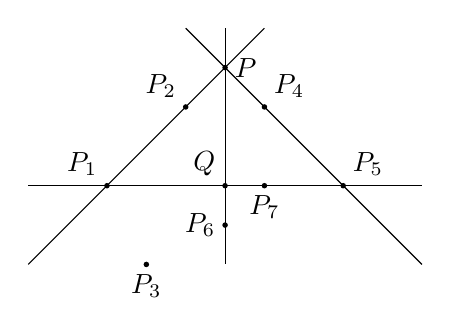
\begin{tikzpicture}
    \node (P1) at (0cm,0cm) {};
    \node (P2) at (1cm,1cm) {};
    \node (P3) at (0.5cm,-1cm) {};
    \node (P4) at (2cm,1cm) {};
    \node (P5) at (3cm,0cm) {};
    \node (P6) at (1.5cm,-0.5cm) {};
    \node (P7) at (2cm,0cm) {};
    \draw (-1cm,-1cm) -- (2cm,2cm);
    \draw (1.5cm,2cm) -- (1.5cm,-1cm);
    \draw (1cm,2cm) -- (4cm,-1cm);
    \draw (-1cm,0cm) -- (4cm,0cm);
    \node (P) at (1.5cm,1.5cm) {};
    \node (Q) at (1.5cm,0cm) {};
    
    \node[anchor=south east] at (P1) {\(P_1\)};
    \node[anchor=south east] at (P2) {\(P_2\)};
    \node[anchor=north] at (P3) {\(P_3\)};
    \node[anchor=south west] at (P4) {\(P_4\)};
    \node[anchor=south west] at (P5) {\(P_5\)};
    \node[anchor=east] at (P6) {\(P_6\)};
    \node[anchor=north] at (P7) {\(P_7\)};
    \node[anchor=west] at (P) {\(P\)};
    \node[anchor=south east] at (Q) {\(Q\)};
    \fill \foreach \s in {P1, P2, P3, P4, P5, P6, P7, P, Q}{(\s) circle [radius=1pt]};
  \end{tikzpicture}
  \caption{Example of constructible points}\label{fig:constructible}
\end{figure}

\paragraph{Observations.}
\begin{enumerate}[label=(\arabic*)]
  \item We can draw a line passing through \(P \in K_n\) which is perpendicular to a line \(l\) through \(Q \in K_n\). See \autoref{fig:perpendicularline}.
  \begin{figure}[ht]\centering
    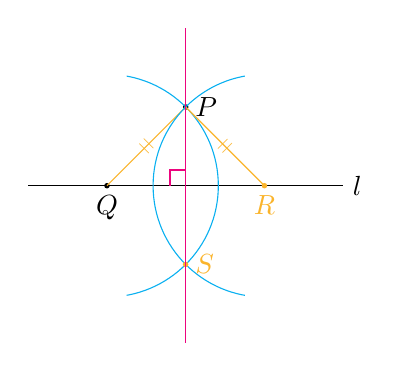
\begin{tikzpicture}
      \draw[name path=linel] (-2cm,0cm) -- (2cm,0cm);
      \node[anchor=west] at (2cm,0cm) {\(l\)};
      \coordinate (P) at (0cm,1cm);
      \coordinate (Q) at (-1cm,0cm);
      \fill foreach \s in {P,Q}{(\s) circle [radius=1pt]};
      \node[anchor=west] at (P) {\(P\)};
      \node[anchor=north] at (Q) {\(Q\)};
      
      \begin{scope}
        \clip (-.75cm,-1.5cm) rectangle (1cm,1.5cm);
        \draw[myblue, name path global=Qcircle] (Q) circle [radius=1.4142cm];
      \end{scope}
      
      \coordinate (R) at (1cm,0cm);
      \fill[myyellow] (R) circle [radius=1pt];
      \node[anchor=north, myyellow] at (R) {\(R\)};
      
      \path[draw, myyellow] (Q) -- node[rotate=45]{\tiny\(||\)} (P) -- node[rotate=-45]{\tiny\(||\)} (R);
      
      \begin{scope}
        \clip (-1cm,-1.5cm) rectangle (.75cm,1.5cm);
        \draw[myblue, name path global=Rcircle] (R) circle [radius=1.4142cm];
      \end{scope}
      
      \coordinate (O) at (0cm,0cm) pic[draw=myred, angle radius=2mm]{right angle=P--O--Q};
      
      \fill[myyellow, name intersections={of=Qcircle and Rcircle, by={temp,S}}] (S) circle [radius=1pt];
      \node[myyellow, anchor=west] at (S) {\(S\)};
      
      \draw[myred] (0cm,2cm) -- (0cm,-2cm);
    \end{tikzpicture}
    \caption{Drawing a line passing through \(P\) perpendicular to \(l\)}\label{fig:perpendicularline}
  \end{figure}
  \begin{enumerate}[nosep]
    \item Draw a circle centered at \(Q\) whose radius is \(|\overline{PQ}|\).
    \item Let \(R\) be a point on \(l\) such that \(|\overline{PQ}| = |\overline{PR}|\).
    \item Draw a circle centered at \(R\) whose radius is \(|\overline{PR}|\).
    \item Let \(S \neq P\) be an intersection of the two circles.
    \item Draw a line passing through \(P\) and \(S\).
  \end{enumerate}
  
  \item We can draw a line parallel to \(l\) containing \(P \in K_n\). See \autoref{fig:parallelline}.
  \begin{figure}[ht]\centering
    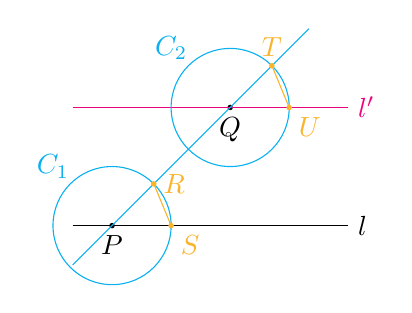
\begin{tikzpicture}
      \draw[name path=linel] (0cm,0cm) -- (3.5cm,0cm); % Given
      \node[anchor=west] at (3.5cm,0cm) {\(l\)};
      \node (P) at (0.5cm,0cm) {};
      \node (Q) at (2cm,1.5cm) {};
      \node[anchor=north] at (P) {\(P\)};
      \node[anchor=north] at (Q) {\(Q\)};
      \fill (P) circle [radius=1pt]; % Given
      \fill (Q) circle [radius=1pt]; % Given
      
      \draw[myred, name path=linelp] (0cm,1.5cm) -- (3.5cm,1.5cm);
      \node[myred, anchor=west] at (3.5cm,1.5cm) {\(l'\)};
      \draw[myblue, name path=diag] (0cm,-0.5cm) -- (3cm,2.5cm);
      
      \draw[myblue, name path=Pcircle] (P) circle [radius=0.75cm];
      \draw[myblue, name path=Qcircle] (Q) circle [radius=0.75cm];
      \path[myblue] (P) ++ (-.75cm,.75cm) node {\(C_1\)};
      \path[myblue] (Q) ++ (-.75cm,.75cm) node {\(C_2\)};
      
      \fill[myyellow, name intersections={of=Pcircle and diag, by={R}}] (R) circle [radius=1pt];
      \fill[myyellow, name intersections={of=Pcircle and linel, by={S}}] (S) circle [radius=1pt];
      \node[myyellow, anchor=west] at (R) {\(R\)};
      \node[myyellow, anchor=north west] at (S) {\(S\)};
      \draw[myyellow] (R) -- (S);
      
      \fill[myyellow, name intersections={of=Qcircle and diag, by={T,temp}}] (T) circle [radius=1pt];
      \fill[myyellow, name intersections={of=Qcircle and linelp, by={temp,U}}] (U) circle [radius=1pt];
      \node[myyellow, anchor=south] at (T) {\(T\)};
      \node[myyellow, anchor=north west] at (U) {\(U\)};
      \draw[myyellow] (T) -- (U);
    \end{tikzpicture}
    \caption{Drawing a line parallel to \(l\)}\label{fig:parallelline}
  \end{figure}
  \begin{enumerate}[nosep]
    \item Draw the line \(\overline{PQ}\).
    \item Choose a point \(R\) on \(\overline{PQ}\).
    \item Draw a circle \(C_1\) centered at \(P\) whose radius is \(|\overline{PR}|\).
    \item Draw a circle \(C_2\) centered at \(Q\) whose radius is \(|\overline{PR}|\).
    \item let \(T\) be an intersection of the circle \(C_2\) and the line \(m\).
    \item let \(U\) be a point on \(C_2\) such that \(|\overline{TU}| = |\overline{RS}|\).
    \item Draw a line \(l'\) which passes through \(Q\) and \(U\).
  \end{enumerate}
  
  \item Given two rays of angles \(\theta\) and \(\phi\), we can construct rays of angles \(\theta \pm \phi\), \(-\theta\), and \(\theta/2\). See \autoref{fig:raybisectingangle}.
  \begin{figure}[ht]
    \centering
    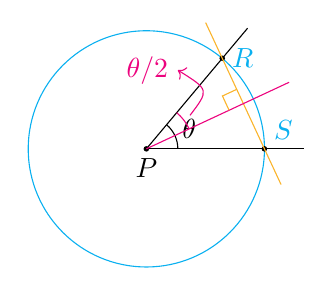
\begin{tikzpicture}[extended line/.style={shorten >=-.5cm,shorten <=-.5cm}]
      \coordinate (P) at (0cm,0cm);
      \node[anchor=north] at (P) {\(P\)};
      \coordinate (t1) at (0:2cm);
      \coordinate (t2) at (50:2cm);
      \draw[name path=ray1] (t1) -- (P);
      \draw[name path=ray2] (t2) -- (P);
      \path (t1) -- (P) -- (t2) pic[draw, angle radius=4mm, "\(\theta\)", angle eccentricity=1.5] {angle = t1--P--t2};
      \fill (P) circle [radius=1pt];
      
      \draw[name path=Pcircle, myblue] (P) circle [radius=1.5cm];
      \fill[name intersections={of=ray1 and Pcircle, by={S}}] (S) circle [radius=1pt];
      \fill[name intersections={of=ray2 and Pcircle, by={R}}] (R) circle [radius=1pt];
      \node[myblue, anchor=west] at (R) {\(R\)};
      \node[myblue, anchor=south west] at (S) {\(S\)};
      \draw[myyellow, extended line, name path=RS] (R) -- (S);
      \draw[myred, name path=T3] (P) -- (25:2cm) coordinate (t3) pic[draw=myred, angle radius=6mm] {angle = t3--P--t2};
      \path[name intersections={of=RS and T3, by=X}] (X) pic[draw=myyellow, angle radius=2mm]{right angle=R--X--P};
      \draw[->, myred] (37.5:7mm) .. controls (.8cm,.75cm) .. (.4cm,1cm) node[anchor=east]{\(\theta/2\)};
    \end{tikzpicture}
    \caption{Drawing a ray of angle \(\theta/2\)}\label{fig:raybisectingangle}
  \end{figure}
  
  For example, we can draw a ray of angle \(\theta/2\) as follows:
  \begin{enumerate}[nosep]
    \item Draw a circle centered at \(P\).
    \item Let \(R\) and \(S\) be the intersections of the rays with the circle.
    \item Draw a line passing through \(R\) and \(S\).
    \item By (1), we can draw a line containing \(P\) perpendicular to \(\overline{RS}\).
  \end{enumerate}
\end{enumerate}

As \(P_1, \dots, P_n\) are in the plane, we may assume that \(P_j = z_j = x_j + y_ji \in \C\) and \(z_1 = 0\), \(z_2 = 1\). We set \(K_n \coloneq K(z_1, \dots, z_n) \in \C\).

\begin{lemma}
  \begin{enumerate}[label=\textup{(\arabic*)}, nosep]
    \item For any \(n \in \Z\), \(n\) and \(ni\) are in \(K_n\).
    \item \(z = x + yi \in K_n\) if and only if \(x, yi \in K_n\).
  \end{enumerate}
\end{lemma}

\begin{proof}
  (1) We need to show that \((n,0)\) and \((0,n)\) are constructible. We use induction on \(n\). To show that \((n,0) \in K_n\), draw a circle centered at \((n-1,0)\) with radius \(1\). One of the intersections of \(x\)-axis with the circle is the point \((n,0)\). See \autoref{fig:n0inkn}.
  
  To show that \((0,n) \in K_n\), first draw a circle centered at \(z_1 = (0,0)\) passing through \(z_2\). One of the intersections of the circle and the \(y\)-axis is the point \((0,1)\). Now, draw a circle centered at \((0,n-1)\) with radius \(1\). One of the intersections of \(y\)-axis with the circle is the point \((0,n)\). see \autoref{fig:0ninkn}.
  \begin{figure}[ht]
    \centering
    \begin{subfigure}{8cm}
      \centering
      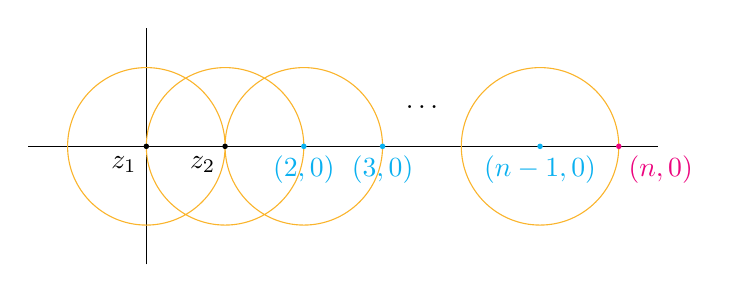
\begin{tikzpicture}
        \draw (-1.5cm,0cm) -- (6.5cm,0cm);
        \draw (0cm,-1.5cm) -- (0cm,1.5cm);
        \node[anchor=north east] at (0cm,0cm) {\(z_1\)};
        \node[anchor=north east] at (1cm,0cm) {\(z_2\)};
        \node[myblue,anchor=north] at (2cm,0cm) {\((2,0)\)};
        \node[myblue,anchor=north] at (3cm,0cm) {\((3,0)\)};
        \node[myblue,anchor=north] at (5cm,0cm) {\((n-1,0)\)};
        \node[myred,anchor=north west] at (6cm,0cm) {\((n,0)\)};
        \draw[myyellow] foreach \s in {0,1,2,5}{(\s cm,0cm) circle [radius=1cm]};
        \fill foreach \s in {0,1}{(\s cm,0cm) circle [radius=1pt]};
        \fill[myblue] foreach \s in {2,3,5}{(\s cm,0cm) circle [radius=1pt]};
        \fill[myred] (6cm,0cm) circle [radius=1pt];
        \node at (3.5cm,0.5cm) {\(\dots\)};
      \end{tikzpicture}
      \caption{Proof of \((n,0) \in K_n\)}\label{fig:n0inkn}
    \end{subfigure}\qquad
    \begin{subfigure}{3cm}
      \centering
      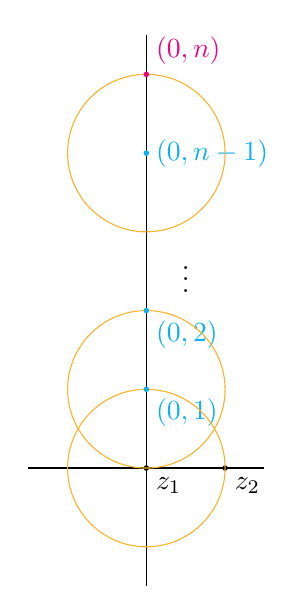
\begin{tikzpicture}
        \draw (-1.5cm,0cm) -- (1.5cm,0cm);
        \draw (0cm,-1.5cm) -- (0cm,5.5cm);
        \path foreach \s in {1,2}{(0cm,\s cm) node[myblue,anchor=north west]{\((0,\s)\)}};
        \node[anchor=north west] at (0cm,0cm) {\(z_1\)};
        \node[anchor=north west] at (1cm,0cm) {\(z_2\)};
        \fill foreach \s in {0,1}{(\s cm,0cm) circle [radius=1pt]};
        \node[myblue,anchor=west] at (0cm,4cm) {\((0,n-1)\)};
        \node[myred,anchor=south west] at (0cm,5cm) {\((0,n)\)};
        \draw[myyellow] foreach \s in {0,1,4}{(0cm,\s cm) circle [radius=1cm]};
        \fill[myblue] foreach \s in {1,2,4}{(0cm,\s cm) circle [radius=1pt]};
        \fill[myred] (0cm,5cm) circle [radius=1pt];
        \node at (0.5cm,2.5cm) {\(\vdots\)};
      \end{tikzpicture}
      \caption{Proof of \((0,n) \in K_n\)}\label{fig:0ninkn}
    \end{subfigure}
    \caption{Proof of Lemma 11.1(1)}\label{fig:lem11.1(1)}
  \end{figure}
  
  \newclass{22-11-23}
  (2) \((\Rightarrow)\) Assume \(x+yi \in K_n\). Draw a line passing \((x,y)\) and perpendicular to each axis. Find the intersection of each line with the axis. Therefore, \(x = (x,0)\) and \(y = (0,y)\) are in \(K_n\). See \autoref{fig:lem11.1(2)a}.
  
  \((\Leftarrow)\) Assume that \((x,0), (0,y) \in K_n\). Draw a line passing \((x,0)\) and perpendicular to \(x\)-axis. Draw a line passing \((0,y)\) and perpendicular to \(y\)-axis. Find the intersection of the two lines. Therefore, we get that \((x,y) \in K_n\). See \autoref{fig:lem11.1(2)b}.
  \begin{figure}[ht]
    \centering
    \begin{subfigure}{5cm}
      \centering
      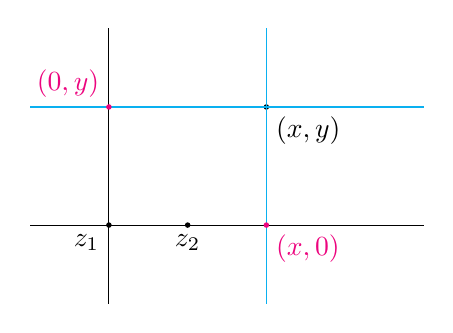
\begin{tikzpicture}
        \draw (-1cm,0cm) -- (4cm,0cm) (0cm,2.5cm) -- (0cm,-1cm);
        \coordinate (z1) at (0cm,0cm);
        \coordinate (z2) at (1cm,0cm);
        \fill (z1) circle [radius=1pt];
        \fill (z2) circle [radius=1pt];
        \node[anchor=north east] at (z1) {\(z_1\)};
        \node[anchor=north] at (z2) {\(z_2\)};
        
        \coordinate (z) at (2cm,1.5cm);
        \fill (z) circle [radius=1pt];
        \node[anchor=north west] at (z) {\((x,y)\)};
        
        \draw[myblue] (2cm,2.5cm) -- (2cm,-1cm) (-1cm,1.5cm) -- (4cm,1.5cm);
        
        \coordinate (x) at (2cm,0cm);
        \coordinate (y) at (0cm,1.5cm);
        \fill[myred] (x) circle [radius=1pt];
        \fill[myred] (y) circle [radius=1pt];
        \node[myred, anchor=north west] at (x) {\((x,0)\)};
        \node[myred, anchor=south east] at (y) {\((0,y)\)};
      \end{tikzpicture}
      \caption{Proof of \((x,0),(0,y) \in K_n\)}\label{fig:lem11.1(2)a}
    \end{subfigure}\qquad
    \begin{subfigure}{5cm}
      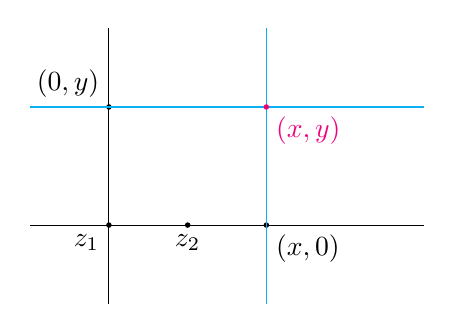
\begin{tikzpicture}
        \draw (-1cm,0cm) -- (4cm,0cm) (0cm,2.5cm) -- (0cm,-1cm);
        \coordinate (z1) at (0cm,0cm);
        \coordinate (z2) at (1cm,0cm);
        \fill (z1) circle [radius=1pt];
        \fill (z2) circle [radius=1pt];
        \node[anchor=north east] at (z1) {\(z_1\)};
        \node[anchor=north] at (z2) {\(z_2\)};
        \coordinate (x) at (2cm,0cm);
        \coordinate (y) at (0cm,1.5cm);
        \fill (x) circle [radius=1pt];
        \fill (y) circle [radius=1pt];
        \node[anchor=north west] at (x) {\((x,0)\)};
        \node[anchor=south east] at (y) {\((0,y)\)};
        
        \draw[myblue] (2cm,2.5cm) -- (2cm,-1cm) (-1cm,1.5cm) -- (4cm,1.5cm);
        
        \coordinate (z) at (2cm,1.5cm);
        \fill[myred] (z) circle [radius=1pt];
        \node[myred, anchor=north west] at (z) {\((x,y)\)};
      \end{tikzpicture}
      \caption{Proof of \((x,y) \in K_n\)}\label{fig:lem11.1(2)b}
    \end{subfigure}
    \caption{Proof of Lemma 11.1(2)}\label{fig:lem11.1(2)}
  \end{figure}
\end{proof}

\begin{proposition}
  Suppose \(n \geq 2\) and let \(K_n = K(z_1, \dots, z_n)\), where \(z_1 = 0\) and \(z_2 = 1\). Then, \(K_n\) is a subfield of \(\C\) satisfying
  \[ \text{If \(z \in K_n\), then \(\sqrt z\) and \(\bar z\) are in \(K_n\).} \tag{\(*\)} \]
  If \(E\) is a subfield of \(\C\) containing \(z_1, \dots, z_n\) satisfying \((*)\), then \(K_n \subset E\).
\end{proposition}

\begin{proof}
  \emph{Step 1.} We show that \(K_n\) is a subfield of \(\C\).
  
  Let \(z = a+bi\) and \(w = c+di\) be two points in \(K_n\). Then,
  \begin{align*}
    z \pm w & = (a \pm c) + (b \pm d)i, \\
    zw & = (ac-bd) + (ad+bc)i, \\
    \frac1z & = \frac1{a^2+b^2}(a-bi).
  \end{align*}
  By Lemma 11.1(2), it suffices to show that
  \begin{enumerate}[label=(\roman*),nosep]
    \item if \((a,0)\) and \((b,0)\) are constructible, then \((a+b,0)\) is constructible.
    \item if \((a,0)\) and \((b,0)\) are constructible, then \((ab,0)\) is constructible.
    \item If \((a,0)\) is constructible, then \((1/a,0)\) is constructible.
  \end{enumerate}
  
  For (i), draw a line \(l\) passing \((0,1)\) and \((a,0)\). Draw a line passing through \((b,0)\) and perpendicular to the \(x\)-axis. Draw a line passing through \((0,1)\) and perpendicular to the \(y\)-axis. Let \(X\) be the intersection of these two orthogonal lines. Draw a line \(l'\) passing through \(X\) and parallel to \(l\). The intersection of \(l'\) and the \(x\)-axis is the point \((a+b,0)\), because the distance from this point to \((b,0)\) is \(a\). See \autoref{fig:prop11.2a}.
  \begin{figure}[ht]
    \centering
    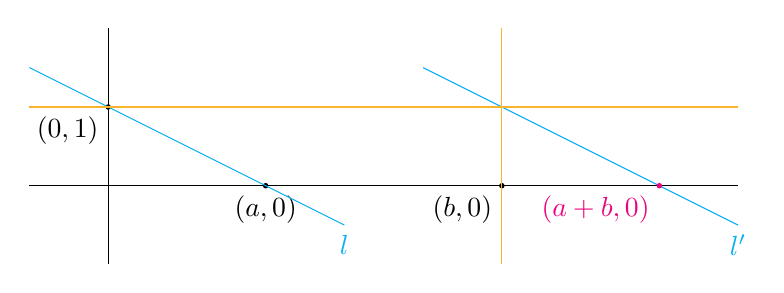
\begin{tikzpicture}
      \draw (-1cm,0cm) -- (8cm,0cm) (0cm,-1cm) -- (0cm,2cm);
      \coordinate (a0) at (2cm,0cm);
      \coordinate (b0) at (5cm,0cm);
      \coordinate (01) at (0cm,1cm);
      \fill foreach \s in {a0,01,b0}{(\s) circle [radius=1pt]};
      \node[anchor=north] at (a0) {\((a,0)\)};
      \node[anchor=north east] at (b0) {\((b,0)\)};
      \node[anchor=north east] at (01) {\((0,1)\)};
      
      \draw[myblue] (-1cm,1.5cm) -- (3cm,-0.5cm) (4cm,1.5cm) -- (8cm,-0.5cm);
      \node[myblue, anchor=north] at (3cm,-0.5cm) {\(l\)};
      \node[myblue, anchor=north] at (8cm,-0.5cm) {\(l'\)};
      \draw[myyellow] (5cm,2cm) -- (5cm,-1cm) (-1cm,1cm) -- (8cm,1cm);
      
      \coordinate (ab0) at (7cm,0cm);
      \fill[myred] (ab0) circle [radius=1pt];
      \node[myred, anchor=north east] at (ab0) {\((a+b,0)\)};
    \end{tikzpicture}
    \caption{Proof of \((a+b,0) \in K_n\)}\label{fig:prop11.2a}
  \end{figure}
  
  For (ii), draw a line \(l\) connecting \((0,a)\) and \((1,0)\). Since \((b,0)\) is in \(K_n\), \((1+b,0)\) is also in \(K_n\) by (i). Draw a line \(l'\) passing through \((1+b,0)\) and parallel to \(l\). Let \((0,y)\) be the \(y\)-section of \(l'\). Comparing the inclination, we have that
  \[ \frac a1 = \frac y{1+b} \qquad \text{or} \qquad y = a+ab. \]
  It gives that \((0,y) = (0,a+ab) \in K_n\). By (i), we have that \((0,ab) \in K_n\), or \((ab,0) \in K_n\). See \autoref{fig:prop11.2b}.
  \begin{figure}[ht]
    \centering
    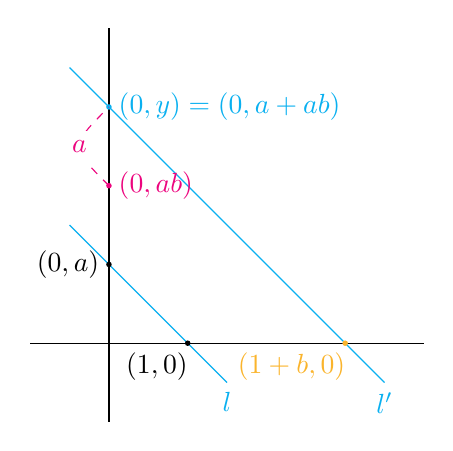
\begin{tikzpicture}
      \draw (-1cm,0cm) -- (4cm,0cm) (0cm,-1cm) -- (0cm,4cm);
      \coordinate (z2) at (1cm,0cm);
      \coordinate (0a) at (0cm,1cm);
      \draw[myblue] (-0.5cm,1.5cm) -- (1.5cm,-0.5cm);
      \node[myblue, anchor=north] at (1.5cm,-0.5cm) {\(l\)};
      \coordinate (1b0) at (3cm,0cm);
      \coordinate (0x) at (0cm,3cm);
      \draw[myblue] (-0.5cm,3.5cm) -- (3.5cm,-0.5cm);
      \node[myblue, anchor=north] at (3.5cm,-0.5cm) {\(l'\)};
      \fill foreach \s in {z2,0a}{(\s) circle [radius=1pt]};
      \fill[myyellow] (1b0) circle [radius=1pt];
      \fill[myblue] (0x) circle [radius=1pt];
      
      \node[anchor=north] at (z2) {\llap{\((1,0)\)}};
      \node[anchor=east] at (0a) {\((0,a)\)};
      \node[anchor=north, myyellow] at (1b0) {\llap{\((1+b,0)\)}};
      \node[myblue, anchor=west] at (0x) {\((0,y) = (0,a+ab)\)};
      
      \coordinate (0ab) at (0cm,2cm);
      \fill[myred] (0ab) circle [radius=1pt];
      \node[myred, anchor=west] at (0ab) {\((0,ab)\)};
      \draw[myred, dashed] (0ab) .. controls (-.5cm,2.5cm) .. node[fill=white]{\(a\)} (0x);
    \end{tikzpicture}
    \caption{Proof of \((ab,0) \in K_n\)}\label{fig:prop11.2b}
  \end{figure}
  
  For (iii), draw a line \(l\) connecting \((0,a)\) and \((1,0)\). Since \((0,a)\) is in \(K_n\), \((0,1+a)\) is also in \(K_n\) by (i). Draw a line \(l'\) passing through \((0,1+a)\) and parallel to \(l'\). Let \((x,0)\) be the \(x\)-section of \(l'\). Comparing the inclination, we have that
  \[ \frac a1 = \frac{1+a}x \qquad \text{or} \qquad x = \frac1a + 1. \]
  It gives that \((x,0) = (1/a+1,0) \in K_n\). By (i), we have that \((1/a,0) \in K_n\). See \autoref{fig:prop11.2c}.
  \begin{figure}[ht]
    \centering
    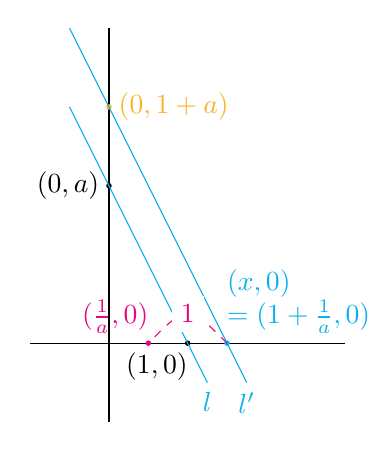
\begin{tikzpicture}
      \draw (-1cm,0cm) -- (3cm,0cm) (0cm,-1cm) -- (0cm,4cm);
      \coordinate (z2) at (1cm,0cm);
      \coordinate (0a) at (0cm,2cm);
      \node[anchor=north] at (z2) {\llap{\((1,0)\)}};
      \node[anchor=east] at (0a) {\((0,a)\)};
      \fill foreach \s in {z2,0a}{(\s) circle [radius=1pt]};
      \draw[myblue] (-0.5cm,3cm) -- (1.25cm,-0.5cm);
      \node[myblue, anchor=north] at (1.25cm,-0.5cm) {\(l\)};
      
      \fill[myyellow] (0cm,3cm) circle [radius=1pt];
      \node[myyellow, anchor=west] at (0cm,3cm) {\((0,1+a)\)};
      \draw[myblue] (-0.5cm,4cm) -- (1.75cm,-0.5cm);
      \node[myblue, anchor=north] at (1.75cm,-0.5cm) {\(l'\)};
      
      \fill[myblue] (1.5cm,0cm) circle [radius=1pt];
      \node[myblue, anchor=south, align=left] at (1.5cm,0cm) {\rlap{\((x,0)\)}\\\rlap{\(= (1+\frac1a,0)\)}};
      
      \draw[dashed,myred] (1.5cm,0cm) .. controls (1cm,0.5cm) .. node[fill=white]{\(1\)} (0.5cm,0cm) node[anchor=south]{\llap{\((\frac1a,0)\)}};
      \fill[myred] (0.5cm,0cm) circle [radius=1pt];
    \end{tikzpicture}
    \caption{Proof of \((1/a) \in K_n\)}\label{fig:prop11.2c}
  \end{figure}
  
  \smallskip
  
  \emph{Step 2.} We show that \(K_n\) satisfies \((*)\).
  
  We snow if \(z \in K_n\), then \(\sqrt z \in K_n\). Write \(z = a+b\sqrt{-1} = r e^{i\theta} = r(\cos\theta i\sin\theta)\), where \(r^2 = a^2+b^2\). Then, we get
  \[ \sqrt z = \sqrt r \, e^{i \theta/2}. \]
  We first show that if \((a,0) \in K_n\), then \((\sqrt a,0) \in K_n\).
  \begin{figure}[ht]
    \centering
    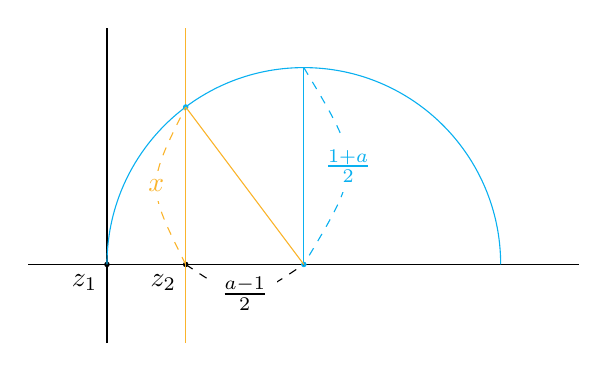
\begin{tikzpicture}
      \draw (-1cm,0cm) -- (6cm,0cm) (0cm,-1cm) -- (0cm,3cm);
      \coordinate (z1) at (0cm,0cm);
      \coordinate (z2) at (1cm,0cm);
      \fill foreach \s in {z1,z2}{(\s) circle [radius=1pt]};
      \node[anchor=north east] at (z1) {\(z_1\)};
      \node[anchor=north east] at (z2) {\(z_2\)};
      \coordinate (c) at (2.5cm,0cm);
      \fill[myblue] (c) circle [radius=1pt];
      \draw[dashed] (z2) .. controls (1.75cm,-.5cm) .. node[fill=white]{\(\frac{a-1}2\)} (c);
      \draw[myblue, name path = circle] (5cm,0cm) arc (0:180:2.5cm);
      \draw[myyellow, name path = line] (1cm,-1cm) -- (1cm,3cm);
      \fill[myblue, name intersections={of=circle and line,by=x}] (x) circle [radius=1pt];
      \draw[myblue] (2.5cm,2.5cm) -- (c);
      \draw[myblue, dashed] (2.5cm,2.5cm) .. controls (3.25cm,1.25cm) .. node[fill=white]{\(\frac{1+a}2\)} (c);
      \draw[myyellow] (x)--(c);
      \draw[myyellow, dashed] (z2) .. controls (0.5cm,1cm) .. node[fill=white]{\(x\)} (x);
    \end{tikzpicture}
    \caption{Proof of \((\sqrt a,0) \in K_n\)}\label{fig:sqrtisconstructible}
  \end{figure}
  The point \(((1+a)/2,0)\) is in \(K_n\), by (i), (ii), and (iii). See \autoref{fig:sqrtisconstructible}.
  
  Since
  \[ \left( \frac{1+a}2 \right)^2 = x^2 + \left( \frac{a-1}2 \right)^2, \]
  we get that \(x = \sqrt a\). It gives that \((1,\sqrt a) \in K_n\), so \((\sqrt a,0) \in K_n\). If \(r = \sqrt{a^2+b^2} \in K_n\), then \(r^{-1}z = e^{i\theta} \in K_n\). By Observations, we get \(e^{i\theta/2} \in K_n\). Therefore, we conclude that \(\sqrt z = \sqrt r e^{i\theta/2} \in K_n\).
  
  If \(z = a+bi \in K_n\), then \(\bar z = a-bi \in K_n\), as \((0,b) \in K_n\).
  
  \smallskip
  
  \emph{Step 3.} We show that \(K_n \subset E\) if \(E\) satisfies \((*)\).
  
  It suffices to show that the points obtained as in \(\star\) are contained in \(E\), i.e., for each of the following, the intersection points are in \(E\).
  \begin{align*}
    \text{(i) } & \begin{cases} ax+by+c = 0 \\ a'x+b'y+c' = 0 \end{cases} \\
    \text{(ii) } & \begin{cases} ax+by+c = 0 \\ (x-a')^2 + (y-b')^2 = c^2 \end{cases} \\
    \text{(iii) } & \begin{cases} (x-a)^2 + (y-b) = c^2 \\ (x-a')^2 + (y-b') = c'^2 \end{cases}
  \end{align*}
  To show (i), it is enough to check \(a,b,c \in E\) as \(E\) is a field. Now we show this.
  
  Let \(z = x_1+y_1\sqrt i\) and \(w = x_2+y_2\sqrt i\) are points in \(E\) such that the line through \(z\) and \(w\) is given by \(ax+by+c = 0\). As
  \[ \bar z = x_1 - y_1 i \in E \qquad \text{and} \qquad \frac{z+\bar z}2 = x_1 \in E, \]
  thus
  \[ \frac{\bar z i - zi}2 = y_i \in E. \]
  Hence, \(x_1, y_1, x_2, y_2 \in E\). It gives that
  \[ \frac{y_2-y_1}{x_2-x_1} (x-x_1) = y-y_1, \]
  which implies that \(a,b,c \in E\) in \(ax+by+c=0\).
  
  Similarly, one can easily check (ii) and (iii).
\end{proof}

\begin{recall}
  A field extension \(E/F\) is \(2\)-radical if there exists a chain
  \[ F \subset F(\alpha_1) \subset F(\alpha_1,\alpha_2) \subset \cdots \subset F(\alpha_1, \dots, \alpha_n) = E \]
  such that \(\alpha_1^2 \in F\) and \(\alpha_i^2 \in F(\alpha_1,\dots,\alpha_{i-1})\) for each \(i \geq 2\).
\end{recall}

\begin{theorem}
  Let \(F = \Q(z_1, \dots, z_n, \bar z_1, \dots, \bar z_n)\), where \(z_i \in \C\), \(z_1 = 0\), and \(z_2 = 1\). Then, \(z \in K_n\) if and only if there exists a \(2\)-radical extension \(E/F\) with \(z \in E\), where \(K_n = K(z_1, \dots, z_n)\).
\end{theorem}

\begin{proof}
  Let
  \[ L = \{z \in \C \mid \text{there exists a \(2\)-radical extension \(E/F\) with \(z \in E\)}\}. \]
  We show \(L = K_n\). By Proposition 11.2, \(\bar z_n \in K_n\) for each \(i\), so \(F \in K_n\). Let \(z \in L\). Then, there exists a chain
  \[ F \subset F(\alpha_1) \subset \cdots \subset F(\alpha_1, \dots, \alpha_n) = E \]
  with \(\alpha_1^2 \in F\) and \(\alpha_i^2 \in F(\alpha_1, \dots, \alpha_{i-1})\) for each \(i \geq 2\). As \(\alpha_1^2 \in F \subset K_n\), Proposition 11.2 gives that \(\alpha_1 \in K_n\). For \(i \geq 2\), as \(\alpha_i^2 \in F(\alpha_1, \dots, \alpha_{i-1}) \subset K_n\), Proposition 11.2 gives that \(\alpha_i \in K_n\). Hence, we get that \(L \subset K_n\).
  
  Now we show \(K_n \subset L\). By Proposition 11.2, it suffices to show that \(L\) is a field satisfying \((*)\). Let \(z_1, z_2 \in L\). Then there exist \(2\)-radical Extensions \(E_1/F\) and \(E_2/F\) with \(z_i \in E_i\), \(i=1,2\). Then, \(E_1 E_2/F\) is a \(2\)-radical extension containing \(z_1z_2\), \(z_1\pm z_2\), and \(1/z_1\). As \(E_1E_2 \subset L\), \(L\) is a field. Since \(E_1(\sqrt{z_1})/E_1\) is a \(2\)-radical extension, so is \(E_1(\sqrt{z_1})/F\), thus \(\sqrt{z_1} \in L\). As \(F = \bar F\) (conjugate of \(F\), i.e., \(\bar F = \{\bar a \mid a \in F\}\)), \(\bar E_1 / F = \bar F\) is a \(2\)-radical extension, so \(\bar z_1 \in L\).
\end{proof}

\begin{corollary}
  Let \(z \in K_n\). Then, \(z\) is algebraic over \(F\), where \(F = \Q(z_1, \dots, z_n, \bar z_1, \dots, \bar z_n)\) and \([F(z):F] = 2^m\) for some \(m \geq 0\).
\end{corollary}

\begin{proof}
  By Theorem 11.3, there exists a \(2\)-radical extension \(E/F\) with \(z \in E\). Hence, \([F(z):F] \mid [E:F] = 2^k\) for some positive integer \(k\).
\end{proof}

\paragraph{Question 1.} Given a cube with volume \(1\), can we construct a cube with volume \(2\)? Equivalently, given \(z_1 = 0\) and \(z_2 = 1\), is \(\sqrt[3]2 \in K_2\) holds?

No, it is impossible, as \([\Q(\sqrt[3]2) : \Q] = 3\) by Corollary 11.4.

\paragraph{Question 2.} Can we construct a square whose area is \(\pi\)? Equivalently, given \(z_1 = 0\) and \(z_2 = 1\), is \(\sqrt\pi \in K_2\) holds?

No, as \(\pi\) is transcendental over \(\Q\), so by Corollary 11.4, we get that \(\sqrt\pi \notin K_2\).

\paragraph{Question 3.} Can we trisect an angle? Equivalently, given \(z_1 = 0\), \(z_2 = 1\), and \(z_3 = \cos\theta\), is \(\cos(\theta/3) \in K_3\) holds?

Let \(F = \Q(\cos\theta)\). From
\[ \cos\theta = 4 \cos^3 \left(\frac\theta3\right) - 3 \cos \left(\frac\theta3\right), \]
\(\cos(\theta/3)\) is a root of \(f = 4x^3 - 3x - \cos\theta \in F[x]\). Observe that
\begin{quote}
  \(f\) is reducible over \(F\) \\
  if and only if \(f\) has a root in \(F\) \\
  if and only if for any root \(\alpha\) of \(f\), we have that \([F(\alpha):F] \leq 2\) \\
  if and only if \(\cos(\theta/3) \in K_3\).
\end{quote}

In particular, if \(\theta=\pi/3\), then we get \(f = 4x^3 - 3x + 1/2\), which is irreducible over \(F\). Thus, \(\pi/3\) cannot be trisected. But, if \(\theta = \pi/2\), then we get \(f = 4x^3 - 3x\) is reducible, thus \(\pi/2\) can be trisected.

\paragraph{Question 4.} Can we construct a regular \(n\)-gon? Equivalently, given \(z_1=0\) and \(z_2=1\), is \(\eta_n = \cos(2\pi/n) + i \sin(2\pi/n) \in K_2\) holds?

For example, a regular \(3\)-gon is an equilateral triangle, and a regular \(4\)-gon is a square. See \autoref{fig:3gon} for constructing a regular \(3\)-gon.
\begin{figure}[ht]
  \centering
  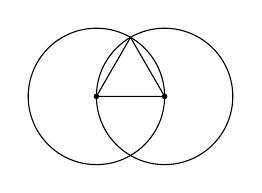
\begin{tikzpicture}
    \draw (210:0.5cm) circle [radius=0.8660cm];
    \draw (-30:0.5cm) circle [radius=0.8660cm];
    \fill (-30:0.5cm) circle [radius=1pt];
    \fill (210:0.5cm) circle [radius=1pt];
    \draw (-30:0.5cm) -- (210:0.5cm) -- (90:0.5cm) -- cycle;
  \end{tikzpicture}
  \caption{Constructing an equilateral triangle}\label{fig:3gon}
\end{figure}

\paragraph{Observations.}
\begin{enumerate}
  \item If \(n = 2^m\), then \(\eta_n \in K_2\), thus a regular \(2^m\)-gon can be constructed. \par
  If \(m=2\), then \(\eta_4 \in K_2\). Use induction on \(m\). Assume \(\eta_{2^m} \in K_2\). Then by drawing a bisecting line, we get that \(\eta_{2^{m+1}} \in K_2\).
  
  \item \(\eta_n \in K_2\) if and only if \(\eta_{2n} \in K_2\), as angles can be doubled or bisected.
  
  \item Let \(\gcd(m,n) = 1\). Then, \(\eta_{mn} \in K_2\) if and only if \(\eta_n, \eta_m \in K_2\). \par
  Since \(2\pi/n = n \cdot (2\pi/mn)\) and \(2\pi/n = m \cdot (2\pi/mn)\), the right direction holds. Since there exists some integer \(a\) and \(b\) such that \(1=am+bn\), we have \(2\pi/mn = a \cdot (2\pi/n) + b \cdot (2\pi/m)\). Thus the left direction holds.
\end{enumerate}

\begin{lemma}
  Let \(F\) be a field of characteristic zero, and let \(L/F\) be a normal extension. Then, \(L/F\) is \(2\)-radical if and only if \([L:F] = 2^m\) for some \(m \geq 0\).
\end{lemma}

\begin{proof}
  (\(\Rightarrow\)) It follows from the definition of \(2\)-radical extension.
  
  (\(\Leftarrow\)) Let \([L:F] = 2^m\) and \(G = \Gal(L/F)\) with \(|G| = 2^m\). By Sylow's theorem, there exists some \(H < G\) with \(|H| = 2^{m-1}\). Since \([G:H] = 2\), \(H \vartriangleleft G\), thus \([L^H:F] = 2\). Hence, we get \(L^H = F(\alpha)\) for some \(\alpha\). Let \(m_\alpha = x^2 + ax + b\). As \(F(\alpha) = F(2\alpha+a)\), we get \(L^H = F(2\alpha+a)\). As
  \[ (2\alpha+a)^2 = 4\alpha^2 + 4\alpha a + a^2 = -4b+a^2 \in F, \]
  \(L^H/F\) is a \(2\)-radical extension. As \([L:L^H] = 2^{m-1}\), by induction on \(m\), \(L/L^H\) is a \(2\)-radical extension. Thus, \(L/F\) is a \(2\)-radical extension.
\end{proof}

Let \(F_n = 2^{2^n} + 1\) with \(n \geq 0\) (called a Fermat number). For example, \(F_0 = 3\), \(F_1 = 5\), \(F_2 = 17\), and \(F_3 = 257\). If \(F_n\) is a prime integer, \(F_n\) is called a Fermat prime. Indeed, if \(n \leq 4\), then \(F_n\) is a prime integer, and
\[ F_5 = 4294967297 \]
is not a prime (Euler). It's an open question whether \(F_n\) is a prime integer for \(n \geq 6\).

\begin{theorem}
  The regular \(n\)-gon is constructible from two points if and only if
  \[ n = 2^m \quad (m \geq 2) \qquad \text{or} \qquad n = 2^l p_1 \cdots p_k \quad (l \geq 0) \]
  for some distinct Fermat primes \(p_1, \dots, p_k\).
\end{theorem}

\begin{proof}
  Let \(p\) be an odd prime and let \(\eta = \cos(2\pi/p^r) + i \sin (2\pi/p^r)\) be a primitive \(p^r\)th root of unity of \(1\), for some \(r \geq 1\). By Theorem 6.3, we have
  \[ [\Q(\eta):\Q] = [\Q(\mu_{p^r}):\Q] = p^r(p-1). \]
  Thus, \(\Q(\eta)\) is \(2\)-radical if and only if \((p-1)p^r = 2^s\) for some \(s \geq 0\). It gives that \(r=1\) and \(p = 2^s+1\). If \(s = ab\) with odd \(a\), then \(2^b+1 \mid 2^s+1\), so \(p\) cannot be prime. It gives that \(p\) must be a Fermat prime. By Theorem 11.3, \(\eta \in K_2\) if and only if \(\Q(\eta)/\Q\) is \(2\)-radical. Hence, \(\eta \in K_2\) if and only if \(r=1\) and \(p\) is a Fermat prime. Therefore, by observations (1)--(3), the statement follows.
\end{proof}

\begin{example}
  Regular \(9\)-gon and \(25\)-gon cannot be constructed as
  \[ n = 3^2 \neq 2^m \cdot p_1 \cdots p_k \qquad \text{and} \qquad n = 5^2 \neq 2^m \cdot p_1 \cdots p_k. \]
  A regular \((257 \cdot 17)\)-gon can be constructed as \(17 = F_2\) and \(257 = F_3\).
\end{example}

\clearpage


\part{Module Theory}

\begin{definition}
  Let \(R\) be a ring. A \term{left module over \(R\)}\index{left module} (a left \(R\)-module) is an abelian group \((M,{+})\) together with a product map
  \[ R \times M \longrightarrow M, \qquad (r,m) \longmapsto r \cdot m = rm \]
  such that
  \begin{enumerate}[nosep, label=(\roman*)]
    \item \((r_1+r_2) m = r_1 m + r_2 m\), \(r(m_1 + m_2) = rm_1 + rm_2\)
    \item \((r_1r_2)m = r_1(r_2m)\)
    \item \(1 \cdot m = m\)
  \end{enumerate}
  for any \(r_1, r_2 \in R\) and \(m, m_1, m_2 \in M\).
\end{definition}

\begin{remarks}
  \begin{enumerate}
    \item One can define a right \(R\)-module structure on \(M\):
    \[ M \times R \longrightarrow M, \qquad (m,r) \longmapsto mr. \]
    \item If \(R\) is commutative and \(M\) is a left \(R\)-module, then \(M\) becomes a right \(R\)-module. That is, \(mr = rm\). It means that the left \(R\)-module equals the right \(R\)-module. In this case, we simply say \(R\)-module.
    \item We have \(0 \cdot m = 0\), \(r \cdot 0 = 0\), and \(-(rm) = (-r)m = r(-m)\).
  \end{enumerate}
\end{remarks}

\begin{examples}
  \begin{enumerate}
    \item Let \(R = F\), a field. Then an \(F\)-module equals a vector space over \(F\).
    \item Let \(R = \Z\). Then a \(\Z\)-module equals an abelian group.
    \item Let \(I\) be a left ideal of \(R\). Then, \(I\) is a left \(R\)-module.
    \item Let \(f\colon R \to S\) be a ring homomorphism. Let \(M\) be a left \(S\)-module. Then, \(M\) becomes a left \(R\)-module by defining \(r \cdot m = f(r) m\).
    \item Let \(A\) be an abelian group, and let \(R = \End(A) = \{f\colon A \to A \mid \text{\(f\) is a group homomorphism}\}\). Define \((f+g)(a) = f(a) + g(a)\) and \((fg)(a) = f(g(a))\). Then, \(A\) is a left \(R\)-module with \(f \cdot a = f(a)\).
  \end{enumerate}
\end{examples}

Indeed, to give a structure of a left \(R\)-module on an abelian group \(M\) is equivalent to give a ring homomorphism \(R \to \End(M)\). Define \(\varphi\colon R \to \End(M)\) by \(\varphi(r)(m) = rm\). Then, we get
\[ \varphi(r_1+r_2)m = (r_1+r_2)m = r_1m+r_2m - \varphi(r_1)(m) + \varphi(r_2)(m) = (\varphi(r_1)+\varphi(r_2))(m) \]
and
\[ \varphi(r)(m_1+m_2) = r(m_1+m_2) = rm_1+rm_2 = \varphi(r)(m_1) + \varphi(r)(m_2). \]
Thus, we have that \(\varphi \in \End(M)\). Also, since
\[ \varphi(r_1)\varphi(r_2) = \varphi(r_1r_2) \qquad \text{and} \qquad \varphi(1) = 1_M, \]
\(\varphi\) is a ring homomorphism.

Conversely, if \(\varphi\colon R \to \End(M)\) is a ring homomorphism, then define a left \(R\)-module structure on \(M\) as follows:
\[ r \cdot m = \varphi(r)(m). \]

\printindex

\end{document}
